% ==========================================================================
%  RUET -- DEPARTMENT OF ELECTRICAL & ELECTRONIC ENGINEERING
%  Project & Thesis (EEE 4000) LaTeX Template
%
%  HOW TO USE THIS FILE
%  --------------------
%  1. Open  config.tex  and fill in your name, roll, title, supervisor, etc.
%  2. Write your thesis in the files inside the  chapters/  folder.
%  3. Compile with:      tectonic Thesis_Book.tex
%     (or)   xelatex Thesis_Book / bibtex Thesis_Book / xelatex Thesis_Book x2
%
%  You normally do NOT need to change anything in this file. It only decides
%  the ORDER of the pages. All formatting lives in  format.tex .
%
%  Read README.md for a full beginner's guide.
% ==========================================================================

% 12 pt body text, A4 paper, single-sided book (required by the EEE manual).
\documentclass[12pt,a4paper,oneside]{report}

% ----- Your personal information (EDIT THIS FILE) -------------------------
% ==========================================================================
%  config.tex
%  RUET EEE Project & Thesis (EEE 4000) LaTeX Template
%
%  THIS IS THE ONLY FILE MOST STUDENTS NEED TO EDIT FOR THEIR PERSONAL
%  INFORMATION. Change the text inside the LAST pair of braces {} on each
%  line below. Do not remove the braces themselves.
%
%  Example:   \newcommand{\studentname}{Student Name}
%                                       ^^^^^^^^^^^^  <-- edit this part
% ==========================================================================


% ==========================================================================
% ===== STUDENT SHOULD EDIT THESE =====
% ==========================================================================

% --------------------------------------------------------------------------
% 1. THESIS / PROJECT TITLE
%    Keep it in Title Case. It is automatically shown in UPPERCASE on the
%    cover page. If the title is long, you may insert \\ to force a line
%    break at a sensible place.
% --------------------------------------------------------------------------
\newcommand{\thesistitle}{ECG-Based Arrhythmia Detection Using Deep Learning: An Inter-Patient Comparison with Explainable AI and Edge Deployment}

% Short title (optional) -- used in PDF metadata only. Keep it short.
\newcommand{\thesisshorttitle}{ECG Arrhythmia Detection Deep Learning}

% Is this a "Project" or a "Thesis"? Write exactly one of: Project / Thesis
\newcommand{\worktype}{Thesis}


% --------------------------------------------------------------------------
% 2. STUDENT INFORMATION
%    If your group has more than one student, see the note at the bottom of
%    this file ("MULTIPLE STUDENTS").
% --------------------------------------------------------------------------
\newcommand{\studentname}{MD. Abu Huraira Mridha}
\newcommand{\studentroll}{2001120}
\newcommand{\studentid}{}          % Leave empty if your department does not use a separate ID
\newcommand{\studentsection}{B}    % Leave empty if not required
\newcommand{\studentseries}{20}    % e.g. 20 for the 2020 series

% Second student (used on the cover, certificates and acknowledgement).
% If your work has only one author, comment out both lines below.
\newcommand{\studentnametwo}{MD Rasheduzzaman Noor}
\newcommand{\studentrolltwo}{2001142}


% --------------------------------------------------------------------------
% 3. SUPERVISOR INFORMATION
% --------------------------------------------------------------------------
\newcommand{\supervisorname}{Md. Nuhi-Alamin}
\newcommand{\supervisordesignation}{Assistant Professor}
\newcommand{\supervisordepartment}{Department of Electrical \& Electronic Engineering}
\newcommand{\supervisoruniversity}{Rajshahi University of Engineering \& Technology}


% --------------------------------------------------------------------------
% 4. EXTERNAL MEMBER / EXAMINER INFORMATION
%    The external member may be from another department or another
%    university, so all four fields are editable.
% --------------------------------------------------------------------------
\newcommand{\externalname}{External Member Full Name}
\newcommand{\externaldesignation}{External Member Designation}
\newcommand{\externaldepartment}{Department of Electrical \& Electronic Engineering}
\newcommand{\externaluniversity}{Rajshahi University of Engineering \& Technology}


% --------------------------------------------------------------------------
% 5. SUBMISSION DATE
% --------------------------------------------------------------------------
\newcommand{\submissionmonth}{August}
\newcommand{\submissionyear}{2026}


% --------------------------------------------------------------------------
% 6. LOGO FILE
%    The official RUET logo is already supplied in the assets/ folder, so
%    you normally do not have to change anything here.
%      ruet_logo_color.png   -- colour, used on the cover page
%      ruet_logo_bw.png      -- greyscale, used on the certificate pages
%      ruet_logo_vector.pdf  -- vector version, best for printing
%    To use the vector logo instead, change the line below to
%      \newcommand{\ruetlogocolor}{assets/ruet_logo_vector.pdf}
%    If a logo file is missing, the template still compiles and prints a
%    visible reminder box instead of failing.
% --------------------------------------------------------------------------
\newcommand{\ruetlogocolor}{assets/ruet_logo_color.png}
\newcommand{\ruetlogobw}{assets/ruet_logo_bw.png}


% ==========================================================================
% ===== DO NOT EDIT UNLESS NECESSARY =====
% These values are fixed by the Department and by the EEE 4000 manual.
% Change them only if the Department officially changes the wording.
% ==========================================================================

\newcommand{\universitymotto}{Heaven's Light is Our Guide}
\newcommand{\departmentname}{Department of Electrical \& Electronic Engineering}
\newcommand{\departmentnameupper}{DEPARTMENT OF ELECTRICAL \& ELECTRONIC ENGINEERING}
\newcommand{\universityname}{Rajshahi University of Engineering \& Technology}
\newcommand{\universitynameupper}{RAJSHAHI UNIVERSITY OF ENGINEERING \& TECHNOLOGY}
\newcommand{\universitylocation}{Rajshahi-6204, Bangladesh}
\newcommand{\degreename}{Bachelor of Science in Electrical \& Electronic Engineering}
\newcommand{\degreefield}{Electrical \& Electronic Engineering}
\newcommand{\coursecode}{EEE 4000}

% The standard submission statement printed on the cover page.
% Wording taken verbatim from Annex III of the EEE 4000 manual.
\newcommand{\submissionstatement}{%
  A Thesis submitted in partial fulfillment for the requirement of
  the degree of}


% ==========================================================================
% MULTIPLE STUDENTS
% --------------------------------------------------------------------------
% Two-author setup: the cover page, the acknowledgement signature block and
% the supervisor certificate already print one block per student, using
% \studentname/\studentroll and \studentnametwo/\studentrolltwo defined in
% the STUDENT SHOULD EDIT section above.
%
% For a three-author project, add a \studentnamethree/\studentrollthree
% pair here and one more name/roll pair in chapters/cover.tex,
% chapters/acknowledgement.tex and chapters/certificate_supervisor.tex.
% ==========================================================================


% ----- Official EEE formatting rules (margins, font, spacing, headings) ---
% ==========================================================================
%  format.tex
%  All formatting rules required by the RUET EEE Project & Thesis Manual.
%
%  ===== DO NOT EDIT UNLESS NECESSARY =====
%  Everything in this file implements an explicit requirement of the
%  official manual. Changing a value here may make your thesis
%  non-compliant. Each rule is commented with the requirement it serves.
% ==========================================================================


% --------------------------------------------------------------------------
% PAGE GEOMETRY
% EEE requirement: A4 paper, single-sided book,
%                  left = 1.5 in, right = 0.7 in, top = 1 in, bottom = 1.5 in
% --------------------------------------------------------------------------
\usepackage[
  a4paper,
  left=1.5in,
  right=0.7in,
  top=1.0in,
  bottom=1.5in,
  footskip=0.5in      % distance from text block down to the page number
]{geometry}


% --------------------------------------------------------------------------
% FONT
% EEE requirement: main font is Times New Roman.
%
% This template is compiled with XeLaTeX / LuaLaTeX / Tectonic, which can use
% the real Times New Roman font installed on your computer.
% If Times New Roman is not installed, we fall back automatically to
% "TeX Gyre Termes", which is a free, metric-compatible clone of Times
% (identical letter widths, so page breaks and layout do not change).
% See README.md, section "Fonts", for details.
% --------------------------------------------------------------------------
\usepackage{fontspec}
\IfFontExistsTF{Times New Roman}{
  \setmainfont{Times New Roman}
}{
  \IfFontExistsTF{TeX Gyre Termes}{
    \setmainfont{TeX Gyre Termes}
  }{
    \setmainfont{texgyretermes}[
      Extension      = .otf,
      UprightFont    = *-regular,
      BoldFont       = *-bold,
      ItalicFont     = *-italic,
      BoldItalicFont = *-bolditalic ]
  }
}
% Mathematics keeps the standard LaTeX math font, which is normal practice
% and is what the sample pages of the manual show.


% --------------------------------------------------------------------------
% LINE SPACING
%
% NOTE: the manual gives the spacing twice and the two statements disagree.
% General Instruction 5 (the formatting specification) says 1.15; Section 7.1
% says 1.5-line spacing. This template follows Section 7.1's 1.5-line
% spacing. If your supervisor or the Department tells you to use 1.15
% instead, change the number below and nothing else. See README.md, section 5.
% --------------------------------------------------------------------------
\usepackage{setspace}
\setstretch{1.15}


% --------------------------------------------------------------------------
% LANGUAGE / TYPOGRAPHY HELPERS
% --------------------------------------------------------------------------
\usepackage[protrusion=false]{microtype}   % subtle spacing improvements.
% Character protrusion is switched OFF on purpose: it lets punctuation hang a
% couple of points into the margin, which looks good but would make the text
% block measure very slightly wider than the 0.7 in right margin the manual
% requires. Compliance wins over typographic polish here.
% "british" (not US "english") hyphenation patterns are loaded because the
% thesis text uses British spelling throughout (quantised, generalisation,
% behaviour). American patterns cannot hyphenate -ise/-isation words,
% which causes loose lines (Underfull \hbox warnings).
\usepackage[british]{babel}

% Give the line breaker extra stretch to fall back on as a last resort, so
% an occasional long unbreakable run (e.g. "CNN--BiLSTM--attention" or a
% non-breaking "Author~et~al.~\cite{...}") loosens the line instead of
% overflowing into the margin. Purely a fallback: normal lines are
% unaffected since \emergencystretch is only used when a line would
% otherwise exceed \tolerance.
\setlength{\emergencystretch}{6em}


% --------------------------------------------------------------------------
% MATHEMATICS
% --------------------------------------------------------------------------
\usepackage{amsmath}
\usepackage{amssymb}


% --------------------------------------------------------------------------
% FIGURES AND TABLES
% --------------------------------------------------------------------------
\usepackage{graphicx}
\graphicspath{{figures/}{assets/}}   % so \includegraphics{name} finds files here
\usepackage{booktabs}                % clean IEEE-style horizontal rules
\usepackage{array}
\usepackage{multirow}
\usepackage{longtable}               % for tables that span more than one page
\usepackage{xcolor}                  % available, but avoid decorative colour


% --------------------------------------------------------------------------
% GANTT CHARTS (used for project timeline)
% --------------------------------------------------------------------------
\usepackage{pgfgantt}

% --------------------------------------------------------------------------
% CODE LISTINGS (used by the source-code appendix)
% --------------------------------------------------------------------------
\usepackage{listings}
\IfFontExistsTF{DejaVu Sans Mono}{
  \newfontfamily\codefont{DejaVu Sans Mono}[Scale=0.78]
}{
  \newfontfamily\codefont{TeX Gyre Cursor}[Scale=0.82]
}
\definecolor{codebg}{rgb}{0.96,0.96,0.96}
\definecolor{codekeyword}{rgb}{0.00,0.30,0.60}
\definecolor{codecomment}{rgb}{0.40,0.40,0.40}
\definecolor{codestring}{rgb}{0.55,0.20,0.15}
\lstset{
  basicstyle=\codefont\small,
  keywordstyle=\color{codekeyword}\bfseries,
  commentstyle=\color{codecomment}\itshape,
  stringstyle=\color{codestring},
  backgroundcolor=\color{codebg},
  numbers=left,
  numberstyle=\tiny\color{codecomment},
  numbersep=6pt,
  breaklines=true,
  breakatwhitespace=false,
  showstringspaces=false,
  frame=single,
  rulecolor=\color{black!25},
  xleftmargin=1.5em,
  framexleftmargin=1.2em,
  tabsize=4,
  captionpos=b,
  columns=fullflexible,
  keepspaces=true
}

% Caption style
% EEE requirement: table caption ABOVE the table, figure caption BELOW the
% figure, both centred. The caption text itself uses the normal body font.
\usepackage{caption}
\captionsetup{
  font       = {small},
  labelfont  = {bf},
  labelsep   = period,      % "Figure 3.1. Caption text"
  justification = centering,
  singlelinecheck = true
}
\captionsetup[table]{skip=6pt}
\captionsetup[figure]{skip=6pt}

% Floats are numbered per chapter, e.g. Figure 3.1, Table 3.1 -- this is the
% default for the report class and matches the manual's examples.

% flafter guarantees that a table or figure never appears BEFORE the point in
% the text where it is defined. This is what stops a float from jumping to
% the top of a chapter's first page, above the chapter title.
\usepackage{flafter}

% Make LaTeX prefer the top or bottom of a page for floats.
% EEE requirement: tables and figures should preferably be placed at the top
% or bottom of a page.
\setcounter{topnumber}{2}
\setcounter{bottomnumber}{2}
\setcounter{totalnumber}{3}
\renewcommand{\topfraction}{0.85}
\renewcommand{\bottomfraction}{0.70}
\renewcommand{\textfraction}{0.10}
\renewcommand{\floatpagefraction}{0.75}


% --------------------------------------------------------------------------
% LISTS
% --------------------------------------------------------------------------
\usepackage{enumitem}
\setlist{nosep, topsep=4pt, itemsep=2pt}


% --------------------------------------------------------------------------
% HEADINGS
% Chapter title pages follow the Annex III examples:
%   line 1: CHAPTER <n>      (centred, bold)
%   line 2: CHAPTER TITLE    (centred, bold, uppercase)
% Sections are bold and left aligned, numbered 1.1, 1.1.1, 1.1.1.1
% --------------------------------------------------------------------------
\usepackage{titlesec}

% Chapter opening, exactly as shown in Annex III (Annex page 18):
%   line 1: "Chapter <n>"   -- 18 pt bold, centred
%   line 2: <Chapter Name>  -- 16 pt bold, centred
\titleformat{\chapter}[display]
  {\centering\normalfont\bfseries}
  {\fontsize{18}{22}\selectfont Chapter \thechapter}
  {12pt}
  {\fontsize{16}{19}\selectfont}
\titlespacing*{\chapter}{0pt}{0pt}{24pt}

% From \appendix onward, chapters should read "Appendix A", "Appendix B", ...
% instead of "Chapter A", "Chapter B". \appendix already switches \thechapter
% to A, B, C..., so this only needs to swap the printed word.
\let\eeeOriginalAppendix\appendix
\renewcommand{\appendix}{%
  \eeeOriginalAppendix
  \titleformat{\chapter}[display]
    {\centering\normalfont\bfseries}
    {\fontsize{18}{22}\selectfont Appendix \thechapter}
    {12pt}
    {\fontsize{16}{19}\selectfont}
  \titlespacing*{\chapter}{0pt}{0pt}{24pt}
}

% Unnumbered preliminary pages (Acknowledgement, Abstract, Contents, ...):
% 18 pt bold, centred, Title Case -- as in Annex III.
\titleformat{name=\chapter,numberless}[display]
  {\centering\normalfont\bfseries}
  {}
  {0pt}
  {\fontsize{18}{22}\selectfont}
\titlespacing*{name=\chapter,numberless}{0pt}{0pt}{24pt}

% Section headings, sizes from Annex III:
%   \section     1.1     -- 14 pt bold
%   \subsection  1.2.1   -- 12 pt bold
%   \subsubsection 1.2.1.1 -- 12 pt bold italic (the manual does not show
%                   this level; italic keeps it distinguishable)
\titleformat{\section}
  {\normalfont\bfseries\fontsize{14}{17}\selectfont}{\thesection}{1em}{}
\titlespacing*{\section}{0pt}{16pt}{6pt}

\titleformat{\subsection}
  {\normalfont\bfseries\fontsize{12}{15}\selectfont}{\thesubsection}{1em}{}
\titlespacing*{\subsection}{0pt}{12pt}{4pt}

\titleformat{\subsubsection}
  {\normalfont\bfseries\itshape\fontsize{12}{15}\selectfont}{\thesubsubsection}{1em}{}
\titlespacing*{\subsubsection}{0pt}{10pt}{4pt}

% Number sections down to the fourth level (1.1.1.1) and show them in the
% table of contents down to the third level (as in the Annex III Contents,
% which lists entries like 1.6.1 Work plan).
\setcounter{secnumdepth}{3}
\setcounter{tocdepth}{3}


% --------------------------------------------------------------------------
% PAGE NUMBERING AND HEADERS
% EEE requirement: cover page carries no visible number; the preliminary
% pages (Acknowledgement ... List of Publications) use Roman numerals; the
% main body from Chapter 1 onwards uses Arabic numerals.
% The switch happens automatically in main.tex -- you do not have to do
% anything. Numbers are centred in the footer, no running header.
% --------------------------------------------------------------------------
\usepackage{fancyhdr}
\pagestyle{fancy}
\fancyhf{}                       % clear everything
\fancyfoot[C]{\thepage}          % page number, centred, bottom
\renewcommand{\headrulewidth}{0pt}
\renewcommand{\footrulewidth}{0pt}

% The first page of a chapter uses the "plain" style -- make it match.
\fancypagestyle{plain}{%
  \fancyhf{}%
  \fancyfoot[C]{\thepage}%
  \renewcommand{\headrulewidth}{0pt}%
}


% --------------------------------------------------------------------------
% TABLE OF CONTENTS / LIST OF FIGURES / LIST OF TABLES
% Kept flat and readable (no deep, ugly indentation).
% --------------------------------------------------------------------------
\usepackage{tocloft}

% The manual's Contents page calls this chapter "Reference"; "References" is
% the standard plural and is what the report class chapter is renamed to.
% (babel resets these at \begin{document}, so they are applied afterwards.)
\AtBeginDocument{\renewcommand{\bibname}{References}}
\renewcommand{\contentsname}{Contents}
\renewcommand{\listfigurename}{List of Figures}
\renewcommand{\listtablename}{List of Tables}
\renewcommand{\cfttoctitlefont}{\hfill\bfseries\fontsize{18}{22}\selectfont}
\renewcommand{\cftaftertoctitle}{\hfill}
\renewcommand{\cftloftitlefont}{\hfill\bfseries\fontsize{18}{22}\selectfont}
\renewcommand{\cftafterloftitle}{\hfill}
\renewcommand{\cftlottitlefont}{\hfill\bfseries\fontsize{18}{22}\selectfont}
\renewcommand{\cftafterlottitle}{\hfill}

% Chapter entries: bold, with dot leaders (default report class hides them).
\renewcommand{\cftchapfont}{\bfseries}
\renewcommand{\cftchappagefont}{\bfseries}
\renewcommand{\cftchapleader}{\bfseries\cftdotfill{\cftdotsep}}
\renewcommand{\cftchapdotsep}{\cftdotsep}

% Modest, even indentation for all levels.
\setlength{\cftchapindent}{0pt}
\setlength{\cftsecindent}{1.2em}
\setlength{\cftsubsecindent}{2.6em}
\setlength{\cftchapnumwidth}{2.2em}
\setlength{\cftsecnumwidth}{2.6em}
\setlength{\cftsubsecnumwidth}{3.4em}

% Wider number boxes in the List of Figures / List of Tables so that
% "Figure 3.10" style labels never overlap the caption text.
\renewcommand{\cftfigpresnum}{Figure~}
\renewcommand{\cfttabpresnum}{Table~}
\setlength{\cftfignumwidth}{5.5em}
\setlength{\cfttabnumwidth}{5.5em}
\setlength{\cftfigindent}{0pt}
\setlength{\cfttabindent}{0pt}


% --------------------------------------------------------------------------
% PARAGRAPHS
% Block paragraphs with vertical spacing (as in the manual's sample pages).
% --------------------------------------------------------------------------
\setlength{\parindent}{0pt}
\setlength{\parskip}{6pt plus 2pt minus 1pt}


% --------------------------------------------------------------------------
% CROSS-REFERENCES AND PDF LINKS
% hyperref must be loaded near the END of the preamble.
% "hidelinks" keeps links clickable but prints them in plain black, which is
% what a printed thesis needs.
% --------------------------------------------------------------------------
\usepackage[hidelinks]{hyperref}
\hypersetup{
  pdftitle  = {\thesisshorttitle},
  pdfauthor = {\studentname},
  pdfsubject= {\coursecode\ Project/Thesis, \departmentname, \universityname},
  bookmarksnumbered = true
}


% --------------------------------------------------------------------------
% SMALL HELPER COMMANDS USED BY THE TEMPLATE
% --------------------------------------------------------------------------

% \prelimchapter{TITLE} -- an unnumbered chapter that still appears in the
% Table of Contents. Used for Acknowledgement, Abstract, etc.
\newcommand{\prelimchapter}[1]{%
  \chapter*{#1}%
  \addcontentsline{toc}{chapter}{#1}%
}

% \ruetlogo{width} -- prints the RUET colour logo, or a clearly visible
% placeholder box if the image file has not been added yet.
\newcommand{\ruetlogo}[1]{%
  \IfFileExists{\ruetlogocolor}{%
    \includegraphics[width=#1]{\ruetlogocolor}%
  }{%
    \fbox{\parbox[c][#1][c]{#1}{\centering\footnotesize
      ADD THE OFFICIAL\\ RUET LOGO TO\\ \texttt{assets/}}}%
  }%
}

% \ruetlogobwbox{width} -- same, for the black-and-white logo.
\newcommand{\ruetlogobwbox}[1]{%
  \IfFileExists{\ruetlogobw}{%
    \includegraphics[width=#1]{\ruetlogobw}%
  }{%
    \fbox{\parbox[c][#1][c]{#1}{\centering\footnotesize
      ADD THE OFFICIAL\\ RUET LOGO TO\\ \texttt{assets/}}}%
  }%
}

% \signaturedots -- the dotted signature line used on the certificate pages,
% matching the Annex III examples.
\newcommand{\signaturedots}{\makebox[2.2in]{\dotfill}}

% \placeholder{text} -- prints instructional placeholder text in a way that
% is easy to spot and delete. Replace every one of these with your own
% writing before you submit.
\newcommand{\placeholder}[1]{\textit{[#1]}}



\begin{document}

% ==========================================================================
% PRELIMINARY PAGES
% --------------------------------------------------------------------------
% The cover page has NO page number.
% Everything from the Acknowledgement to the List of Publications is
% numbered with Roman numerals (i, ii, iii, ...).
% ==========================================================================

% ----- Cover page --------------------------------------------------------
% Roman numbering starts on the cover, but the cover shows no number, so the
% Acknowledgement comes out as page ii -- exactly as in Annex III.
\pagenumbering{roman}
\setcounter{page}{1}
% ==========================================================================
% COVER PAGE
%
% Layout and font sizes are copied from Annex III of the EEE 4000 manual
% ("Cover Page for hard copy of the book", Annex pages 4 and 6):
%
%   Thesis title ............ 20 pt, UPPERCASE
%   Submission statement .... 12 pt
%   "Bachelor of Science in / Electrical & Electronic Engineering" .. 12 pt
%   Name and Roll No. ....... 12 pt, BOLD, Title Case
%   Motto + RUET logo ....... below the author block
%   Department .............. 14 pt
%   University .............. 16 pt
%   Month, Year ............. 12 pt
%
% You should NOT need to edit this file -- everything comes from config.tex.
% The only exception is a multi-author project: see the marked block below.
% ==========================================================================

% NOTE: this page deliberately does NOT use the \begin{titlepage}
% environment, because that environment resets the page counter and would
% make the Acknowledgement come out as page i instead of page ii.
%
% SPACING NOTE: the vertical gaps below use \vfill (elastic glue) instead
% of fixed \vspace amounts. A long thesis title (7+ lines at 20 pt) plus
% fixed gaps once overflowed the text block onto a second page, which
% shifted every Roman page number by one against Annex III. With \vfill
% the blocks spread evenly and the cover is ALWAYS exactly one page,
% whatever the length of the title. The small fixed \vspace values are
% minimum separations that never stretch on their own.
\thispagestyle{empty}
\begin{center}
\setstretch{1.15}

\vspace*{4pt}

% ----- Thesis / project title: 20 pt, uppercase -------------------------
{\fontsize{20}{24}\selectfont \MakeUppercase{\thesistitle}}

\vfill

% ----- Submission statement: 12 pt (fixed wording from the manual) ------
{\fontsize{12}{15}\selectfont \submissionstatement}

\vspace{6pt}

{\fontsize{12}{15}\selectfont Bachelor of Science in}

\vspace{4pt}

{\fontsize{12}{15}\selectfont \degreefield}

\vfill

{\fontsize{12}{15}\selectfont by}

\vspace{6pt}

% ----- Author(s): 12 pt, bold, Title Case -------------------------------
% >>> MULTIPLE STUDENTS: one pair of lines per student.
{\fontsize{12}{15}\selectfont \textbf{\studentname}}\\[2pt]
{\fontsize{12}{15}\selectfont \textbf{Roll No. \studentroll}}

\vspace{6pt}

{\fontsize{12}{15}\selectfont \textbf{\studentnametwo}}\\[2pt]
{\fontsize{12}{15}\selectfont \textbf{Roll No. \studentrolltwo}}

\vfill

% ----- Motto and RUET logo ----------------------------------------------
{\fontsize{11}{13}\selectfont \universitymotto}\\[3pt]
\ruetlogo{0.85in}

\vspace{8pt}

% ----- Department (14 pt) and university (16 pt) -------------------------
{\fontsize{14}{17}\selectfont \departmentname}\\[2pt]
{\fontsize{16}{19}\selectfont \universityname}

\vspace{10pt}

{\fontsize{12}{15}\selectfont \submissionmonth, \submissionyear}

\end{center}
\clearpage


% ==========================================================================
% ACKNOWLEDGEMENT
% ==========================================================================

\prelimchapter{Acknowledgement}

\enlargethispage{2\baselineskip}

This \MakeLowercase{\worktype} has been submitted to the \departmentname\ of
\universityname, \universitylocation, for the partial fulfillment of the
requirements for the degree of B.Sc.\ in \degreefield.
The \MakeLowercase{\worktype} is entitled \textbf{``\MakeUppercase{\thesistitle}''}.

First and foremost, we offer our sincere gratitude to our supervisor,
\supervisorname, \supervisordesignation, \supervisordepartment. His
guidance, patience, and technical advice shaped this work from its initial
research question to the final manuscript, and his encouragement kept us
focused throughout the project.

We are grateful to the Head of the Department of Electrical \& Electronic
Engineering for the departmental and laboratory support, and to the faculty
members who provided valuable feedback during the project presentations and
defence preparation.

We also thank the maintainers of the PhysioNet repository for making the
MIT-BIH, Normal Sinus Rhythm, and Congestive Heart Failure databases
publicly available, without which this retrospective study would not have
been possible, and the open-source communities behind Python, TensorFlow,
and TensorFlow Lite Micro for the tools used in this work.

Finally, we thank our families and friends for their constant support and
encouragement throughout our studies.

\vspace{0.4in}

% Signature block: name on the left, date and place on the right.
\noindent
\begin{minipage}[t]{0.5\textwidth}
\raggedright
\studentname\\
Roll No. \studentroll\\
\studentnametwo\\
Roll No. \studentrolltwo
\end{minipage}%
\begin{minipage}[t]{0.5\textwidth}
\raggedleft
\submissionmonth, \submissionyear\\
RUET, Rajshahi
\end{minipage}

\clearpage
% ==========================================================================
% SUPERVISOR CERTIFICATE  (Annex III, Annex page 8)
%
% Layout from the manual:
%   motto + RUET logo at the top
%   Department and University, 16 pt bold
%   heading "CERTIFICATE", 16 pt bold, centred
%   certifying paragraph (wording below is the manual's)
%   "Thesis Supervisor:" label, dotted signature line, then the details
%
% All names come from config.tex -- including both authors, if the project
% has more than one student.
% ==========================================================================

\clearpage
\thispagestyle{fancy}
\phantomsection
\addcontentsline{toc}{chapter}{Certificate (Supervisor)}

\begin{center}
{\fontsize{11}{13}\selectfont \universitymotto}\\[4pt]
\ruetlogobwbox{0.85in}\\[8pt]
{\fontsize{16}{19}\selectfont \textbf{\departmentname}}\\[2pt]
{\fontsize{16}{19}\selectfont \textbf{\universityname}}
\end{center}

\vspace{0.5in}

\begin{center}
{\fontsize{16}{19}\selectfont \textbf{CERTIFICATE}}
\end{center}

\vspace{0.15in}

This is to certify that the \MakeLowercase{\worktype} entitled
\textbf{``\thesistitle''} by \studentname\ (Roll No. \studentroll) and
\studentnametwo\ (Roll No. \studentrolltwo), has been
carried out under my supervision. To the best of my knowledge, this
\MakeLowercase{\worktype} is an original one and has not been submitted
anywhere for any Degree or Diploma.

\vspace{0.9in}

\noindent\textbf{Thesis Supervisor:}

\vspace{0.35in}

\noindent
\signaturedots\\
\textbf{\supervisorname}\\
\supervisordesignation\\
\supervisordepartment\\
\supervisoruniversity\\
\universitylocation

\clearpage

% ==========================================================================
% EXTERNAL MEMBER CERTIFICATE  (Annex III, Annex page 9)
%
% Same layout as the supervisor certificate, but with the manual's external
% wording and an "External Member:" label. The external member may come
% from another department or another university, so the department and
% university lines are separately editable in config.tex.
% ==========================================================================

\clearpage
\thispagestyle{fancy}
\phantomsection
\addcontentsline{toc}{chapter}{Certificate (External Member)}

\begin{center}
{\fontsize{11}{13}\selectfont \universitymotto}\\[4pt]
\ruetlogobwbox{0.85in}\\[8pt]
{\fontsize{16}{19}\selectfont \textbf{\departmentname}}\\[2pt]
{\fontsize{16}{19}\selectfont \textbf{\universityname}}
\end{center}

\vspace{0.5in}

\begin{center}
{\fontsize{16}{19}\selectfont \textbf{CERTIFICATE}}
\end{center}

\vspace{0.15in}

This is to certify that the \MakeLowercase{\worktype} entitled
\textbf{``\thesistitle''} has been corrected according to my suggestion and
guidance as an external. The quality of the \MakeLowercase{\worktype} is
satisfactory.

\vspace{0.9in}

\noindent\textbf{External Member:}

\vspace{0.35in}

\noindent
\signaturedots\\
\textbf{\externalname}\\
\externaldesignation\\
\externaldepartment\\
\externaluniversity

\clearpage

% ==========================================================================
% ABSTRACT
%
% EEE requirement: maximum 200 words, on a single page.
% Written as ONE flowing paragraph answering: problem/objective, why it
% matters, methods, key results (quantitative), and implications.
% ==========================================================================

\prelimchapter{Abstract}

Cardiovascular diseases are among the leading causes of death worldwide,
and timely detection of cardiac arrhythmias from the electrocardiogram
(ECG) is essential to prevent life-threatening complications. Manual ECG
interpretation is time-consuming, requires expert cardiologists, and is
vulnerable to inter-observer variability, which motivates automated
computer-aided classification. This thesis develops and compares two
deep-learning architectures for ECG beat classification: a hybrid
CNN--BiLSTM model with temporal additive attention, and a lightweight
multi-scale feature-augmented network (MSFT-Net) with squeeze-and-excitation
gating and FiLM conditioning. Both models classify the five ANSI/AAMI EC57
beat classes (N, S, V, F, Q) from one-second R-peak-centred windows combined
with rhythm, morphological, and template-similarity features under a
record-disjoint, inter-patient evaluation protocol, together with a
permissive intra-patient six-category ECG comparison that additionally
includes a CHF-derived clinical-condition category. Under the inter-patient
protocol, MSFT-Net achieved 89.45\% accuracy and 87.25\% macro-F1 with
167{,}090 parameters, outperforming the larger recurrent hybrid (82.00\%
accuracy, 73.26\% macro-F1), while the intra-patient protocol reached 98.59\%
accuracy. The INT8-quantised MSFT-Net was deployed on an STM32
microcontroller with 185.06~ms per-beat inference latency, demonstrating
that accurate, explainable, inter-patient arrhythmia classification is
feasible on resource-constrained wearable hardware.

\vspace{18pt}

\noindent
\textbf{Keywords:} ECG, arrhythmia classification, deep learning,
MSFT-Net, CNN--BiLSTM--attention, inter-patient evaluation, XAI, Grad-CAM,
microcontroller deployment

\clearpage

% ----- Automatically generated lists --------------------------------------
% These three are built by LaTeX from your chapters. Never type them by hand.
% They appear only after you compile the document twice.
\tableofcontents
\clearpage

\phantomsection
\addcontentsline{toc}{chapter}{List of Figures}
\listoffigures
\clearpage

\phantomsection
\addcontentsline{toc}{chapter}{List of Tables}
\listoftables
\clearpage

% ----- Lists you write by hand --------------------------------------------
% No \clearpage here: \listoftables already ends mid-page or at a page
% boundary, and the \chapter* inside \prelimchapter (used by abbreviations,
% symbols, publications below) forces its own fresh page. A \clearpage here
% previously produced a stray blank page before "List of Abbreviations".
% ==========================================================================
% LIST OF ABBREVIATIONS
%
% Every abbreviation used in the thesis, in alphabetical order. The first
% time an abbreviation appears in the text it is still written out in full.
% ==========================================================================

\prelimchapter{List of Abbreviations}

\begin{longtable}{@{}p{1.5in}@{\hspace{0.3in}}p{3.5in}@{}}
\textbf{Abbreviation} & \textbf{Full Form} \\[6pt]
AAMI   & Association for the Advancement of Medical Instrumentation \\
BiLSTM & Bidirectional Long Short-Term Memory \\
BIDMC  & Beth Israel Deaconess Medical Center \\
CEA    & Complex Engineering Activity \\
CEP    & Complex Engineering Problem \\
CHF    & Congestive Heart Failure \\
CNN    & Convolutional Neural Network \\
CWT    & Continuous Wavelet Transform \\
ECG    & Electrocardiogram \\
EEE    & Electrical \& Electronic Engineering \\
FiLM   & Feature-wise Linear Modulation \\
Grad-CAM & Gradient-weighted Class Activation Mapping \\
INT8   & 8-bit Integer Quantization \\
LSTM   & Long Short-Term Memory \\
MCU    & Microcontroller Unit \\
MIT-BIH & Massachusetts Institute of Technology--Beth Israel Hospital \\
MSFT   & Multi-Scale Feature-Augmented (Network) \\
NSR    & Normal Sinus Rhythm \\
PO     & Program Outcome \\
QRS    & QRS Complex of the Electrocardiogram \\
RAM    & Random Access Memory \\
ReLU   & Rectified Linear Unit \\
ROC    & Receiver Operating Characteristic \\
RR     & Interval between successive R-peaks \\
RUET   & Rajshahi University of Engineering \& Technology \\
SE     & Squeeze-and-Excitation \\
SMOTE  & Synthetic Minority Over-sampling Technique \\
SNR    & Signal-to-Noise Ratio \\
STM32  & STMicroelectronics 32-bit Microcontroller \\
TFLite & TensorFlow Lite \\
XAI    & Explainable Artificial Intelligence \\
\end{longtable}

\clearpage
% ==========================================================================
% LIST OF SYMBOLS
%
% Mathematical symbols used in the thesis, with their meaning and unit.
% ==========================================================================

\prelimchapter{List of Symbols}

\begin{longtable}{@{}p{1.4in}@{\hspace{0.25in}}p{2.9in}@{\hspace{0.25in}}p{1.0in}@{}}
\textbf{Symbol} & \textbf{Description} & \textbf{Unit} \\[6pt]
$N$      & Normal beat class                 & --   \\
$S$      & Supraventricular ectopic beat     & --   \\
$V$      & Ventricular ectopic beat          & --   \\
$F$      & Fusion beat class                 & --   \\
$Q$      & Unclassifiable (paced) beat class & --   \\
$f_{s}$  & Sampling frequency                & Hz   \\
$F_1$    & Harmonic mean of precision and recall & -- \\
$+P$     & Positive predictivity             & --   \\
$Se$     & Sensitivity (recall)              & --   \\
$p$      & Statistical significance level    & --   \\
$\Delta$ & Change in a quantity              & --   \\
\end{longtable}

\clearpage
% % ==========================================================================
% LIST OF PUBLICATIONS
%
% Journal papers that came out of THIS project/thesis, in IEEE format,
% newest first.
% ==========================================================================

\prelimchapter{List of Publications}

\begin{enumerate}[label={[\arabic*]}, leftmargin=2.2em]
  \item M. A. H. Mridha, M. R. Noor, and M. N. Alamin, ``Learning driven
        ECG based arrhythmia classification: a record-disjoint comparison
        of a CNN--BiLSTM--attention hybrid and a lightweight
        feature-augmented network with microcontroller deployment,''
        \textit{submitted for publication}, 2026.
\end{enumerate}

\clearpage   % uncomment when you have publications


% ==========================================================================
% MAIN BODY
% --------------------------------------------------------------------------
% Arabic page numbering (1, 2, 3, ...) restarts here automatically.
% The EEE manual specifies SIX chapters. Keep all six.
% ==========================================================================
\clearpage
\pagenumbering{arabic}
\setcounter{page}{1}

% ==========================================================================
% CHAPTER 1 -- INTRODUCTION
% ==========================================================================

\chapter{Introduction}
\label{ch:introduction}

Cardiovascular diseases (CVDs) continue to be a leading cause of death
around the world. Among them, cardiac arrhythmias, irregularities of the
heart rate caused by abnormal electrical signals in the heart, can lead to
serious complications such as stroke, heart failure, and sudden cardiac
arrest if they are not detected in time. This thesis develops a deep
learning based computer-aided system for automated ECG arrhythmia
classification and evaluates it under a clinically meaningful,
record-disjoint protocol that is suitable for wearable, resource-constrained
deployment.


\section{Overview}
\label{sec:overview}

The electrocardiogram (ECG) is the most widely used non-invasive diagnostic
tool for assessing cardiac electrophysiology and diagnosing arrhythmias.
However, ECG reading is time consuming and is normally performed manually,
which makes it vulnerable to inter-observer variability and limits its use
for long-term or continuous monitoring. A single 24-hour ambulatory record
can contain on the order of $10^{5}$ heart beats, and annotating such a
record manually is expensive and impractical at scale. There is therefore a
clear and growing need for automated, high-throughput screening systems that
can classify beats rapidly, precisely, and reliably.

Recent advances in deep learning have substantially improved automated ECG
analysis. Convolutional neural networks (CNNs) extract ECG morphology
directly from the raw signal, while recurrent networks such as long
short-term memory (LSTM) architectures capture the temporal relationships
between successive cardiac beats. Self-attention and Transformer encoders
have also been introduced to focus the model on the most informative signal
regions, increasing both classification performance and interpretability.
Channel-recalibration mechanisms such as squeeze-and-excitation (SE) blocks
and feature-wise conditioning schemes like FiLM further improve the ability
of a network to discriminate morphologically similar classes at modest
parameter cost. Finally, explainable artificial intelligence (XAI)
techniques such as Grad-CAM and Integrated Gradients provide visual
explanations of model decisions, which helps build clinician confidence in
automated systems.

In this thesis, a hybrid CNN--BiLSTM--attention model and a lightweight
multi-scale feature-augmented network (MSFT-Net) are designed, trained, and
compared for five-class ECG beat classification under a strict
record-disjoint inter-patient protocol, and the best model is quantised and
deployed on an STM32 microcontroller.


\section{Background and Motivation}
\label{sec:background}

Despite the progress described above, several key issues remain unresolved
in the automated ECG classification literature. Many existing studies focus
on maximising classification accuracy while providing little transparency
into the decision-making process of the deep learning model. Public ECG
datasets are skewed, noisy, and dominated by normal beats, which reduces the
capability of models trained on them to recognise rare but clinically
important abnormal classes.

An even more serious, and less frequently discussed, issue concerns the
evaluation protocol. A large portion of the literature reports results under
a \emph{beat-level} split in which beats from the same patient appear in
both training and test sets. Because consecutive beats of one patient are
strongly correlated in morphology and rhythm, a sufficiently expressive
model can simply memorise the patient-specific beat templates and recall
them at test time. The resulting figures measure within-patient recall
rather than generalisation to unseen patients, and they are not comparable
to inter-patient results, which typically reach much lower performance
levels, especially for minority classes. The ANSI/AAMI EC57 standard
recommends the record-disjoint DS1/DS2 partition of de~Chazal
et~al.~\cite{dechazal2004} precisely to avoid this problem, yet recent
systematic reviews of the field show that both the standard partition and
proper class grouping are frequently bypassed~\cite{silva2025systematic,xiao2023systematic}.

Finally, the five AAMI superclasses are not equally difficult, and each
resistant class fails for different reasons. A supraventricular ectopic beat
($S$) is defined by \emph{prematurity}, a near-normal QRS complex arriving
too early, so a fixed window centred on the R-peak alone cannot separate
inter-patient $S$ beats from normal ($N$) beats without timing information.
A fusion beat ($F$) is, by definition, a morphological mixture of a normal
and a ventricular depolarisation, so its features are inherently ambiguous.
The unclassifiable class ($Q$) consists almost entirely of beats from four
paced records pointed to by EC57, so its statistics rest on very few
patients. These class-specific challenges motivate the feature engineering
and targeted treatments developed in this work.

The motivation of this thesis is therefore threefold: (i) to build a hybrid
deep learning classifier that learns ECG morphology and rhythm together, so
that timing-sensitive classes such as $S$ are recognised correctly;
(ii) to evaluate it honestly under a record-disjoint inter-patient protocol
so that the reported numbers reflect genuine generalisation to unseen
patients; and (iii) to make the model compact and quantisable so that it can
run in real time on a microcontroller-class wearable device, which is the
computing environment available in real ambulatory monitoring.


\section{Literature Review}
\label{sec:literature}

Automated ECG arrhythmia classification research has developed along several
largely independent dimensions (architecture design, class-imbalance
mitigation, edge deployability, explainability, and evaluation
methodology) that are rarely optimised together within a single study. This
review considers each axis in turn, focusing on studies published mainly
between 2020 and 2026 together with the foundational earlier works that
established the field's core methods, and closes by identifying the gap
that motivates the present work.

\subsection{CNN--recurrent hybrids and channel attention}

Convolutional and recurrent architectures remain the predominant building
blocks for ECG beat classification. Kiranyaz~et~al.~\cite{kiranyaz2015}
made one of the first contributions, showing that patient-specific 1-D
convolutional classifiers can run in real time on wearable devices; the
method is not scalable to population level, however, because the filters are
tuned per person. Channel-recalibration mechanisms were later transplanted
into ECG backbones: Zhang~et~al.~\cite{zhang2020seecgnet} proposed
SE-ECGNet, a multi-scale residual network whose SE gating ``reweighs''
convolutional channels and improves discrimination between morphologically
similar beat types at negligible parameter cost. Zheng~et~al.
\cite{zheng2025multiinput} extended this idea with a two-branch, multi-input
CNN that fuses short-window and long-window spectrograms of the same beat,
reporting 99.13\% and 95.84\% accuracy, and 94.46\% and 95.91\% macro-$F_1$,
on the MIT-BIH and SPH databases respectively. A recurring finding of this line of work is
that narrowly directing attention at the channel level does not by itself
close the performance gap between the majority normal class and the
clinically important minority ectopic classes.

\subsection{Residual, spatial, and self-attention architectures}

A second stream of research places attention at the spatial level.
Xu~et~al.~\cite{xu2022racnn} fused residual skip connections with a U-Net
like attention gate (RA-CNN) and reported 98.5\% accuracy on a strict
inter-patient DS1/DS2 split, with class-wise $F_1$ scores of 82.8\% and
91.7\% for the supraventricular and ventricular classes, figures that are
informative precisely because they are reported under the more difficult
inter-patient regime. Full Transformer self-attention has also been applied:
Islam~et~al.~\cite{islam2024} proposed CAT-Net, a cascaded convolutional,
attention, and Transformer network for single-lead ECG classification that
reached 99.14\% accuracy on MIT-BIH by learning long-range inter-beat
dependencies that fixed-receptive-field CNNs cannot represent; the authors
note, however, that the model is too large for wearable deployment. Xia
et~al.~\cite{xia2023transformer} reported a lighter design combining a CNN
front end with a denoising autoencoder and a Transformer encoder, evaluated
explicitly under the inter-patient paradigm, and Anjum~et~al.
\cite{anjum2023temporal} proposed a temporal Transformer-based fusion
framework for morphological (rather than rhythmic) arrhythmia classes.
Taken together, these studies suggest that self-attention is not a
substitute for, but rather a complement to, convolutional morphology
extraction, a finding that directly motivates the dual-branch
CNN--Transformer design considered in this thesis.

\subsection{Hybrid CNN--BiLSTM--attention frameworks and gated fusion}

Recurrent sequence modelling is frequently combined with convolutional and
attention modules to capture morphology and rhythm simultaneously. Mechichi
and Benzarti~\cite{mechichi2025enhanced} proposed a CNN--CBAM--BiLSTM
nested network in which convolutional block attention rectifies spatial and
channel features and a BiLSTM layer models beat-to-beat dependencies,
reporting 99.20\% accuracy, 97.50\% sensitivity, and 98.29\% mean $F_1$ on
MIT-BIH after SMOTE-based rebalancing; the authors explicitly identify the
BiLSTM stage as the main computational burden, a limitation that recurs
throughout the lightweight-deployment literature. The family of
architectures also disagrees on how parallel branches should be integrated:
concatenation, summation, and learned gating are all used, and the choice of
fusion mechanism carries measurable penalties for minority-class recall
rather than being a neutral implementation detail. Feature-wise linear
modulation (FiLM)~\cite{perez2018film} offers a lightweight, per-channel
conditioning alternative for injecting auxiliary information.

\subsection{Image-based and time-frequency representations}

For the three-class separation of arrhythmia (ARR), congestive heart
failure (CHF), and normal sinus rhythm (NSR), converting the 1-D signal into
a 2-D time-frequency image has been fruitful. Olanrewaju~et~al.
\cite{olanrewaju2021cwt} classified scalograms obtained with the continuous
wavelet transform (CWT) using an AlexNet-based deep network, reaching 98.7\%
accuracy on the ARR/CHF/NSR corpus. Madan~et~al.~\cite{madan2022} fused a 2-D CNN
with an LSTM stage running over scalogram sequences to reach similar
accuracy, while Prusty~et~al.~\cite{prusty2024} paired SIFT features with a
CNN classifier to achieve 99.78\% accuracy at the cost of an extra,
non-differentiable feature-extraction stage that complicates end-to-end
optimisation. These studies confirm the discriminative power of image-based
representations for ARR/CHF/NSR, but none addresses microcontroller-class
deployment or a record-disjoint inter-patient partition, a limitation that
is revisited in the evaluation-critique part of this review.

\subsection{Class imbalance and synthetic minority augmentation}

The fusion ($F$) and supraventricular ($S$) classes together contain fewer
than 5\% of the beats in MIT-BIH, so class-imbalance treatment is
near-ubiquitous in the literature. The most popular baseline is SMOTE-family
oversampling~\cite{chawla2002smote}, used directly in several of the works
cited above; more recent generative approaches train conditional or
Wasserstein GANs to synthesise physiologically plausible minority-class
beats, achieving up to 4--9 percentage points of improvement in minority
precision when the synthetic beats are quality-screened against real-beat
templates. A major drawback of these methods is that unscreened synthetic
beats can be trivially distinguished from real ones by a downstream
discriminator; an almost-perfect discriminator AUC is reported as direct
proof of an under-converged generator rather than of class-balancing
success. This diagnostic (training a real-versus-synthetic discriminator
and using its AUC as a quality-control gate) is adopted as a validation
step in the augmentation pipeline of the present study.

\subsection{Lightweight and edge-deployable architectures}

A growing body of literature considers deployment directly on
microcontroller-class hardware rather than treating quantisation as an
afterthought. Busia~et~al.~\cite{busia2024tinytransformer} designed a tiny
Transformer with only 6k parameters that achieves 98.97\% accuracy on five
AAMI classes with sub-8-bit integer inference, executing one inference in
4.28\,ms at 0.09\,mJ on the ultra-low-power GAP9 processor, evidence that
self-attention, previously thought to require too much memory for
microcontrollers, can be made competitive with convolutional baselines. At
the opposite end of the hardware spectrum, Zambrano-de~la~Torre
et~al.~\cite{zambrano2026tinyml} implemented a quantised 1-D CNN on an 8-bit
Arduino UNO (32\,KB flash, 2\,KB SRAM), achieving 97.6\% accuracy on a
reduced three-class problem with a footprint below 24\,KB INT8. The authors
acknowledge, however, that their evaluations use a beat-level split without
patient separation, a known source of overly optimistic numbers. The
three-way trade-off between representational capacity, efficiency, and
feasible evaluation is the central concern of this literature, and it is
what motivates the ``dual-model'' design (an accuracy-oriented hybrid and a
deployment-oriented lightweight network) used in the present study.

\subsection{Evaluation methodology: the inter-patient/intra-patient divide}

Almost all of the studies above share a methodological thread that deserves
separate treatment. Two recently published systematic reviews of the ECG
arrhythmia classification literature, covering the years 2017--2024, found
that a substantial fraction of published works either fail to state whether
their split is inter-patient or intra-patient, or report only the more
favourable intra-patient figure~\cite{silva2025systematic,xiao2023systematic}.
Silva~et~al.~\cite{silva2025systematic} formalise an ``Embedded, Clinical,
and Comparative Criteria'' (E3C) checklist and find that very few surveyed
studies satisfy inter-patient partitioning, AAMI-compliant class grouping,
and embedded feasibility simultaneously. This reporting inconsistency has
real consequences: the 85--100\% accuracy figures reported under beat-level
splits collapse dramatically under a record-disjoint protocol (equivalent
architectures have been shown to drop to below 60\% inter-patient
accuracy) because beats from the same patient are morphologically
correlated and the model exploits this correlation to memorise
patient-specific templates rather than to generalise. The headline accuracy
values reported throughout the literature are therefore not directly
comparable unless the evaluation protocol is controlled for.

\subsection{Explainability}

Clinical adoption of automated ECG classifiers depends on the decision
process being transparent rather than a black box. Grad-CAM, originally
designed for 2-D image classifiers, has been adapted to 1-D ECG backbones to
produce beat-level saliency maps that can be checked against known
P--QRS--T morphology~\cite{selvaraju2017gradcam}. Integrated Gradients
offers a complementary, axiomatically based attribution that does not rely
on the selection of a specific convolutional layer
\cite{sundararajan2017integrated}. Grad-CAM remains the most common method
in the XAI-for-ECG literature and is normally applied to verify
qualitatively whether the classifier's attention falls on the QRS complex
and T-wave rather than on dataset-specific artefacts. Quantitative
validation of this alignment (for example by deletion curves or
intersection-over-union against cardiologist-annotated intervals) is
reported far less often, and this thesis treats it as a faithfulness
challenge rather than assuming correctness from visual inspection alone.

\subsection{Summary and identified gap}

The surveyed literature documents separately that: (i) channel and spatial
attention improve discrimination of morphologically similar
beats~\cite{hu2018squeeze,zhang2020seecgnet,xu2022racnn,zheng2025multiinput};
(ii) long-range dependencies that convolutional or recurrent layers alone
cannot capture are effectively handled by transformer
self-attention~\cite{islam2024,xia2023transformer,anjum2023temporal,vaswani2017attention};
(iii) gated, learnable fusion of parallel branches outperforms naive
concatenation; (iv) quality-screened generative or SMOTE-based augmentation
recovers minority-class recall~\cite{chawla2002smote}; (v) models with
sub-10k parameters can achieve competitive accuracy with INT8 quantisation
on microcontroller-class hardware~\cite{busia2024tinytransformer,zambrano2026tinyml};
and (vi) none of the accuracy figures above is trustworthy unless it is
reported under a protocol that withstands inter-patient
scrutiny~\cite{silva2025systematic,xiao2023systematic,dechazal2004}. What no
single study has combined is a clearly stated record-disjoint protocol,
explicit and ablated treatment of both of the hardest AAMI classes (fusion
and supraventricular), a faithfulness-tested explainability layer, and a
measured, rather than asserted, microcontroller deployment of the full
inter-patient model. Two architectural families (a CNN--BiLSTM--attention
hybrid and a gated-fusion lightweight CNN) are therefore evaluated in this
thesis under identical data splits so that they can be compared
statistically rather than across incommensurable papers. This gap is the
direct driver of the research described in the remainder of this book.


\section{Research Gap}
\label{sec:gap}

Existing automated ECG classification systems suffer from three
interlocking weaknesses. First, most published results are obtained under
beat-level or otherwise leaky splits that inflate accuracy by letting the
model memorise patient-specific templates, so the reported numbers do not
reflect how the system would behave on an unseen patient. Second, the two
most clinically dangerous minority classes (fusion and supraventricular
ectopic beats) remain poorly recognised because they require timing and
template information that raw-waveform-only models do not receive. Third,
most accurate models are too large to run on the microcontroller-class
hardware found in wearable monitors, and the few lightweight models that do
run on such hardware are typically validated under optimistic, non-standard
protocols. Therefore, there is a need for a compact, feature-augmented deep
learning classifier that is trained and tested under a strictly
record-disjoint inter-patient protocol, treats the resistant $S$ and $F$
classes explicitly, verifies its explainability quantitatively, and is
demonstrated to run in real time on an actual microcontroller.


\section{Objective}
\label{sec:objectives}

The objectives of this thesis are:

\begin{enumerate}
  \item To design a hybrid CNN--BiLSTM--attention model and a lightweight
        multi-scale feature-augmented network (MSFT-Net) that classify the
        five ANSI/AAMI EC57 beat classes (N, S, V, F, Q) from one-second
        R-peak-centred ECG windows combined with rhythm, morphological, and
        template-similarity auxiliary features.
  \item To evaluate both architectures under a strictly record-disjoint,
        inter-patient DS1/DS2 protocol (and a permissive intra-patient
        six-category ECG protocol that adds a CHF-derived clinical-condition
        category for comparison), reporting per-class sensitivity
        and positive predictivity with statistical significance testing.
  \item To analyse the contribution of each architectural and feature
        component through a controlled ablation study, and to verify the
        faithfulness of the Grad-CAM and Integrated-Gradients explanations
        using deletion curves.
  \item To quantise the best inter-patient model to INT8 and deploy it on an
        STM32 microcontroller, measuring accuracy retention, model size,
        latency, and memory footprint.
\end{enumerate}


\section{Thesis/Project Outline}
\label{sec:outline}

The remainder of this book is organised as follows.

\textbf{Chapter~\ref{ch:methodology}} describes the methodology adopted in
this work: the MIT-BIH and auxiliary databases, beat extraction and
filtering, the record-disjoint partitioning scheme, the auxiliary feature
vector, the two network architectures, the training and imbalance-handling
procedures, and the statistical evaluation and explainability methods.

\textbf{Chapter~\ref{ch:results}} presents the results obtained: the
exploratory intra-patient six-category ECG study, the inter-patient five-class study with its
AAMI EC57 reporting, the ablation and fusion-beat analyses, the
explainability and robustness results, and the microcontroller deployment
measurements.

\textbf{Chapter~\ref{ch:social}} examines the social and environmental
influence of the work, including its financial, health, safety, legal, and
sustainability implications for Bangladesh.

\textbf{Chapter~\ref{ch:po}} explains how the work addresses the program
outcomes, complex engineering problems and complex engineering activities
defined in the EEE 4000 manual.

\textbf{Chapter~\ref{ch:conclusion}} concludes the book and outlines the
future plan.

The work was carried out over the fourth year of the B.Sc.\ in
Electrical \& Electronic Engineering programme at RUET.
% ==========================================================================
% CHAPTER 2 -- METHODOLOGY
%
% Describes how the work was done, in enough detail that another EEE student
% could repeat it and obtain the same result.
% ==========================================================================

\chapter{Methodology}
\label{ch:methodology}

This chapter describes the complete experimental pipeline of the thesis: the
public databases used, the beat-extraction and preprocessing stages, the
record-disjoint partitioning scheme, the auxiliary feature vector, the two
network architectures (the CNN--BiLSTM--attention hybrid and MSFT-Net), the
training and imbalance-handling procedures, and the statistical evaluation,
explainability, and deployment methods.


\section{Introduction}
\label{sec:ch2_intro}

The aim of this chapter is to present the design of the study in a way that
allows exact reproduction. Section~\ref{sec:design} states the overall
research design; Section~\ref{sec:materials} describes the databases and
computing tools; Section~\ref{sec:data_analysis} describes signal
preprocessing, beat extraction, and the auxiliary features;
Section~\ref{sec:math} gives the mathematical formulation of the network
architectures; Section~\ref{sec:proposed_methodology} details the proposed
pipeline; Section~\ref{sec:workflow} describes the training workflow and
imbalance handling; and Section~\ref{sec:eval_criteria} defines the
performance evaluation criteria and statistical procedures.


\section{Research Design}
\label{sec:design}

The work is a retrospective computational study: pre-recorded, publicly
available, and de-identified ECG data are used to develop and test beat
classifiers. The main analysis is a supervised five-class classification
problem (N, S, V, F, Q) solved with two deep learning architectures, with a
secondary six-category ECG experiment used to quantify the effect of the
evaluation protocol. A record-disjoint, inter-patient partitioning scheme is
the central design constraint: no patient contributes beats to more than one
partition, so that the reported performance measures genuine generalisation
to unseen patients. Secondary design constraints are (i) class-balancing
operations are applied to the training partition only, (ii) all auxiliary
statistics are computed from training beats only, and (iii) the final model
must fit within the flash, RAM, and latency budgets of a
microcontroller-class wearable device.


\section{Materials \& Equipment}
\label{sec:materials}

\subsection{Databases}

The primary data source is the MIT-BIH Arrhythmia Database, which comprises
48 half-hour, two-channel ambulatory electrocardiograms sampled at 360~Hz
with beat annotations \cite{moody2001mitbih,goldberger2000physionet}. Two
auxiliary databases extend the corpus: the MIT-BIH Normal Sinus Rhythm
Database (18 recordings, used to augment the normal class) and the BIDMC
Congestive Heart Failure Database (15 recordings of about 20 hours each,
sampled at 250~Hz) \cite{goldberger2000physionet,baim1986chf}. Beat-level
labels originate only from the MIT-BIH Arrhythmia annotations, which are
grouped into the five ANSI/AAMI EC57 classes. The NSR recordings carry no
beat annotations and are folded into the normal class; the CHF recordings
likewise carry no beat annotations and are labelled purely by database
provenance as a separate CHF-derived clinical-condition category in the
secondary experiment. CHF is a cardiovascular condition rather than an
AAMI beat class, so the secondary task is a six-category ECG problem, not a
six-class arrhythmia problem. All data are
de-identified and publicly available through PhysioNet, so no ethical
approval was required for this retrospective study.

\subsection{Software and hardware tools}

The models were implemented in Python 3 using TensorFlow (with Keras),
NumPy, and scikit-learn for metric computation. Training was performed on a
GPU-equipped workstation. Deployment measurements were carried out on an
STM32 microcontroller (128\,KB RAM, 512\,KB flash) using the TensorFlow Lite
Micro runtime. Random seeds in Python, NumPy, and TensorFlow were set to 42
for reproducibility.


\section{Data Analysis Techniques}
\label{sec:data_analysis}

\subsection{Signal preprocessing and beat extraction}

Each ECG signal was filtered with a second-order Butterworth band-pass
filter (cut-off frequencies 0.5 and 40~Hz) applied as a zero-phase filter.
For the MIT-BIH Arrhythmia Database, the reference beat annotations were
used; where no beat label was provided, R-wave peaks were detected with the
Pan--Tompkins algorithm \cite{pan1985qrs}, which combines differentiation,
squaring, moving-window integration, and adaptive thresholding.
Signals sampled at frequencies other than 360~Hz were linearly resampled to
360~Hz. For each detected R-peak, a one-second window (360 samples) centred
on the peak was extracted; windows extending beyond the recording boundary
were omitted, and the MLII lead was used whenever available. Scaling
parameters for each retained waveform were estimated using only the
training partition. The possible impact of sampling and bandwidth
differences across sources was tested separately by resampling all beats to
a common 128~Hz.

\subsection{Auxiliary feature extraction}

Four signal windows of raw waveform were used together with an auxiliary
feature vector of 107 dimensions. Rhythm features included pre- and
post-RR intervals and their ratio, RR intervals normalised relative to
rolling local and record-level medians, the local RR coefficient of
variation, and indices of prematurity and compensatory pause. These
quantities were computed from the entire R-peak sequence before beat
filtering, then indexed to the retained beats. Morphological features were
computed over the interval 250--80~ms prior to the R-peak, including P-wave
morphology and QRS duration and shape features, and were compared against
high-quality normal-beat templates from the same record as well as global
normal and ventricular templates. Only raw training beats were used to
construct the global templates and the synthetic normal-to-ventricular
fusion continuum. The auxiliary features were scaled using training-partition
statistics (median and interquartile range).


\section{Mathematical Formulation}
\label{sec:math}

\subsection{CNN--BiLSTM--attention hybrid}

The hybrid model, whose block diagram is shown in
Figure~\ref{fig:hybrid_arch}, processes the waveform with three cascaded
1-D CNN blocks
with 64, 128, and 256 filters, each followed by batch normalisation, ReLU
activation, and max pooling. The sequence output of the final convolutional
stage is passed to a bidirectional LSTM with 128 units per direction, and
the LSTM output is pooled with additive temporal attention:

% ----- Figure: intra-patient hybrid model architecture -------------------
% Manual compliance: caption below the figure and centred (Instruction 14a),
% float placed at the top of a page ([!t]), never directly under a
% subtitle (Instruction 14f). The \IfFileExists guard keeps the book
% compilable while the diagram file is not yet present.
\begin{figure}[!t]
\centering
\IfFileExists{figures/System_Architecture/hybrid_cnn_bilstm_attention.png}{%
  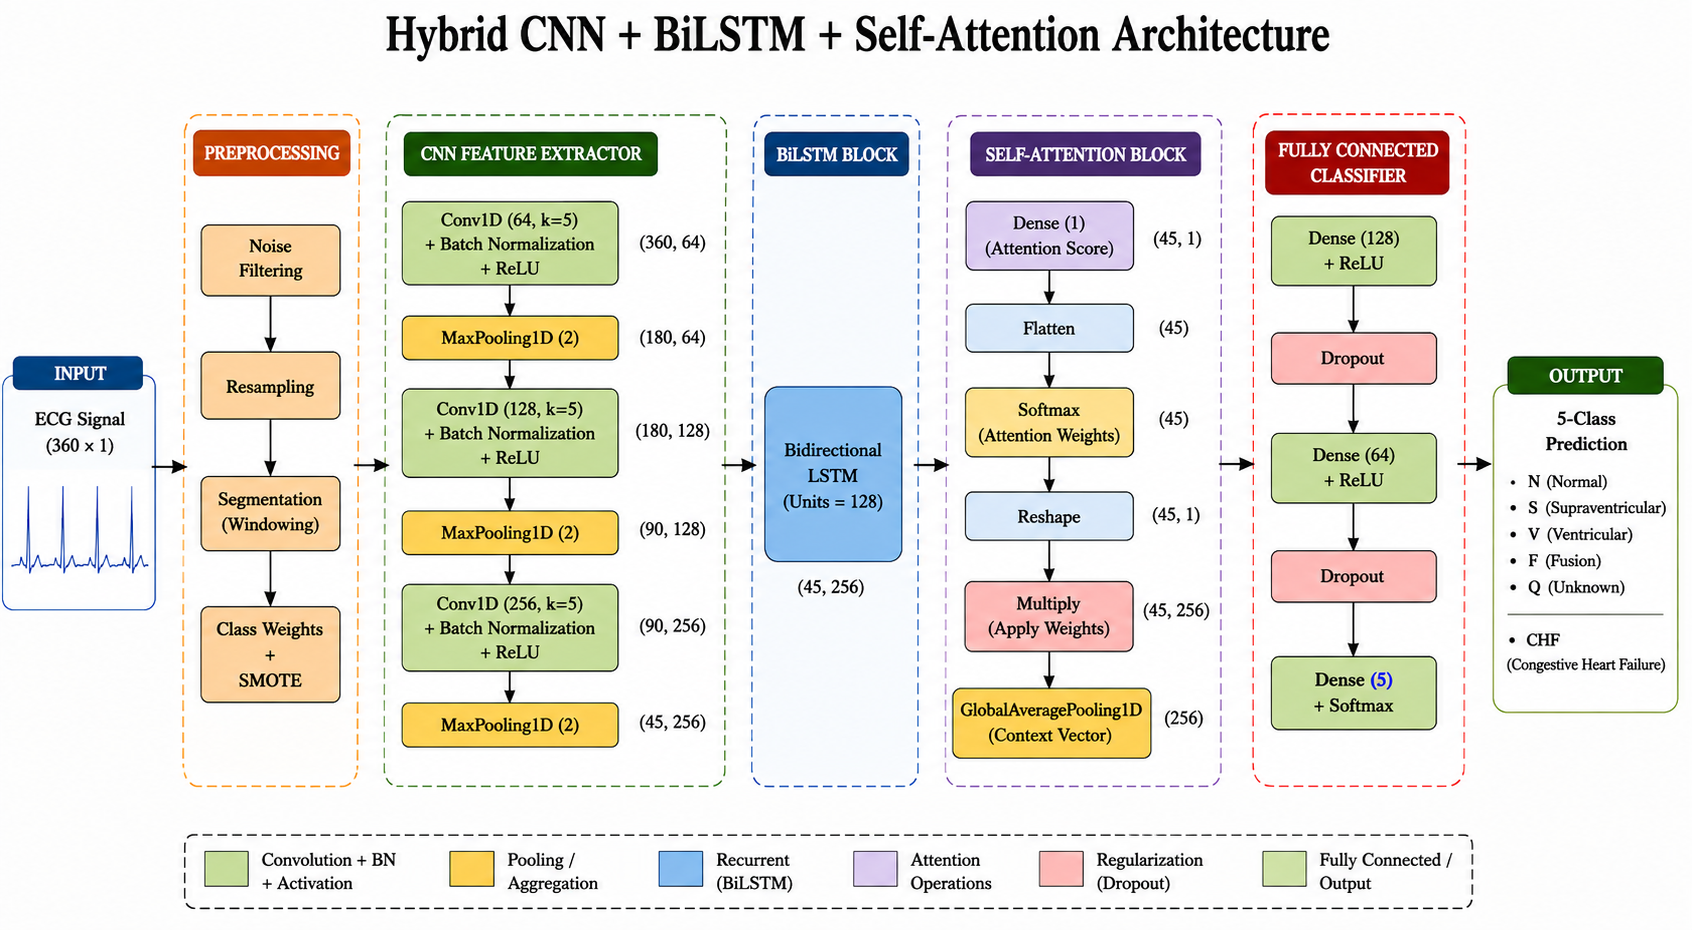
\includegraphics[width=0.95\linewidth]{figures/System_Architecture/hybrid_cnn_bilstm_attention.png}%
}{%
  \fbox{\parbox[c][2.6in][c]{0.92\linewidth}{\centering\footnotesize
    ADD THE HYBRID MODEL BLOCK DIAGRAM\\[4pt]
    \texttt{figures/System\_Architecture/}\\
    \texttt{hybrid\_cnn\_bilstm\_attention.png}}}%
}
\caption{Block diagram of the intra-patient CNN--BiLSTM--attention hybrid architecture}
\label{fig:hybrid_arch}
\end{figure}

\begin{equation}
  \alpha_{t} = \frac{\exp\left(\mathbf{v}^{\top}\tanh(\mathbf{W}\mathbf{h}_{t})\right)}{\sum_{t'}\exp\left(\mathbf{v}^{\top}\tanh(\mathbf{W}\mathbf{h}_{t'})\right)}
  \label{eq:attention}
\end{equation}

where $\mathbf{h}_{t}$ is the hidden state at time step $t$, and
$\mathbf{W}$ and $\mathbf{v}$ are learnable attention parameters. The
pooled waveform representation $\sum_{t}\alpha_{t}\mathbf{h}_{t}$ is
combined with a 48-unit dense branch that processes the auxiliary feature
vector, and the concatenation feeds the dense softmax classifier.

\subsection{MSFT-Net}

The comparison model, MSFT-Net, begins with three parallel
depthwise-separable convolutional blocks with kernel sizes 5, 11, and 21
samples followed by a single pointwise fusion layer. Three residual,
depthwise-separable stages follow, each including squeeze-and-excitation
(SE) channel gating and feature-wise linear modulation (FiLM) conditioned on
the auxiliary vector. SE gating reweights the channels of a feature map:

\begin{equation}
  \mathbf{x}' = \sigma\left(\mathbf{W}_{2}\,\mathrm{ReLU}(\mathbf{W}_{1}\,\mathrm{GAP}(\mathbf{x}))\right) \odot \mathbf{x}
  \label{eq:se}
\end{equation}

where GAP is global average pooling, $\sigma$ is the sigmoid function, and
$\odot$ is the Hadamard product. FiLM applies per-channel affine
conditioning derived from the auxiliary vector:

\begin{equation}
  \mathbf{y} = \boldsymbol{\gamma}(\mathbf{a}) \odot \mathbf{x} + \boldsymbol{\beta}(\mathbf{a})
  \label{eq:film}
\end{equation}

where $\boldsymbol{\gamma}$ and $\boldsymbol{\beta}$ are generated by dense
layers from the auxiliary vector $\mathbf{a}$. The overall data flow of
MSFT-Net -- the inter-patient deployment model -- is summarised in
Figure~\ref{fig:msft_arch}. The same late
auxiliary-feature fusion, global average pooling, and classification head
are used as in the hybrid. Two additional CNN-only and CNN--BiLSTM models
without attention were trained as ablation baselines, and the
microcontroller implementation used a separate single-input CNN.

% ----- Figure: inter-patient MSFT-Net architecture ------------------------
\begin{figure}[!t]
\centering
\IfFileExists{figures/System_Architecture/msft_net_architecture.png}{%
  % Portrait diagram (853x1280): sized below full text width to preserve
  % quality (>=200 dpi) and keep figure + caption on one page at natural ratio.
  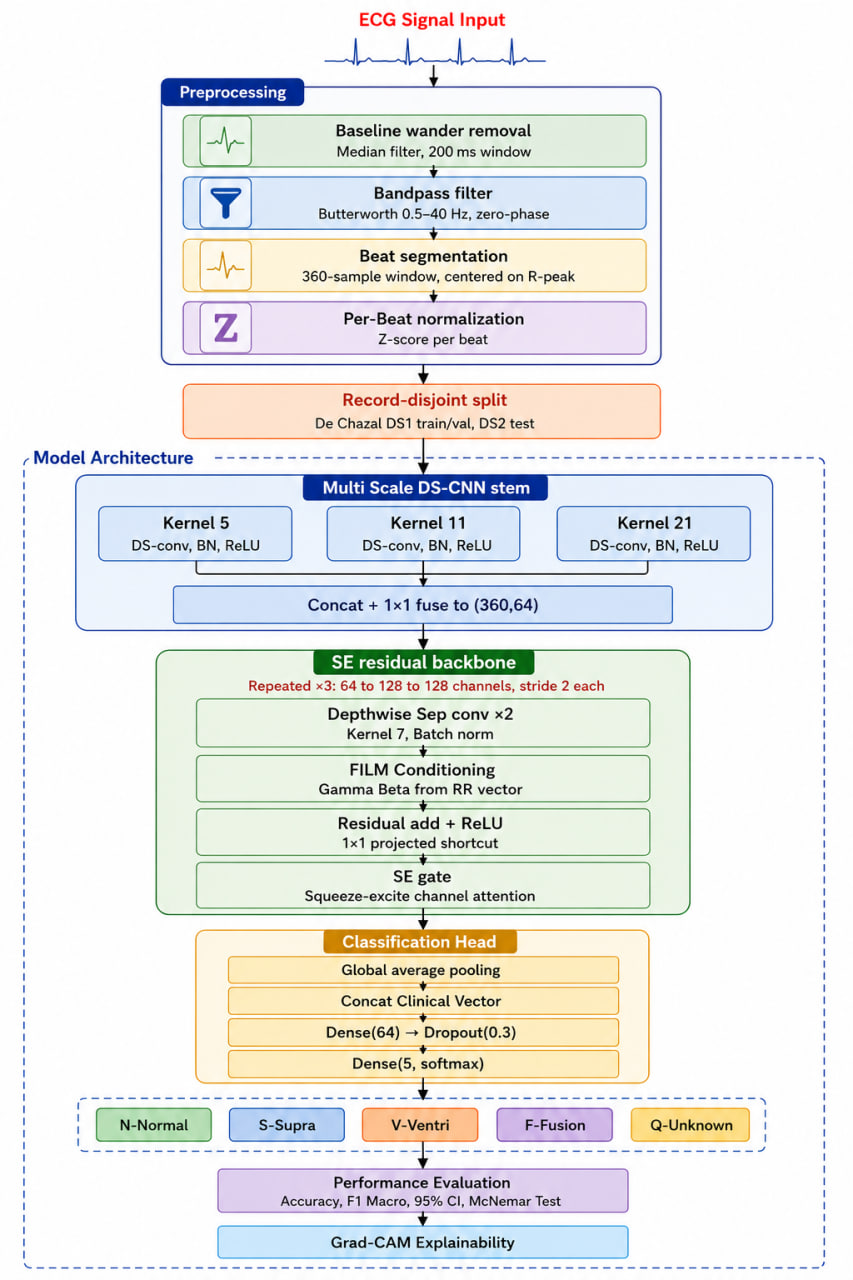
\includegraphics[width=0.95\linewidth]{figures/System_Architecture/msft_net_architecture.png}%
}{%
  \fbox{\parbox[c][2.6in][c]{0.92\linewidth}{\centering\footnotesize
    ADD THE MSFT-NET BLOCK DIAGRAM\\[4pt]
    \texttt{figures/System\_Architecture/}\\
    \texttt{msft\_net\_architecture.png}}}%
}
\caption{Block diagram of the inter-patient MSFT-Net architecture with multi-scale stem, squeeze-and-excitation, and FiLM conditioning}
\label{fig:msft_arch}
\end{figure}


\section{Proposed Methodology}
\label{sec:proposed_methodology}

\subsection{Sampling, labels, and record-disjoint partitioning}

The five AAMI groups were mapped to the MIT-BIH annotation symbols. Paced
records 102, 104, 107, and 217 were excluded from the N/S/V/F analysis;
because this rule filters out most $Q$ beats, beats from these records were
kept when the $Q$-class policy was enabled and excluded otherwise. Results
for $Q$ are therefore interpreted with caution, as they rest on very few
patients.

Records, rather than individual beats, were assigned to partitions to avoid
patient leakage, following the de~Chazal convention of separating the
records used for model development from those used for
testing \cite{dechazal2004}. A validation subset of the development records,
sharing no records with the test set, was reserved for early stopping.
Normal-sinus-rhythm and congestive-heart-failure records used in the
auxiliary analyses were likewise assigned by record identifier. Programmatic
checks ensured that no record appeared in more than one partition and that
all required classes were present in the training and test partitions.

Instead of enforcing a single global beat cap, beats were sampled with
per-record quotas via evenly spaced indices, so that every record
contributed observations and long recordings did not dominate the corpus.
Where possible, rare $S$ and $F$ beats were preserved. Splitting,
resampling, augmenting, scaling, template building, and imbalance correction
were applied only to the training partition.

\subsection{Fusion-beat treatment}

A staged intervention was designed for the fusion class: (i) global-average
pooling in place of attention pooling, (ii) $F$-specific augmentation,
(iii) $F/V$ hard-negative mining, and (iv) auxiliary $F$-vs-$N$ and
$F$-vs-$V$ heads. Each stage was studied in isolation in a dedicated
ablation arm so that its contribution could be measured rather than guessed
at.

\subsection{Microcontroller model}

A separate, single-input CNN was derived for the microcontroller
implementation. The model was quantised to full INT8 with
post-training quantisation using representative calibration beats, checked
against the TensorFlow Lite Micro operator set, and evaluated for accuracy
loss, latency, and memory footprint.


\section{System Workflow}
\label{sec:workflow}

\subsection{Training and imbalance handling}

Models were trained with the Adam optimiser, categorical cross-entropy
loss, a batch size of 64, and up to 50 epochs. Early stopping, learning-rate
decay on plateau, and checkpointing of the best model were all applied using
the validation set. Three class-imbalance strategies were compared: no
correction, a class-weighted loss function, and SMOTE oversampling applied
to the training data only, not the test data \cite{chawla2002smote}. Class
weights were calculated after oversampling and were never combined with
SMOTE. Auxiliary experiments applied conservative class-specific
augmentation, hard-negative mining (for $F$-vs-$V$ and $Q$), and auxiliary
heads (for $F$-vs-$N$, $F$-vs-$V$, and $Q$-vs-rest discrimination).


\section{Performance Evaluation Criteria}
\label{sec:eval_criteria}

\subsection{Primary metrics}

Class-specific sensitivity (Se) and positive predictivity ($+P$), reported
as both gross (pooled-beat) and average (per-record) figures, were the
primary results, as recommended by the ANSI/AAMI EC57 standard
\cite{aami_ec57_2012}. Precision--recall curves, precision at fixed recall,
macro-$F_1$, and accuracy were also reported. The macro-$F_1$ is defined as
the unweighted mean of the per-class $F_1$ scores, where each
$F_1 = 2 \cdot P \cdot R/(P + R)$ with $P$ the precision and $R$ the recall.

\subsection{Statistical analysis}

95\% confidence intervals for proportions were constructed using Wilson's
method \cite{wilson1927}. The 95\% confidence interval for macro-$F_1$ was
estimated with a nonparametric bootstrap using 2,000 resamples. Paired test
predictions were compared with the continuity-corrected McNemar test
\cite{mcnemar1947}, adjusted for multiple comparisons with the Holm
step-down procedure. All tests were two-tailed, and $P < 0.05$ was
considered statistically significant.

\subsection{Robustness and provenance}

Robustness was assessed under additive Gaussian noise (signal-to-noise
ratio from 20~dB down to 0~dB) and under increasing simulated baseline
wander. Source confounding was probed with a logistic-regression
discriminator trained to distinguish normal beats of the MIT-BIH database
from those of the normal-sinus-rhythm database, followed by a re-analysis
of the bandwidth-equalisation experiment.

\subsection{Explainability}

Model explanations were produced with Grad-CAM \cite{selvaraju2017gradcam},
attention weights, and Integrated Gradients \cite{sundararajan2017integrated}.
Faithfulness was assessed with deletion curves, which plot the decrease in
target-class probability after successively masking the most highly
attributed samples against the decrease from random masking.
% ==========================================================================
% CHAPTER 3 -- RESULTS AND DISCUSSION
%
% Presents what was obtained and explains what it means. All numbers are
% taken from the executed notebook outputs of the ASN manuscript study.
% ==========================================================================

\chapter{Results and Discussion}
\label{ch:results}

This chapter presents the results of the two evaluation protocols used in
this thesis and discusses their meaning. Section~\ref{sec:ch3_intro}
introduces the two protocols and their best-model results;
Section~\ref{sec:intra} reports the permissive intra-patient six-category
ECG study; Section~\ref{sec:inter} reports the record-disjoint inter-patient
five-class study, including the AAMI EC57 statistics, ablation analyses,
explainability, robustness, and microcontroller deployment;
Section~\ref{sec:crossprotocol} synthesises the two protocols; and
Section~\ref{sec:summary} closes with a summary of the findings.


\section{Introduction}
\label{sec:ch3_intro}

The proposed pipeline is evaluated under two deliberately different
protocols, and the contrast between them is itself one of the main themes of
this investigation. The first is an \emph{inter-patient}, record-disjoint
protocol based on the five ANSI/AAMI EC57 classes: normal (N),
supraventricular ectopic (S), ventricular ectopic (V), fusion (F), and
unknown/paced (Q)~\cite{aami_ec57_2012}, in which no patient contributes
beats to more than one partition. This is the regime under which arrhythmia
classifiers are comparable across studies, and it is much more difficult
because the model never sees a test patient during training. The second is
an \emph{intra-patient} protocol with a stratified train/validation/test
split and SMOTE balancing~\cite{chawla2002smote}, extended with a sixth
category comprising ECG segments derived from the BIDMC Congestive Heart
Failure Database (CHF). Because CHF is a cardiovascular clinical condition
rather than an ANSI/AAMI EC57 beat class, this arm is described throughout
as a six-\emph{category} ECG experiment rather than a six-class arrhythmia
problem; it is the more permissive, within-database regime frequently found
in the literature. The inter-patient protocol is the more stringent: it uses
a record-disjoint split so that no test patient's beats appear during
training, and it reports only the five AAMI EC57 classes. The intra-patient
protocol, by contrast, allows the same patient's beats in both training and
test partitions and adds a sixth, CHF-derived clinical-condition category.
The accuracy gap between the two arms---0.8945 versus 0.9859---quantifies
how much of the reported performance in the literature is an artefact of the
assessment regime rather than genuine generalisation.
Table~\ref{tab:protocols} compares the two protocols and their best-model
results. The intra-patient numbers cannot be compared with the inter-patient
numbers; the inter-patient protocol is the clinically meaningful one because
under a record-disjoint split none of the test patients' beats influenced
training.

\begin{table}[!t]
\centering
\caption{Comparison of the inter-patient (Part~A) and intra-patient (Part~B) evaluation protocols and their best-model results}
\label{tab:protocols}
\begin{tabular}{lcc}
\toprule
 & \textbf{Inter-patient (Part~A)} & \textbf{Intra-patient (Part~B)} \\
\midrule
Split                & record-disjoint          & stratified + SMOTE \\
Label set            & 5 AAMI classes (N/S/V/F/Q) & 5 + CHF-derived category \\
Balancing on test    & none                     & none \\
Test beats           & 9{,}112                  & 4{,}329 \\
Best accuracy        & 0.8945 (MSFT-Net)        & 0.9859 \\
Best macro-$F_1$     & 0.8725 (MSFT-Net)        & 0.9684 \\
\bottomrule
\end{tabular}
\end{table}

\section{Intra-Patient Six-Category Study}
\label{sec:intra}

The second protocol relaxes the record-disjoint constraint: a stratified
train/validation/test split is used, and a sixth category, comprising
R-peak-centred ECG segments derived from the BIDMC Congestive Heart Failure
Database, is added to the five AAMI beat categories to give a six-category
problem (N/S/V/F/Q plus a CHF-derived clinical-condition category)
evaluated on 4{,}329 test beats. This permissive, within-database regime is
widely used in the literature, and it is reported here both for completeness
and because its juxtaposition with the inter-patient results shows how much
apparent performance is a by-product of the assessment regime.

\subsection{Dataset Composition and Balancing}
\label{subsec:intra_data}

Beats were taken from the MIT-BIH Arrhythmia Database (48 records), the
MIT-BIH Normal Sinus Rhythm Database (18 records), which was mapped to the
normal class, and the BIDMC Congestive Heart Failure Database (15 records
at 250~Hz)~\cite{moody2001mitbih,goldberger2000physionet,baim1986chf}. The
normal and CHF contributions were each capped at 5{,}000 beats. Table
\ref{tab:intra_data} shows the composition from the raw extraction through
the normal-class cap to the SMOTE-balanced training set, and Figure
\ref{fig:intra_class_distribution} displays the raw imbalance.

\begin{table}[!t]
\centering
\caption[Composition of the intra-patient six-category ECG corpus]{Composition of the intra-patient six-category ECG corpus---five AAMI beat categories plus one CHF-derived clinical-condition category---from raw extraction through normal-class capping to the SMOTE-balanced training set}
\label{tab:intra_data}
\begin{tabular}{lrrr}
\toprule
\textbf{Class} & \textbf{Raw beats} & \textbf{After N-cap} & \textbf{Train (post-SMOTE)} \\
\midrule
N-Normal  & 10{,}000 & 5{,}000 & 5{,}627 \\
S-Supra   &  2{,}781 & 2{,}781 & 5{,}627 \\
V-Ventri  &  7{,}235 & 7{,}235 & 5{,}627 \\
F-Fusion  &    802  &    802  & 5{,}627 \\
Q-Unknown &  8{,}038 & 8{,}038 & 5{,}627 \\
CHF       &  5{,}000 & 5{,}000 & 5{,}627 \\
\midrule
Total     & 33{,}856 & 28{,}856 & 33{,}762 \\
\bottomrule
\end{tabular}
\end{table}

\begin{figure}[!t]
\centering
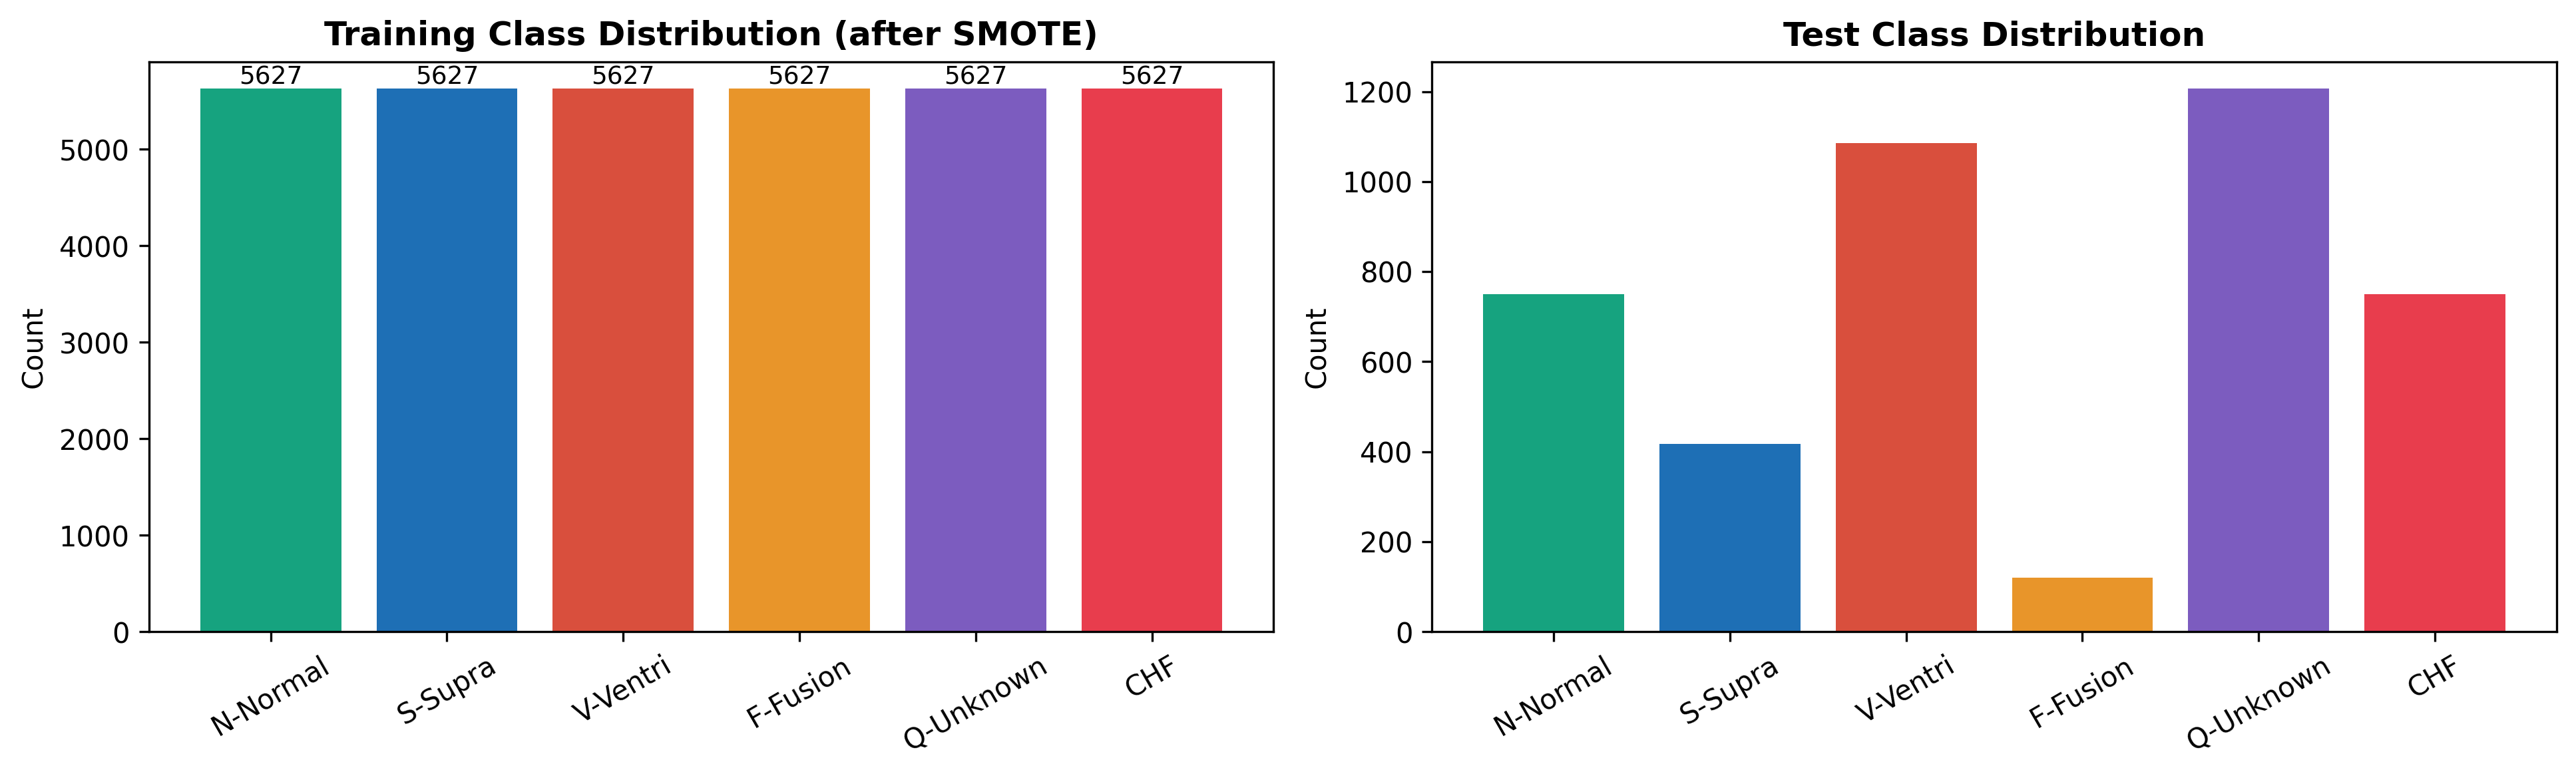
\includegraphics[width=0.95\linewidth]{figures/Intra_Patient/00_class_distribution.png}
\caption{Raw class distribution of the six-category intra-patient corpus before balancing}
\label{fig:intra_class_distribution}
\end{figure}

The data in Table~\ref{tab:intra_data} make two design decisions explicit.
Capping the normal class prevents the majority class from dominating the
SMOTE targets, and equalising the six training categories to 5{,}627 beats
avoids class imbalance as a confounding factor during optimisation. Both
choices are sensible for maximising within-database accuracy, but neither
concerns generalisation between patients, precisely because the split is
not record-disjoint, which is why the numbers below are substantially
higher than those of the inter-patient part.

\subsection{Training Dynamics and Overall Accuracy}
\label{subsec:intra_perf}

The CNN--BiLSTM--Attention model was trained for up to 50 epochs with early
stopping; Figure~\ref{fig:intra_training} shows how the learning curves
evolve. The overall test accuracy of the full model is 0.9859, with a
macro-$F_1$ of 0.9684. As Table~\ref{tab:intra_perclass} shows, five of the
six categories achieve $F_1$ scores of 0.96 or better; only the fusion class
remains difficult, with an $F_1$ of 0.84.

\begin{figure}[!t]
\centering
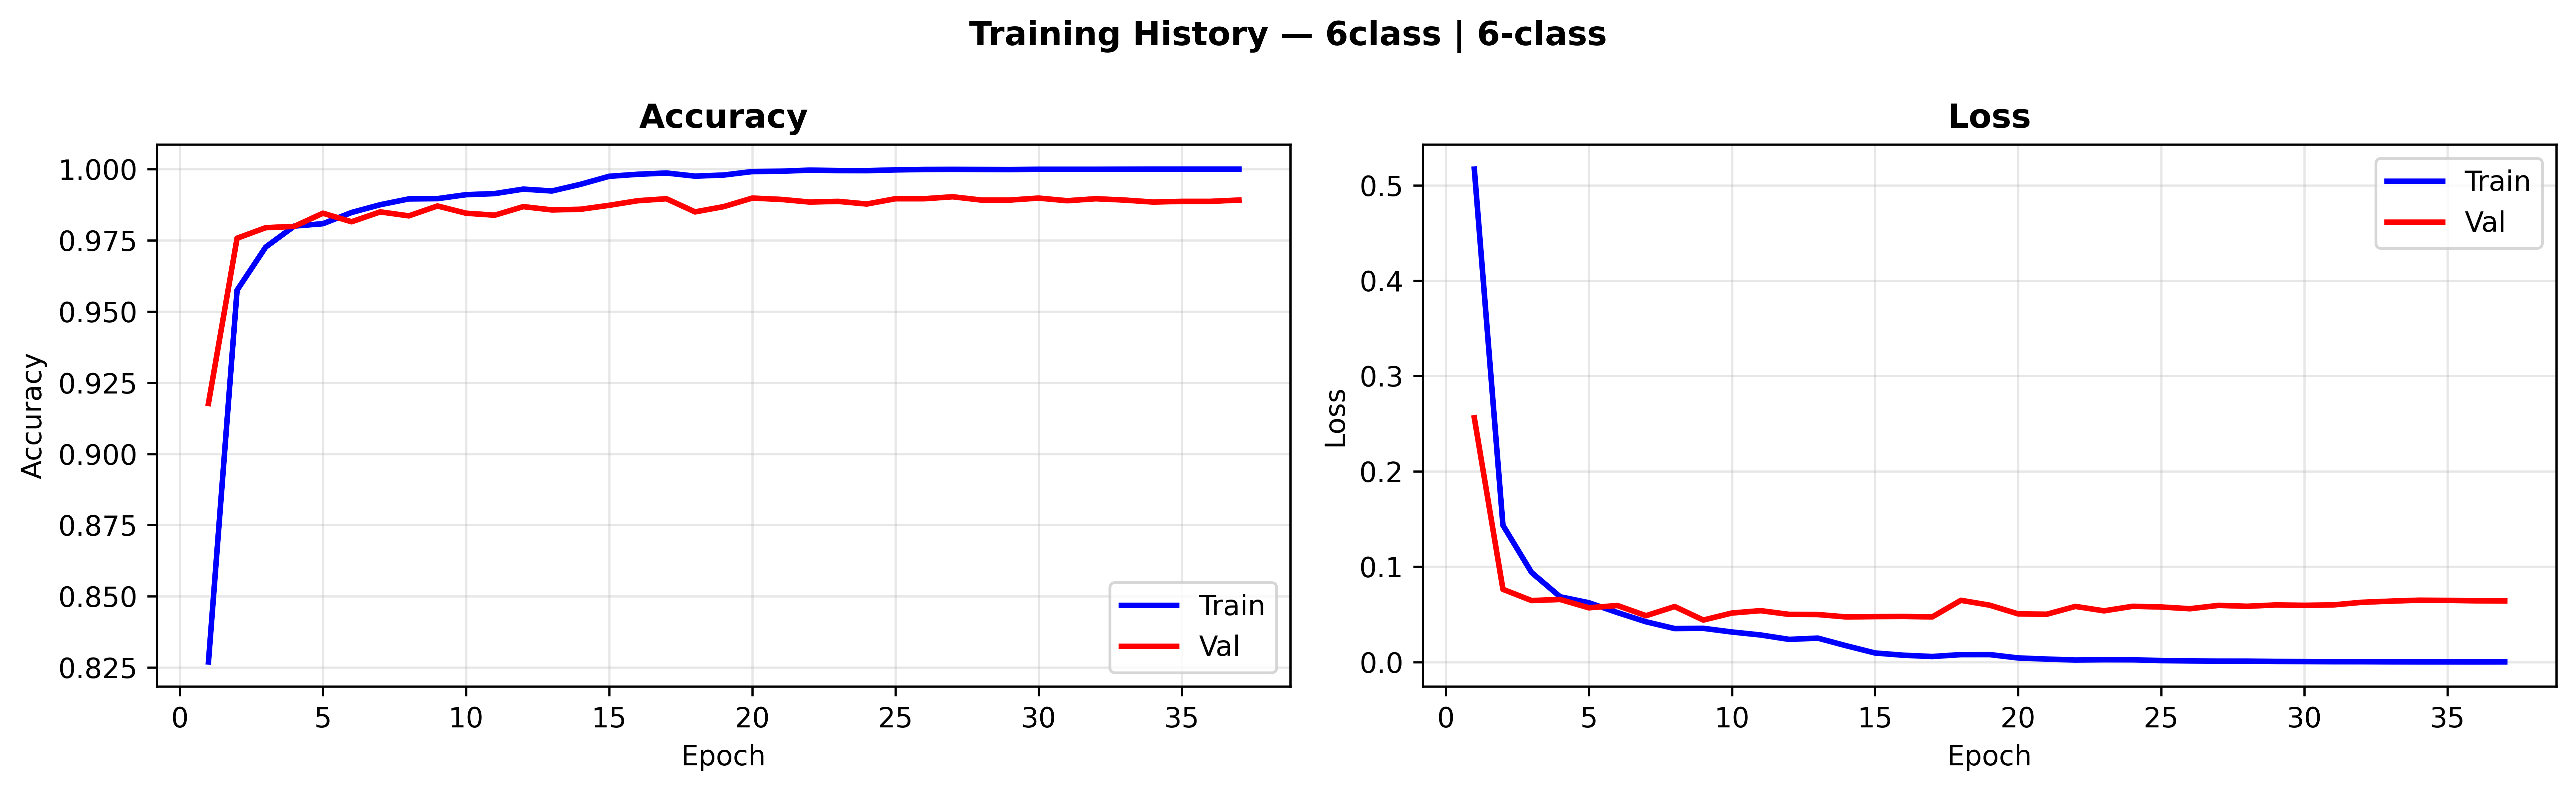
\includegraphics[width=0.95\linewidth]{figures/Intra_Patient/04_training_history.png}
\caption{Training and validation curves for the six-category hybrid under the intra-patient protocol}
\label{fig:intra_training}
\end{figure}

\begin{table}[!t]
\centering
\caption[Per-class precision, recall, and $F_1$ on the intra-patient six-category test set]{Per-class precision, recall, and $F_1$ on the intra-patient six-category test set (representative single-run report); CHF denotes the CHF-derived clinical-condition category}
\label{tab:intra_perclass}
\begin{tabular}{lrrrr}
\toprule
\textbf{Class} & \textbf{Precision} & \textbf{Recall} & \textbf{$F_1$} & \textbf{Support} \\
\midrule
N-Normal  & 0.99 & 1.00 & 0.99 & 750 \\
S-Supra   & 0.95 & 0.97 & 0.96 & 417 \\
V-Ventri  & 0.98 & 0.97 & 0.97 & 1{,}086 \\
F-Fusion  & 0.83 & 0.86 & 0.84 & 120 \\
Q-Unknown & 1.00 & 0.99 & 0.99 & 1{,}206 \\
CHF       & 1.00 & 0.99 & 0.99 & 750 \\
\midrule
Macro avg & 0.96 & 0.96 & 0.96 & 4{,}329 \\
Accuracy  & \multicolumn{3}{c}{0.9859} & 4{,}329 \\
\bottomrule
\end{tabular}
\end{table}

The CHF result must be interpreted with caution. As discussed in
Section~\ref{subsec:provenance}, the CHF segments come from a different
database with a different sampling frequency than the arrhythmia records, so
a large fraction of the model's CHF separability is likely due to a database
``fingerprint'' rather than cardiac morphology; it should not be read as
evidence of a clinically generalisable CHF signature. It is for this reason
that CHF was excluded from the rigorous five-class study. The one class that
remains difficult even under the permissive protocol is fusion: its $F_1$ of
0.84 even when training and test patients coincide is evidence that the
fusion difficulty is genuinely morphological, not an artefact of the
record-disjoint split, and it retrospectively validates the dedicated
fusion-handling pipeline of Section~\ref{subsec:fbeat}.

\subsection{Confusion Structure and ROC}
\label{subsec:intra_cm}

Figures~\ref{fig:intra_cm} and~\ref{fig:intra_roc} present the six-category
confusion matrix and the one-versus-rest ROC curves. The residual error is
concentrated in the fusion row and column, mirroring the inter-patient
finding that fusion is the binding constraint on performance. The ROC curves
are practically saturated, which is the logical result of a subject-mixed
split: at test time the model has already seen the typical waveform of each
patient, so detecting that patient's beat types is a much simpler problem
than picking out beat types on a patient it has never seen. This is the
quantitative centre of the cross-protocol comparison in
Section~\ref{sec:crossprotocol}.

\begin{figure}[!t]
\centering
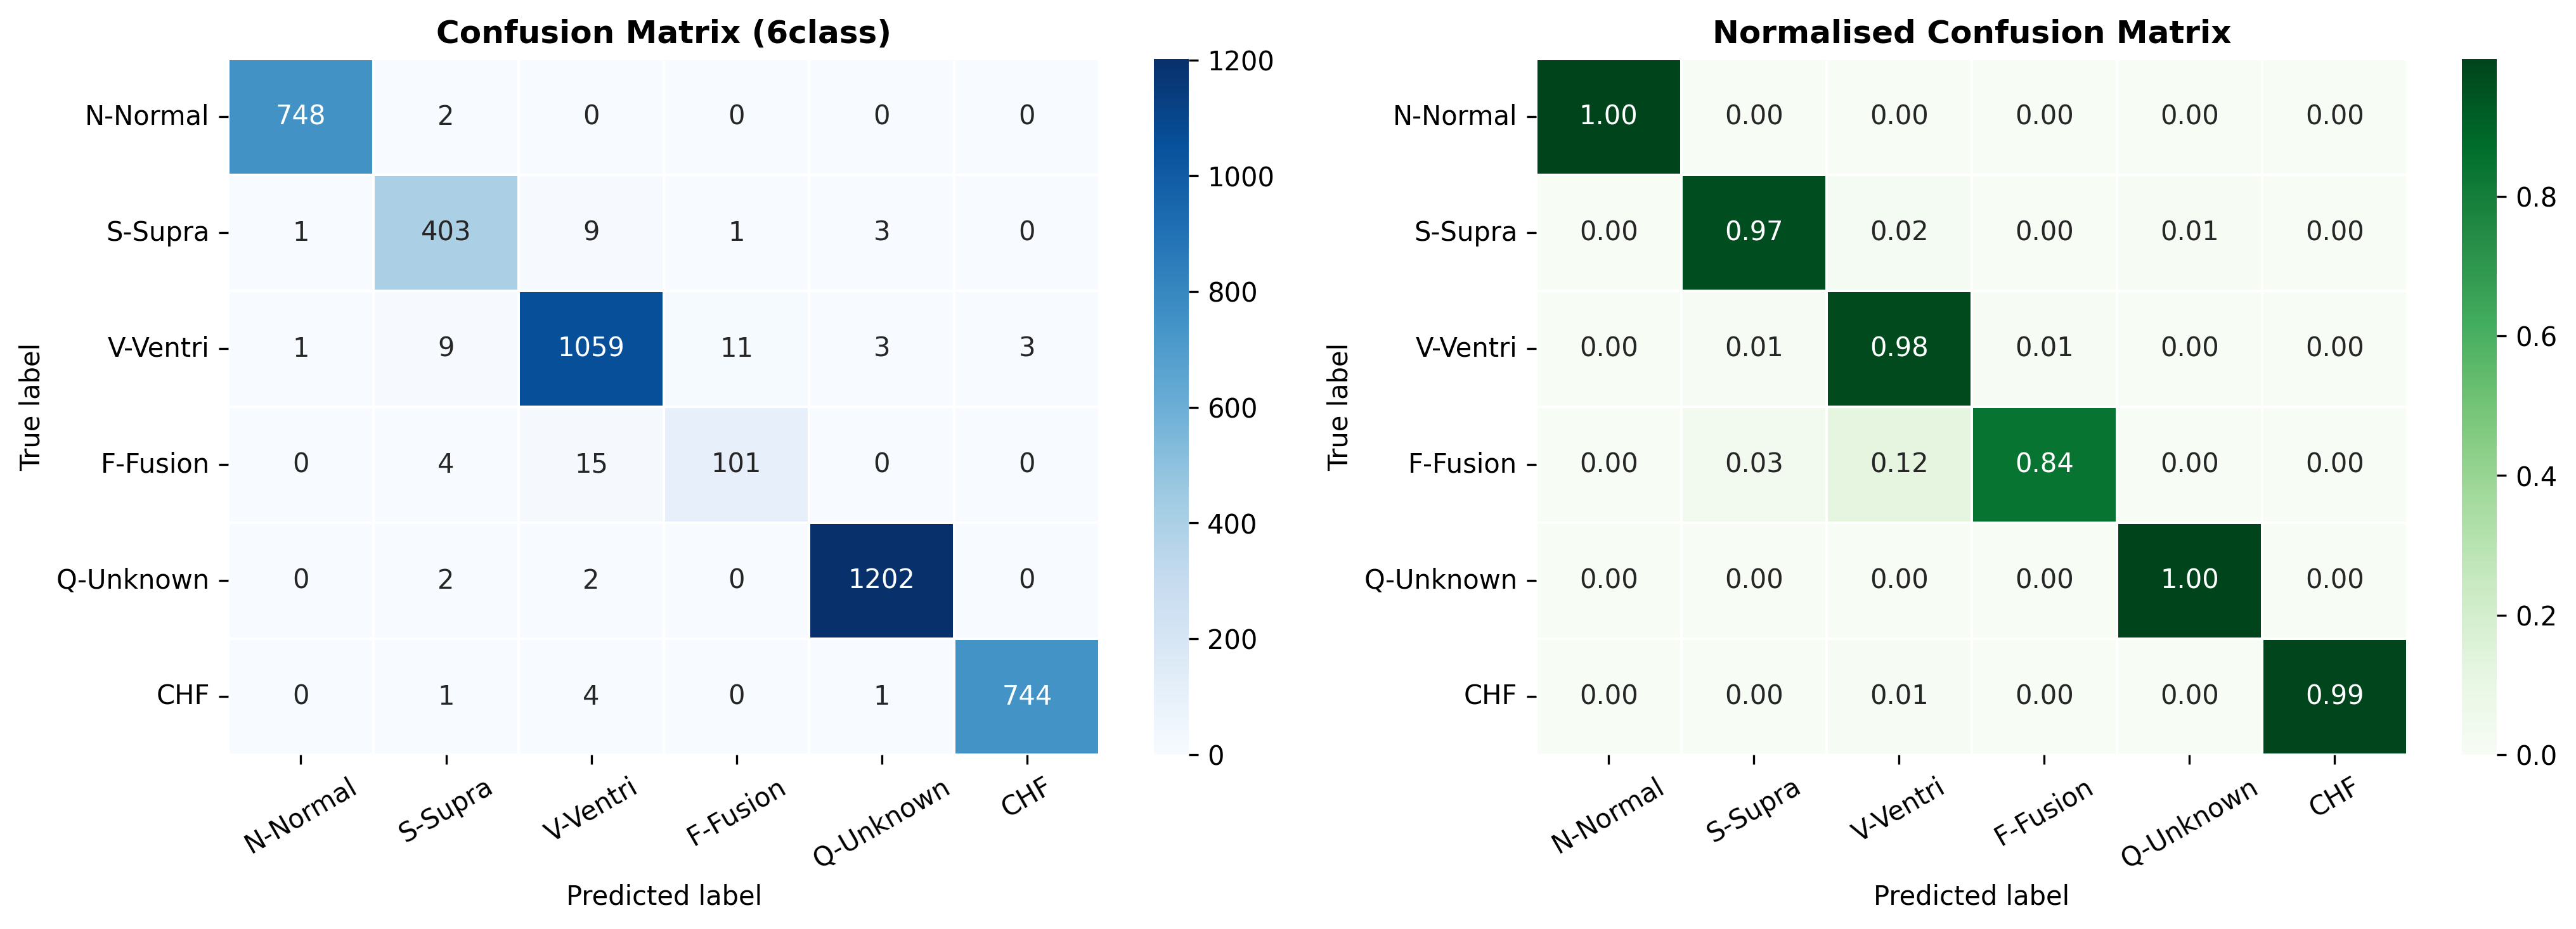
\includegraphics[width=0.95\linewidth]{figures/Intra_Patient/02_confusion_matrix.png}
\caption{Confusion matrix for the six-category intra-patient ECG classification experiment}
\label{fig:intra_cm}
\end{figure}

\begin{figure}[!t]
\centering
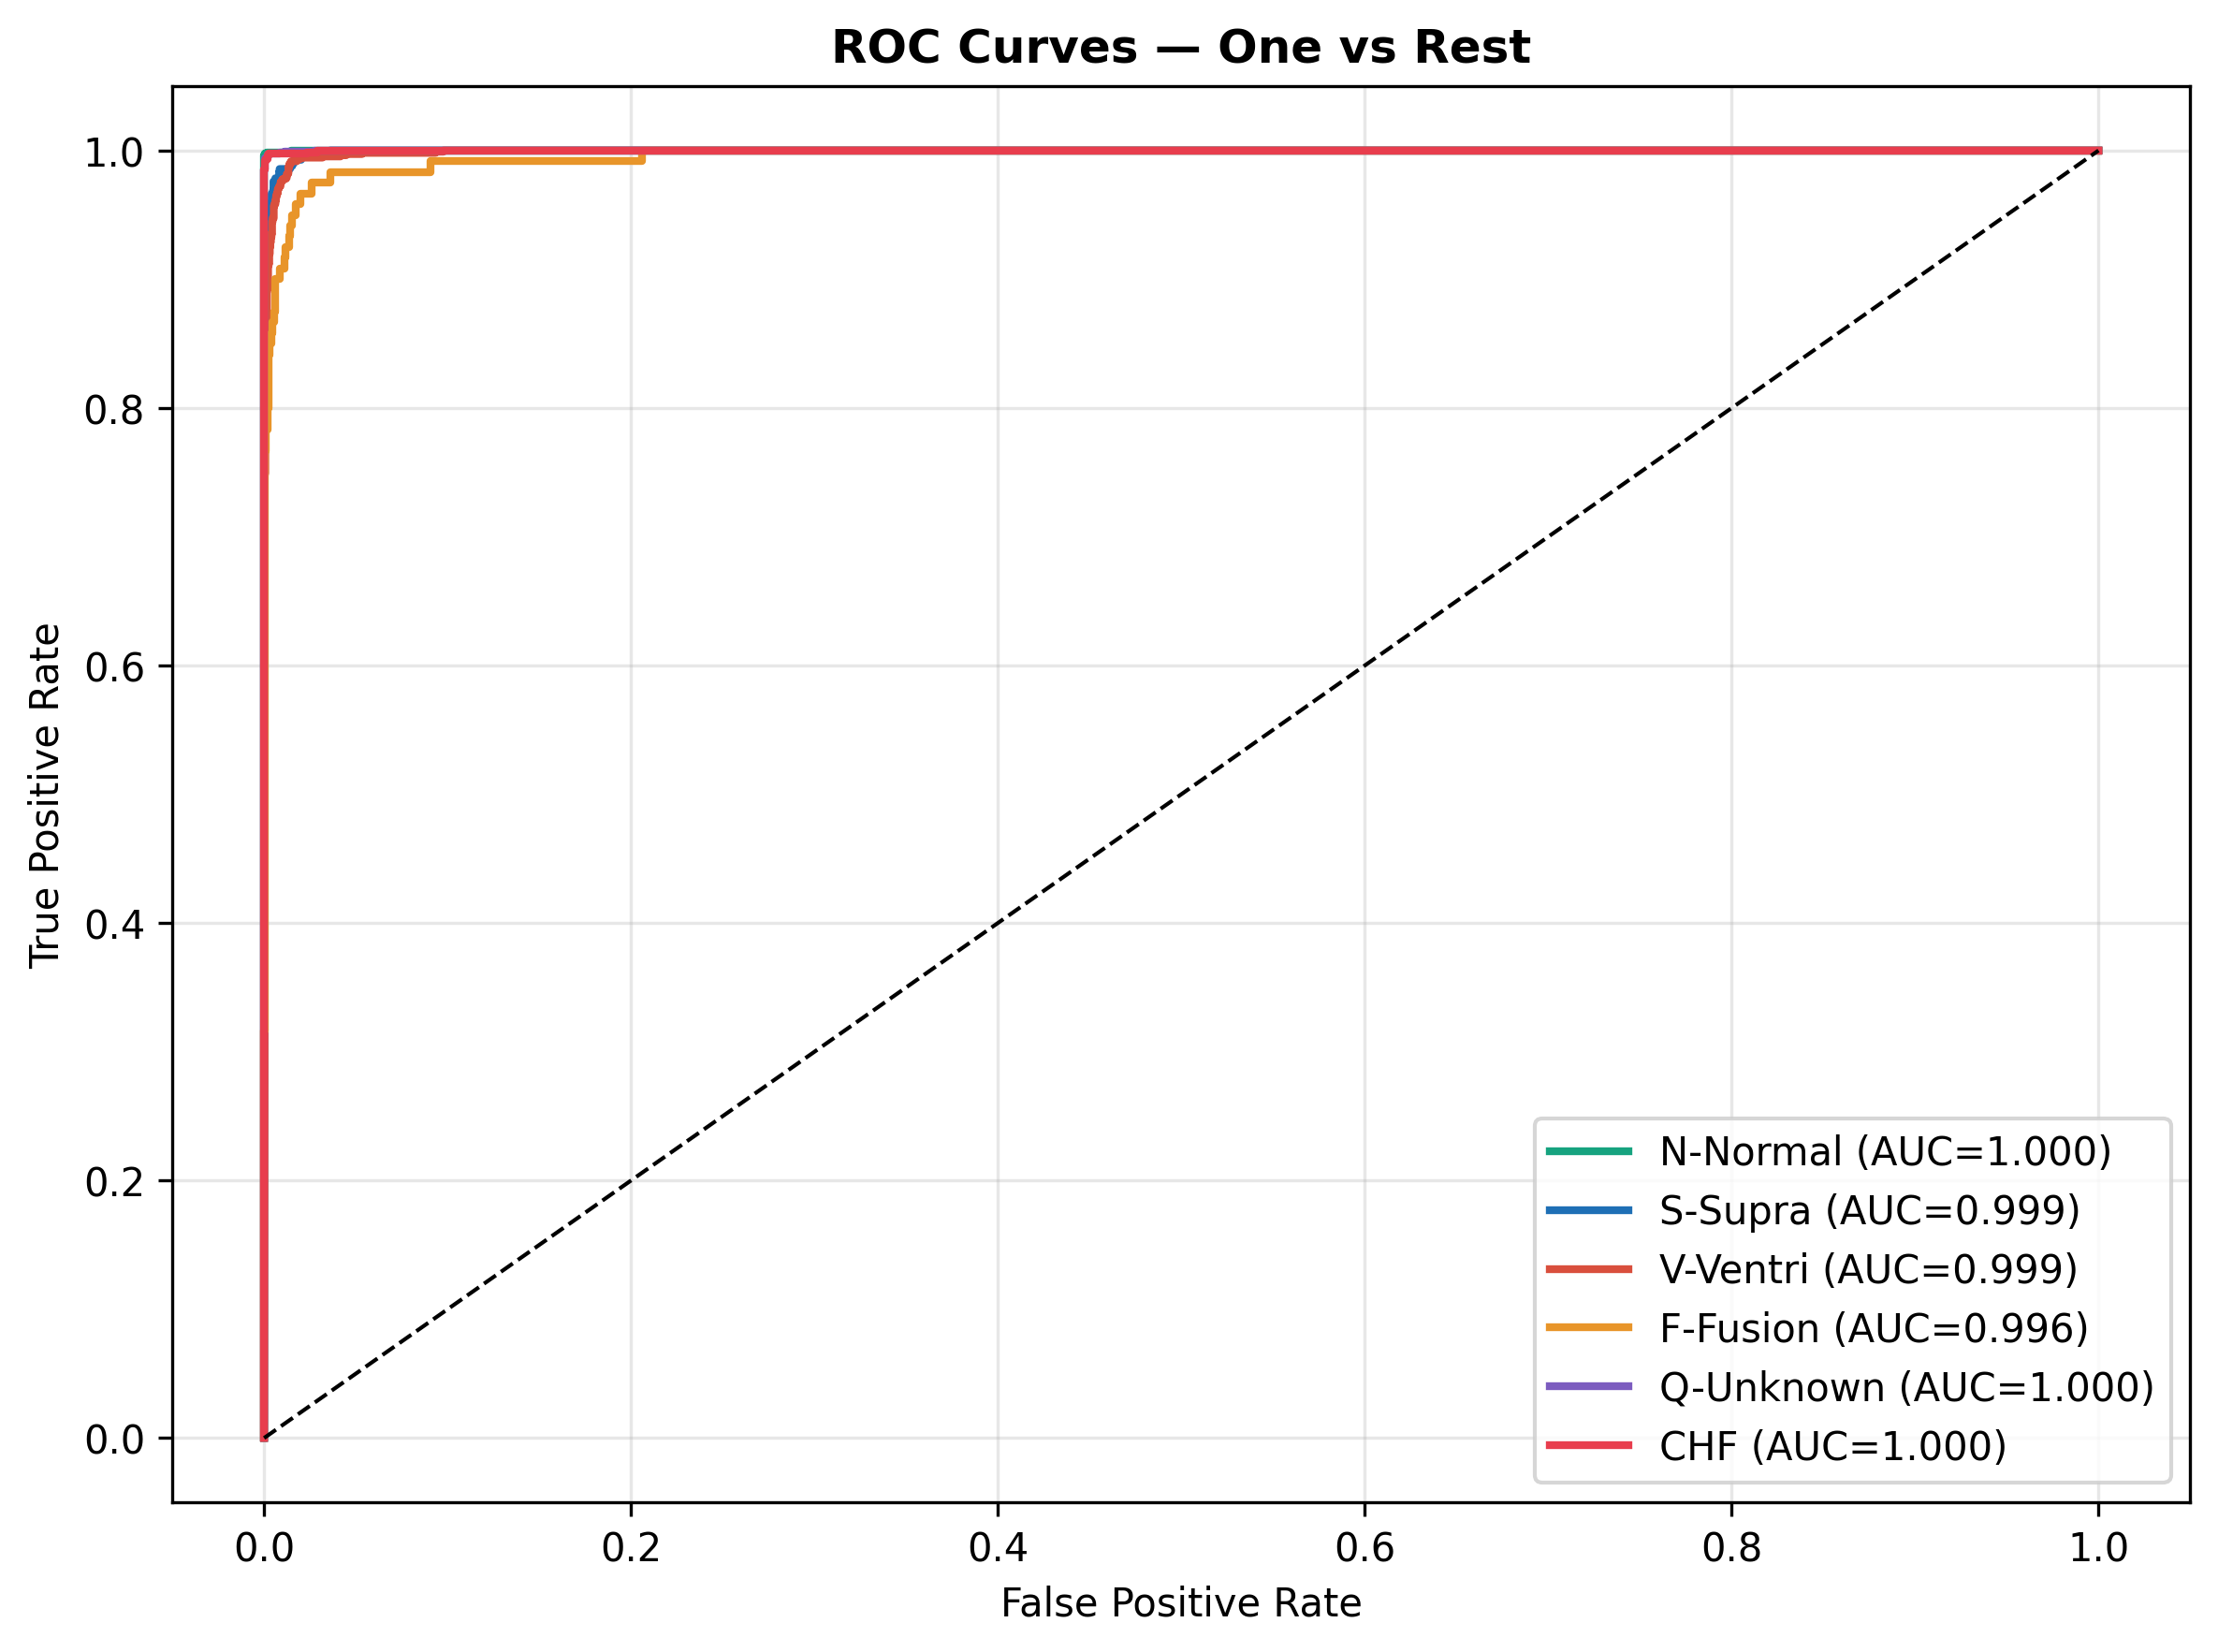
\includegraphics[width=0.75\linewidth]{figures/Intra_Patient/03_roc_curves.png}
\caption{One-versus-rest ROC curves for the six-category intra-patient ECG classification experiment}
\label{fig:intra_roc}
\end{figure}

\subsection{Ablation: Contribution of the Recurrent and Attention Stages}
\label{subsec:intra_ablation}

Table~\ref{tab:intra_ablation} and Figure~\ref{fig:intra_ablation} isolate
the contribution of the BiLSTM and attention stages by progressively
building the architecture from a CNN-only baseline.

\begin{table}[!t]
\centering
\caption{Architecture ablation under the intra-patient protocol}
\label{tab:intra_ablation}
\begin{tabular}{lrrr}
\toprule
\textbf{Model} & \textbf{Accuracy} & \textbf{Macro-$F_1$} & \textbf{$\Delta$Acc} \\
\midrule
CNN only                            & 0.9799 & 0.9604 & -- \\
CNN + BiLSTM                        & 0.9843 & 0.9660 & $+0.0044$ \\
CNN + BiLSTM + Attention (proposed) & 0.9834 & 0.9649 & $+0.0035$ \\
\bottomrule
\end{tabular}
\end{table}

\begin{figure}[!t]
\centering
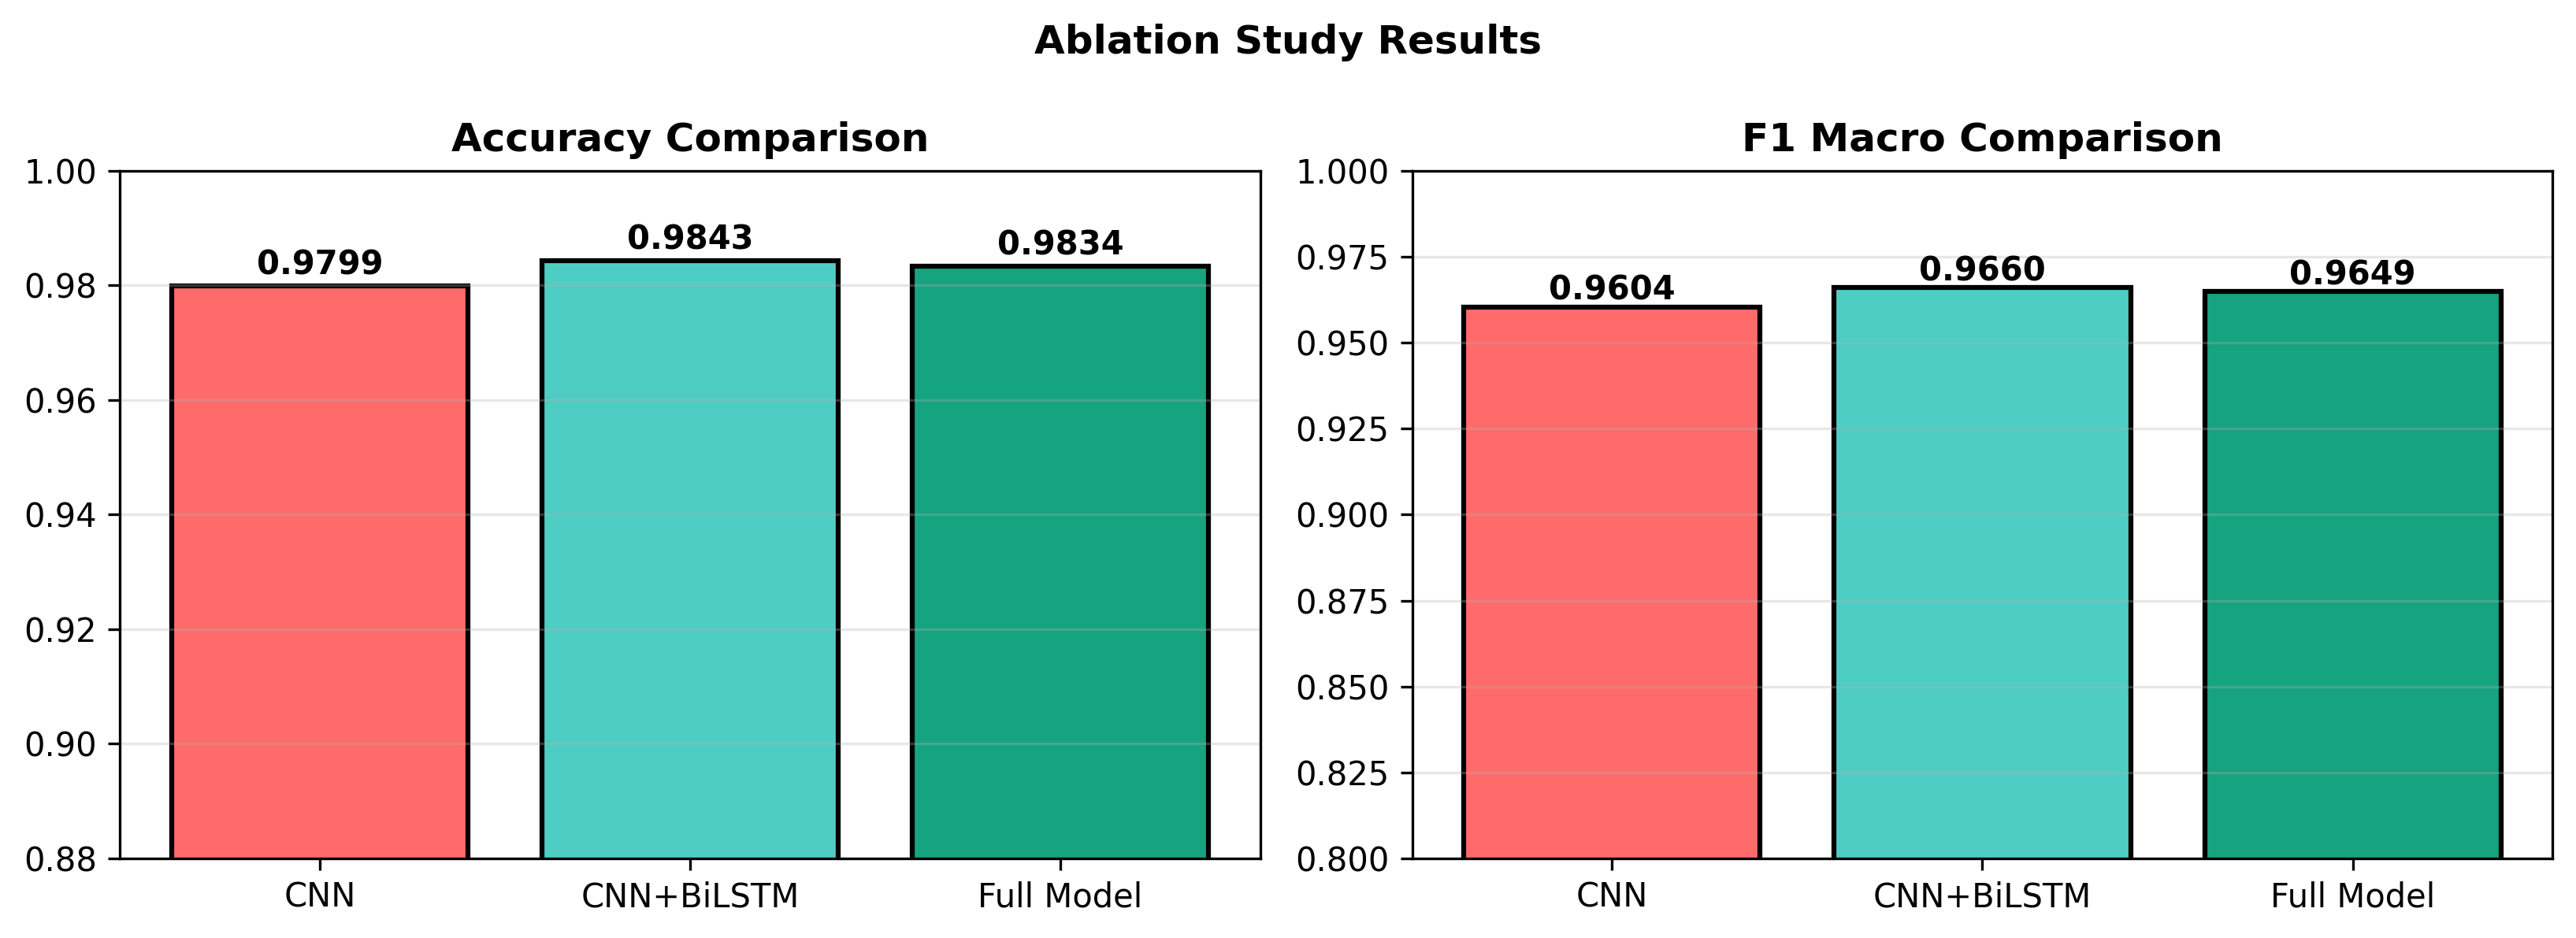
\includegraphics[width=0.95\linewidth]{figures/Intra_Patient/05_ablation.png}
\caption{Accuracy and macro-$F_1$ across the three architecture arms under the intra-patient protocol}
\label{fig:intra_ablation}
\end{figure}

Table~\ref{tab:intra_ablation} contains an instructive result that directly
contradicts what will be found under the record-disjoint split: the BiLSTM
stage contributes a measurable accuracy gain of 0.0044 (and a macro-$F_1$
gain of 0.0056) under the subject-mixed
split, while the attention stage adds nothing further (accuracy in fact
decreases by 0.0009). The recurrent stage exploits patient-dependent temporal regularities
that are present in a subject-mixed split but absent, by design, from the
held-out patients of a record-disjoint split. In other words, part of what
the recurrent stage learns is not transferable arrhythmia morphology but
patient identity. This is a concrete, data-based demonstration of why the
evaluation protocol changes not only the numbers reported but also the
architectural conclusions drawn from them.

\subsection{Model Compression}
\label{subsec:intra_compress}

The six-category hybrid was also compressed for edge deployment. Dynamic-range
quantisation reduced the converted lightweight model from 1.21~MB to
0.14~MB, an 88.42\% reduction, but the measured test accuracy dropped to
0.1737, just above the 0.167 chance level for the six-way problem. The dynamic-range
conversion, applied without a representative calibration data set, did not
maintain the decision function. This is reported as an intentional negative
result: it contrasts with the inter-patient INT8 model of
Section~\ref{subsec:mcu}, which was quantised with proper post-training
integer calibration. The practical lesson is that aggressive compression is
feasible only when faithful low-bit quantisation is performed with
appropriate calibration data, not by dynamic-range conversion alone.

\subsection{Comparison with Reported Methods}
\label{subsec:intra_sota}

Table~\ref{tab:sota} restates the comparison found in the executed
notebook, comparing the intra-patient six-category model against representative
reported ECG-classification methods. Because the studies are based on
different databases, class groupings, and, most importantly, different
train/test protocols, the comparison is indicative only; the numbers are
not to be read as a like-for-like ranking.

\begin{table}[!t]
\centering
\caption{Indicative comparison of the intra-patient six-category model with reported ECG-classification methods}
\label{tab:sota}
\setlength{\tabcolsep}{3.5pt}%
\begin{tabular}{@{}>{\raggedright\arraybackslash}p{1.7in}>{\raggedright\arraybackslash}p{1.7in}ccc@{}}
\toprule
\textbf{Method} & \textbf{Dataset} & \textbf{Categories} & \textbf{Accuracy} & \textbf{Macro-$F_1$} \\
\midrule
This work\newline(CNN+BiLSTM+Att.\ +XAI) & MIT-BIH+NSR+CHF & 6 & 0.9859 & 0.9684 \\
CNN--BiLSTM+Att                 & MIT-BIH         & 5 & 0.9920 & 0.9750 \\
CNN+LSTM+Att                    & MIT-BIH+PTB     & 5 & 0.9930 & 0.9600 \\
Transformer ECG                 & MIT-BIH         & 5 & 0.9832 & 0.9501 \\
DenseNet1D                      & MIT-BIH         & 5 & 0.9756 & 0.9234 \\
LSTM--FCN                       & MIT-BIH         & 5 & 0.9634 & 0.8967 \\
SVM baseline                    & MIT-BIH         & 5 & 0.8976 & 0.7832 \\
\bottomrule
\end{tabular}
\end{table}

Table~\ref{tab:sota} puts the intra-patient model in perspective: it
achieves roughly the same performance as recent deep learning approaches,
with two characteristics that most of them lack: a six-category label set
that adds a CHF-derived category, and multi-database training. The most honest
interpretation of this table, however, is comparative rather than
competitive: several listed methods report slightly higher accuracy on the
narrower five-class MIT-BIH problem, and none of the external numbers was
obtained under a record-disjoint protocol. The results of
Section~\ref{sec:inter} show that Part~A is the more challenging and
clinically important test, so the meaning of the present work is not to sit
at the head of this table but to report both protocols transparently so
that apparent performance differences can be attributed to their real
source.


\section{Inter-Patient (Record-Disjoint) Five-Class Study}
\label{sec:inter}

All metrics in this section are calculated on a frozen inter-patient test
partition of 9{,}112 beats from 26 patients of the MIT-BIH Arrhythmia
Database~\cite{moody2001mitbih,goldberger2000physionet}.

\subsection{Dataset Composition and Partitioning}
\label{subsec:dataset}

The beat corpus was assembled from three source types: 48 MIT-BIH records
covering multiple rhythms, 18 MIT-BIH Normal Sinus Rhythm records used to
augment the normal class, and a congestive-heart-failure set that was not
included in the final label space following the provenance controls of
Section~\ref{subsec:provenance}. To keep the study EC57-conformant, the four
paced records (102, 104, 107, 217) contribute $Q$ beats only, so that the
N/S/V/F supports are equivalent to a paced-free run. Table~\ref{tab:dataset}
summarises the class-wise beat counts, the record-disjoint split, and the
record coverage; the resulting class imbalance is visualised in
Figure~\ref{fig:class_distribution}. Two consequences of the sampling rules
deserve emphasis. First, because the per-record quotas of
Section~\ref{sec:proposed_methodology} preserve every available $S$ and $F$
beat, the $S$ and $F$ totals equal their complete raw populations (2,781 and
802 beats, identical to the raw extraction of Section~\ref{subsec:intra_data}),
whereas the abundant $N$, $V$, and $Q$ classes are bounded by the quotas.
The comparatively small $V$ total (667 beats) therefore reflects quota
sampling rather than the underlying prevalence of ventricular ectopy, and
the per-class test supports should be read in this light.

\begin{table}[!t]
\centering
\caption{Beat-level composition of the five AAMI classes and the record-disjoint partitioning}
\label{tab:dataset}
\begin{tabular}{lrrrrr}
\toprule
\textbf{Class} & \textbf{Records} & \textbf{Total beats} & \textbf{Train} & \textbf{Val.} & \textbf{Test} \\
\midrule
N-Normal   & 58 & 15{,}306 & 7{,}455 & 1{,}804 & 6{,}047 \\
S-Supra    & 32 &  2{,}781 &   774   &   170   & 1{,}837 \\
V-Ventri   & 25 &    667   &   283   &    51   &   333   \\
F-Fusion   & 17 &    802   &   399   &    15   &   388   \\
Q-Unknown  &  9 &  2{,}015 & 1{,}008 &   500   &   507   \\
\midrule
Total      & -- & 21{,}571 & 9{,}919 & 2{,}540 & 9{,}112 \\
\bottomrule
\end{tabular}
\end{table}

\begin{figure}[!t]
\centering
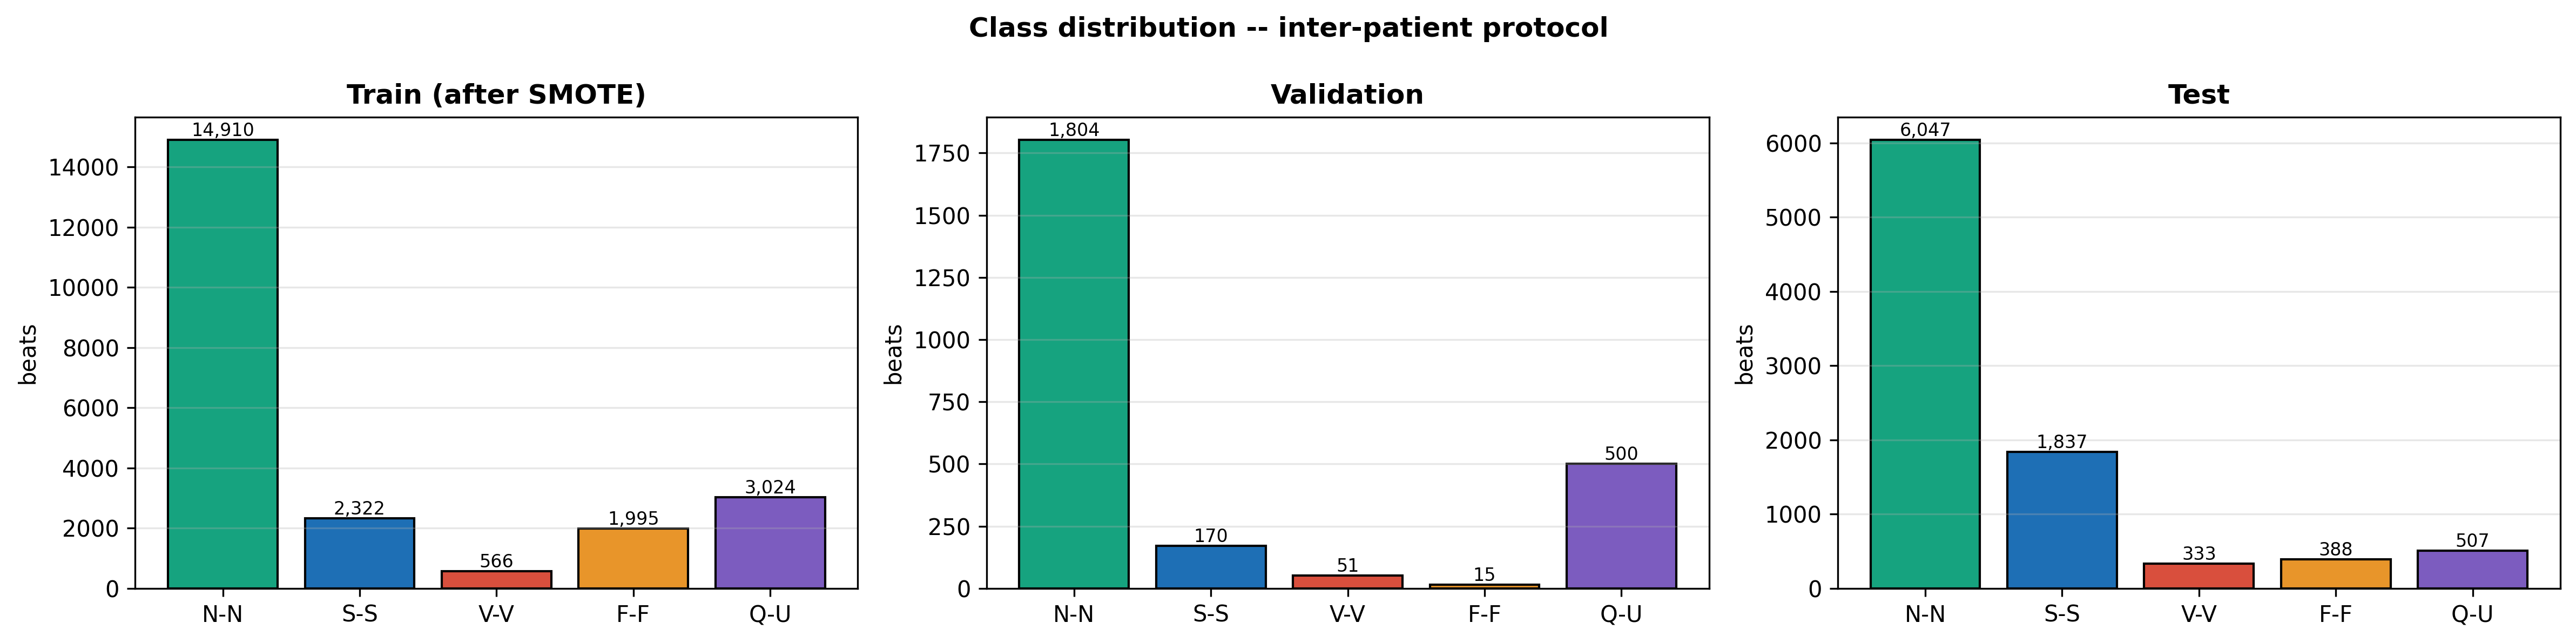
\includegraphics[width=0.95\linewidth]{figures/Inter_Patient/00_class_distribution.png}
\caption{Class distribution of the assembled beat corpus under the inter-patient protocol}
\label{fig:class_distribution}
\end{figure}

The class distribution in Figure~\ref{fig:class_distribution} is strongly
imbalanced and clinically representative: fusion and ventricular beats
occur rarely, yet they are the most expensive to miss when diagnosing.
Training-only augmentation was applied to the minority classes (one
perturbed copy of every training $S$ beat and three additional copies of
every training $F$ beat), adding 1{,}971 beats and expanding the training
set from 9{,}919 to 11{,}890
beats, while validation and test partitions were left untouched. The RR
timing, QRS morphology, wavelet descriptors, and N/V-template-similarity
features were computed from training statistics only, without using
validation or test labels, so the scale of any feature or template cannot
be contaminated by test information.

\subsection{Training Dynamics}
\label{subsec:training}

Figures~\ref{fig:train_hybrid} and~\ref{fig:train_msft} show the learning
curves of the two architectures: the CNN--BiLSTM--Attention hybrid (572{,}358
parameters) and the lighter MSFT-Net (167{,}090 parameters) with multi-scale
convolutions, squeeze-and-excitation, and FiLM conditioning.

\begin{figure}[!t]
\centering
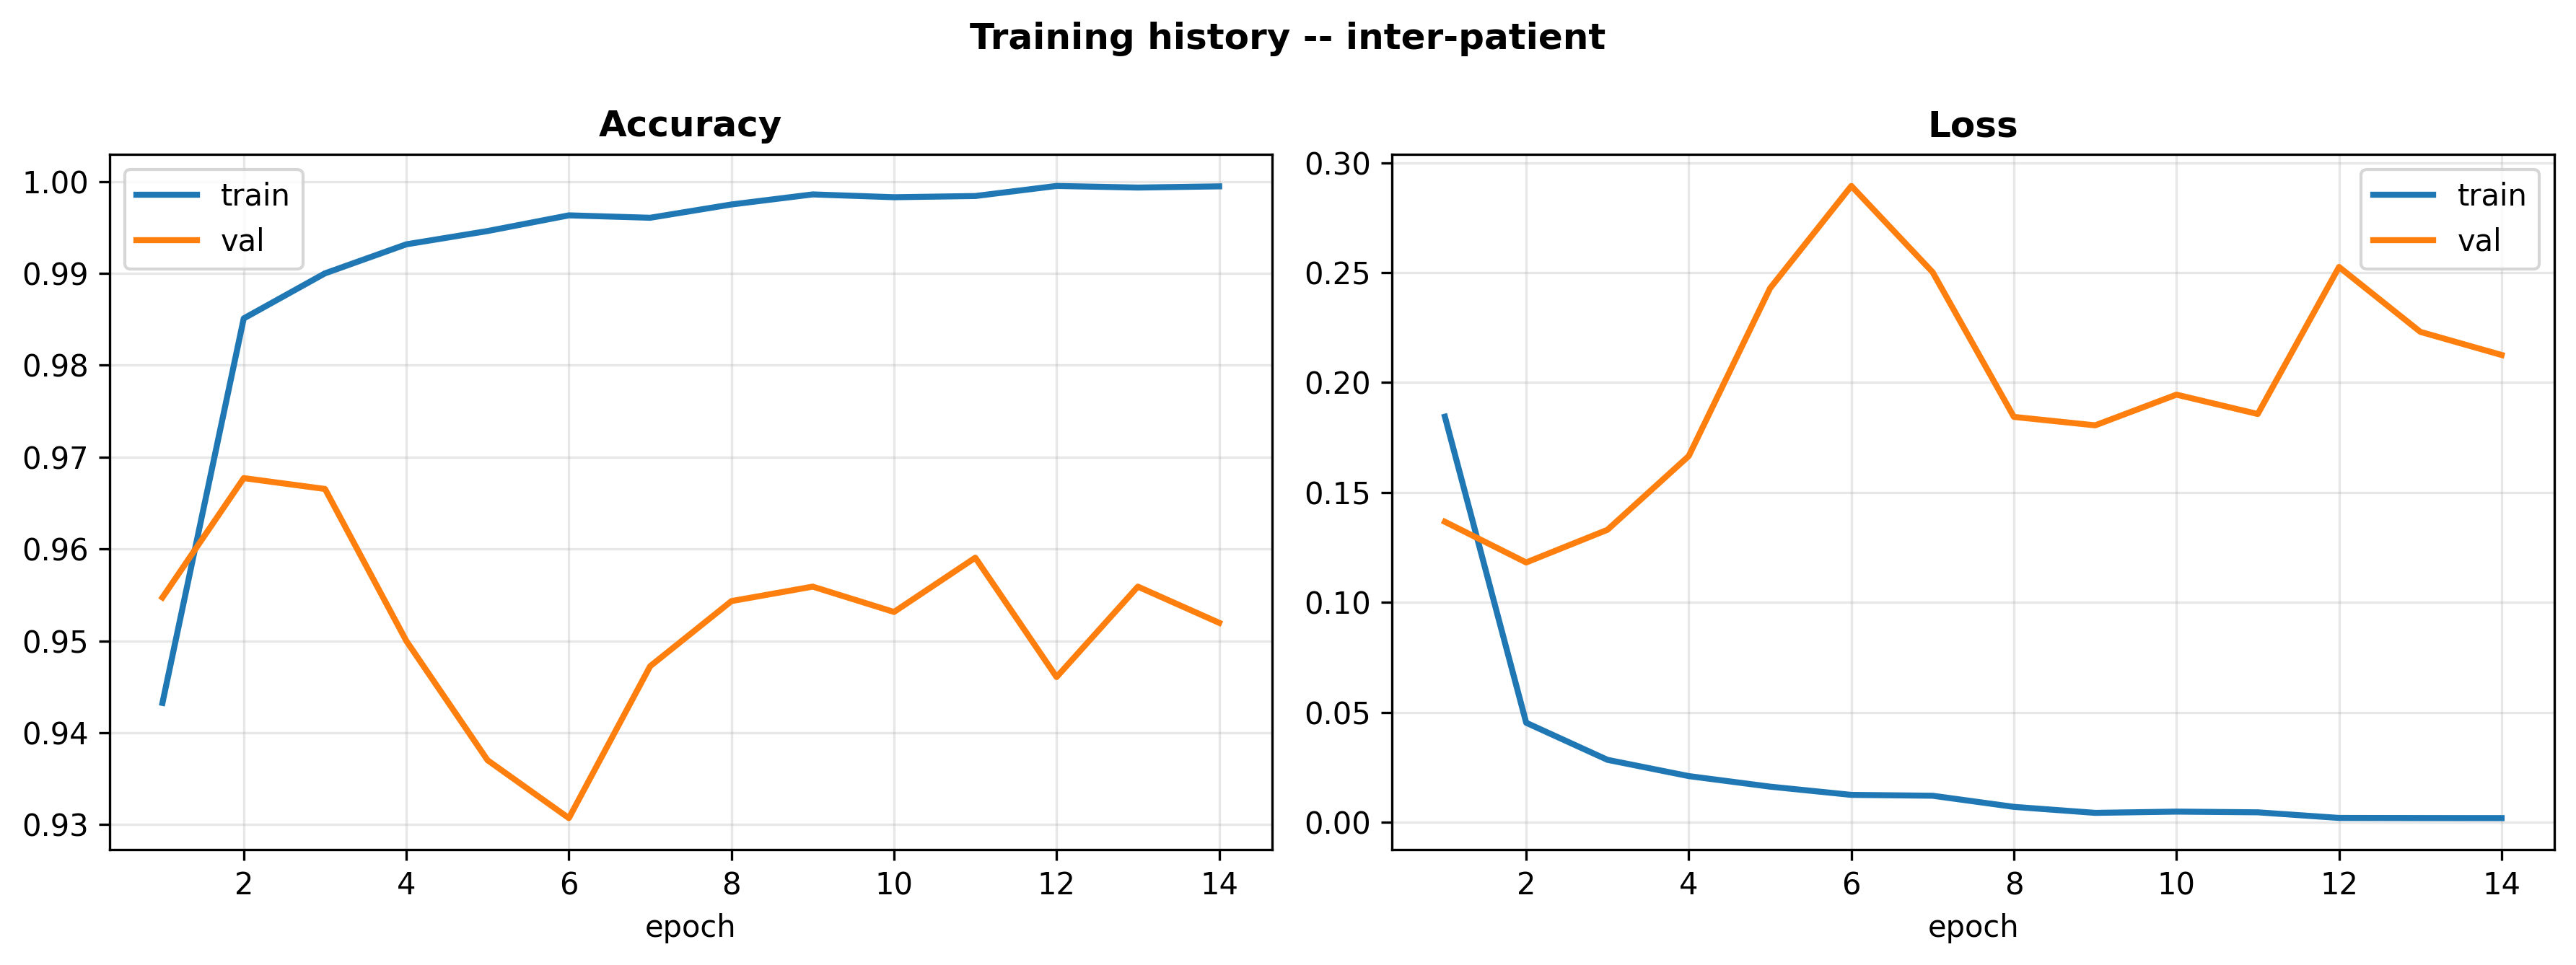
\includegraphics[width=0.95\linewidth]{figures/Inter_Patient/01_training_history.png}
\caption{Training and validation curves for the CNN--BiLSTM--Attention hybrid under the inter-patient protocol}
\label{fig:train_hybrid}
\end{figure}

The hybrid fuses quickly to the training objective: validation accuracy
already exceeds 0.98 in the early epochs while macro-$F_1$ oscillates in the
0.71--0.77 band, and after early stopping at epoch~14 the epoch-2 weights
are recovered. This is the expected behaviour of a high-capacity model: the
capacity is spent recalling patient-specific local waveform details that do
not transfer, and the learning-rate reductions of
\texttt{ReduceLROnPlateau} (at epochs~7 and~12) purchase stability but not
generalisation.

\begin{figure}[!t]
\centering
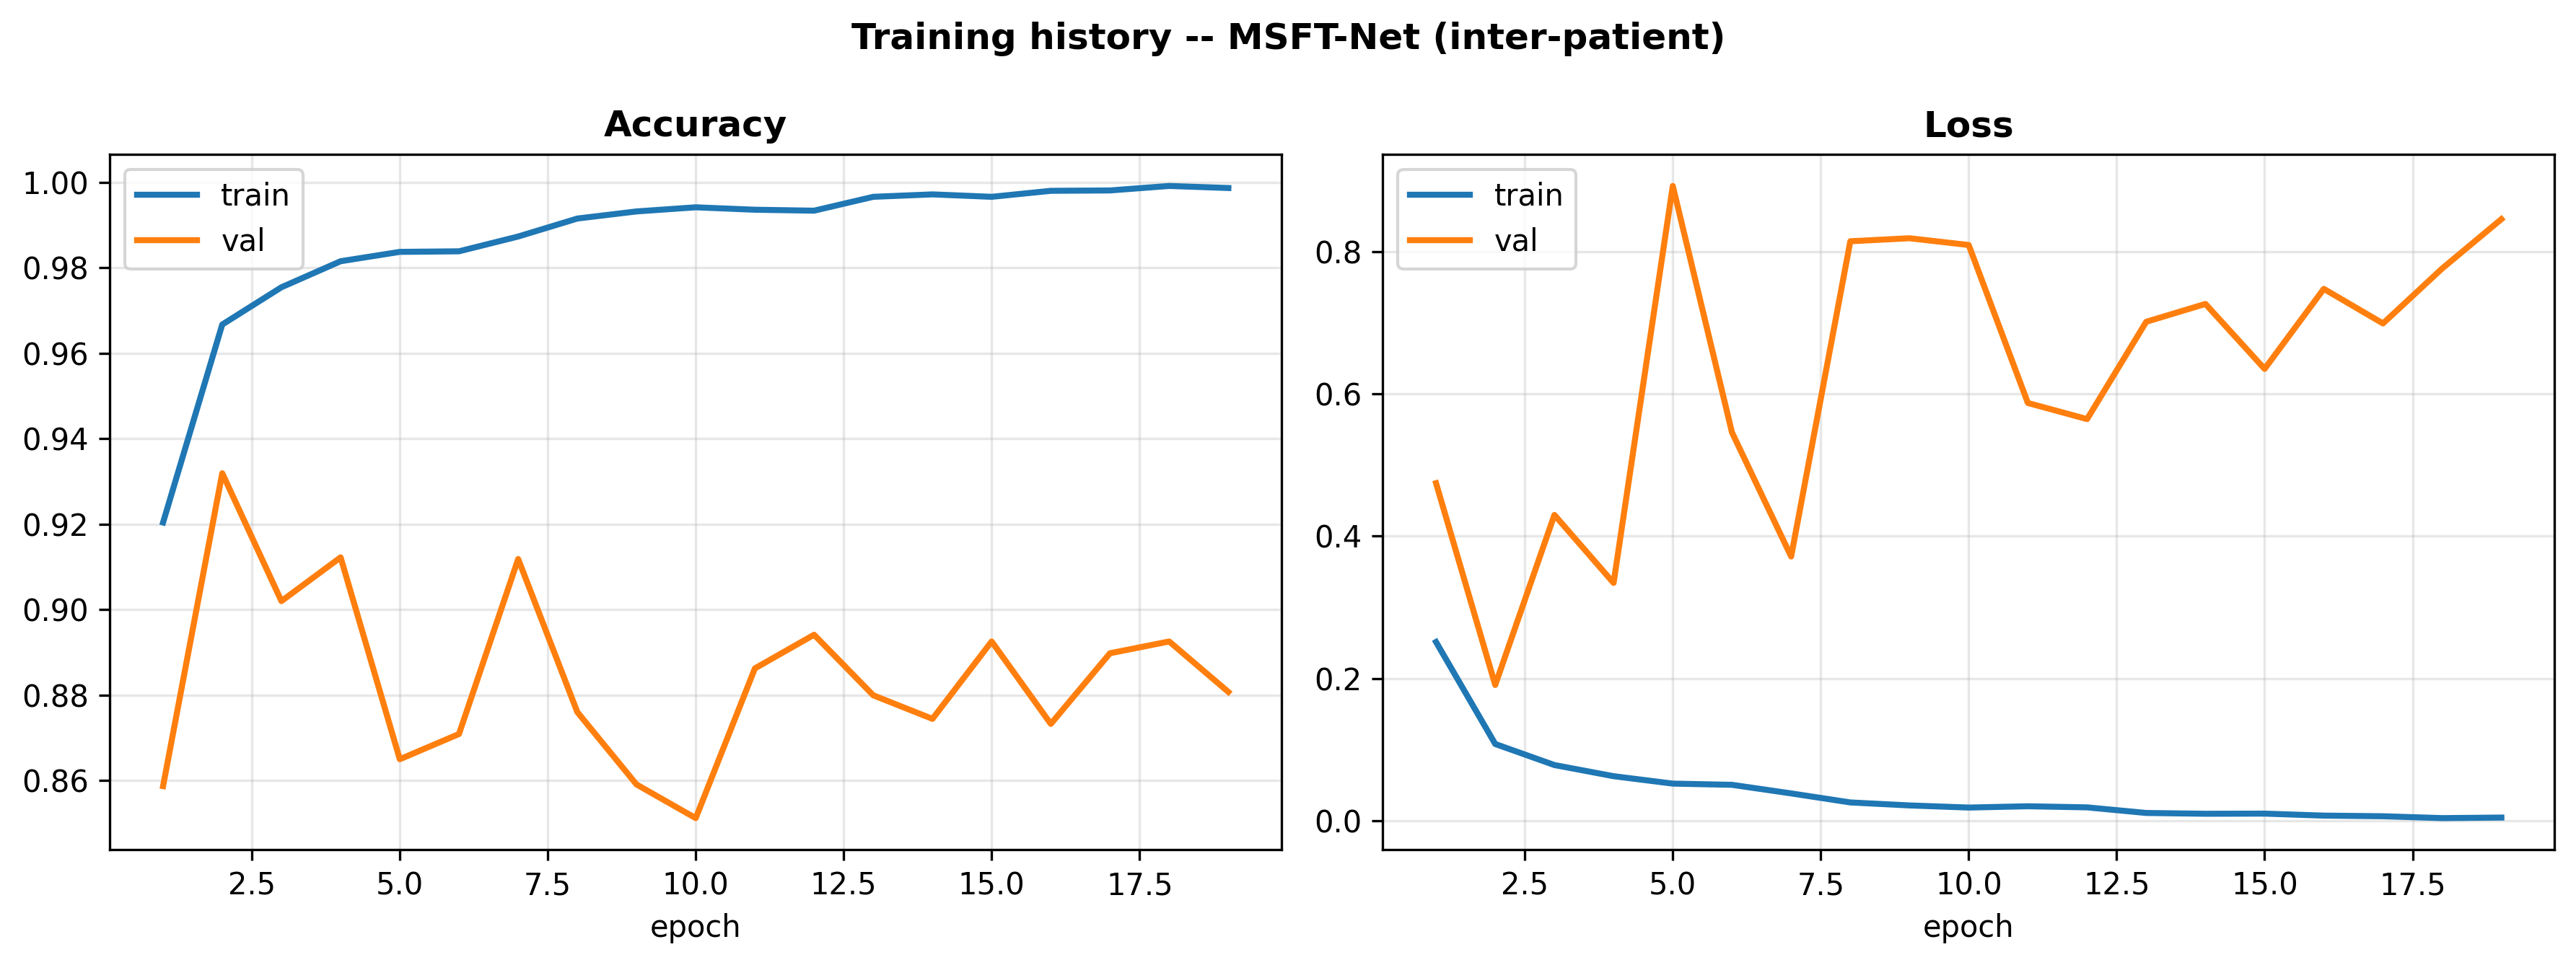
\includegraphics[width=0.95\linewidth]{figures/Inter_Patient/01b_training_history_msft.png}
\caption{Training and validation curves for MSFT-Net under the inter-patient protocol}
\label{fig:train_msft}
\end{figure}

MSFT-Net tells a different story. Its validation curve is higher and less
erratic because of its multi-scale stem and the auxiliary-vector dropout
that breaks up the reliance on convolutions; the patient-specific FiLM
conditioning visibly reduces validation variance. The two curves flank the
central, experimentally found architectural conclusion of this part: for
inter-patient generalisation, a compact convolutional model conditioned on
auxiliary features is much larger in benefit than a much larger recurrent
one, on exactly the metric that matters.

\subsection{Overall Classification Performance}
\label{subsec:overall}

Table~\ref{tab:perclass} reports the per-class precision, recall, and $F_1$
for both models on the identical test beats, and Table~\ref{tab:headtohead}
gives the paired head-to-head comparison with a McNemar significance test.
The hybrid attains an overall accuracy of 0.8200 (95\% CI [0.8120, 0.8278])
and a macro-$F_1$ of 0.7326, whereas MSFT-Net attains 0.8945 (95\% CI
[0.8881, 0.9007]) and a macro-$F_1$ of 0.8725.

\begin{table}[!t]
\centering
\caption{Per-class precision, recall, and $F_1$ on the frozen inter-patient test set for the CNN--BiLSTM--Attention hybrid and MSFT-Net}
\label{tab:perclass}
\begin{tabular}{lrrrrrrr}
\toprule
 & & \multicolumn{3}{c}{CNN--BiLSTM--Attention} & \multicolumn{3}{c}{MSFT-Net} \\
\textbf{Class} & \textbf{Support} & P & R & $F_1$ & P & R & $F_1$ \\
\midrule
N-Normal   & 6{,}047 & 0.8810 & 0.8629 & 0.8718 & 0.9472 & 0.9046 & 0.9254 \\
S-Supra    & 1{,}837 & 0.8618 & 0.7300 & 0.7905 & 0.7827 & 0.8372 & 0.8090 \\
V-Ventri   &   333   & 0.7741 & 0.9159 & 0.8391 & 0.8284 & 0.9279 & 0.8754 \\
F-Fusion   &   388   & 0.6000 & 0.9278 & 0.7287 & 0.8042 & 0.8892 & 0.8446 \\
Q-Unknown  &   507   & 0.3881 & 0.4892 & 0.4328 & 0.8579 & 0.9645 & 0.9081 \\
\midrule
Macro avg  & 9{,}112 & 0.7010 & 0.7852 & 0.7326 & 0.8441 & 0.9047 & 0.8725 \\
Accuracy   & 9{,}112 & \multicolumn{3}{c}{0.8200} & \multicolumn{3}{c}{0.8945} \\
\bottomrule
\end{tabular}
\end{table}

\begin{table}[!t]
\centering
\caption{Paired head-to-head comparison of the two models on identical inter-patient test beats}
\label{tab:headtohead}
\begin{tabular}{lrrr}
\toprule
\textbf{Model} & \textbf{Params} & \textbf{Accuracy} & \textbf{Macro-$F_1$} \\
\midrule
CNN--BiLSTM--Attention & 572{,}358 & 0.8200 & 0.7326 \\
MSFT-Net               & 167{,}090 & 0.8945 & 0.8725 \\
\midrule
McNemar & \multicolumn{3}{c}{$p \approx 0$ (significant)} \\
\bottomrule
\end{tabular}
\end{table}

Table~\ref{tab:perclass} gives a more informative picture than the headline
accuracy. For the hybrid, the fusion class achieves high recall (0.9278) but
poor precision (0.6000), meaning the model readily recognises fusion
morphology but over-predicts it; the $Q$ class is the hybrid's clear weak
point, with an $F_1$ of only 0.4328. Moving to MSFT-Net, per-class
sensitivity improves for N (0.8629~$\rightarrow$~0.9046), S
(0.7300~$\rightarrow$~0.8372), V (0.9159~$\rightarrow$~0.9279), and most
strikingly Q (0.4892~$\rightarrow$~0.9645), at the cost of a small drop in F
recall (0.9278~$\rightarrow$~0.8892) that is more than offset by a large
gain in F precision (0.6000~$\rightarrow$~0.8042). The McNemar test in
Table~\ref{tab:headtohead} verifies that the improvement is not elementary
chance: MSFT-Net fixed many more of the hybrid's errors than it introduced.

Two caveats apply to the $Q$ result. First, $Q$ is supported by only nine
records in the corpus and by a single held-out record in the test set, so
$Q$ sensitivity and precision are de facto single-patient statistics whose
real confidence interval is the between-patient spread, not the binomial
interval computed as if $Q$ had the same statistical support as N/S/V/F.
Second, the $Q$ class is paced, and its separability partly stems from the
presence of paced beats rather than from a general ability to recognise
``unknown'' rhythms. Both caveats are honoured in the AAMI reporting of
Section~\ref{subsec:ec57}.

\begin{figure}[!t]
\centering
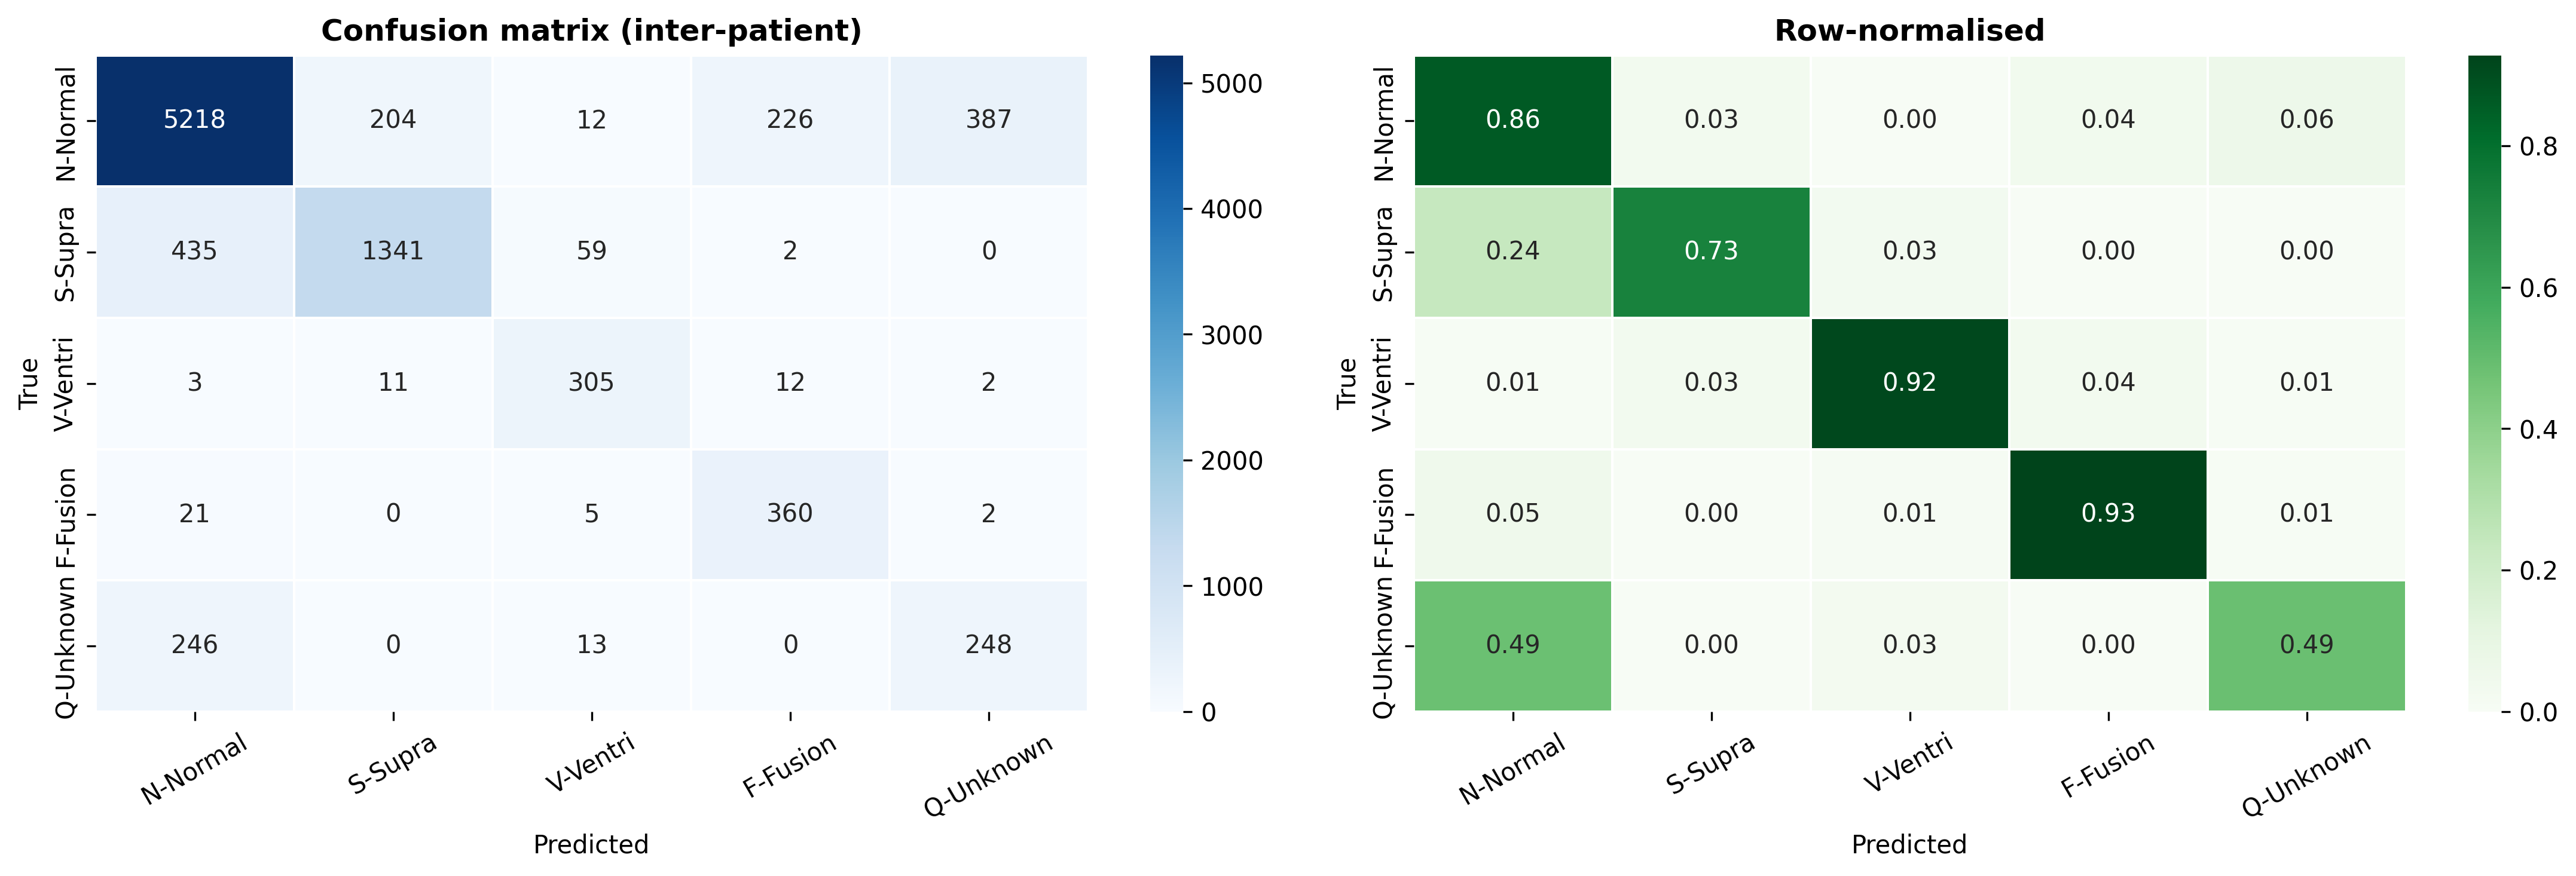
\includegraphics[width=0.95\linewidth]{figures/Inter_Patient/02_confusion_matrix.png}
\caption{Confusion matrix of the CNN--BiLSTM--Attention hybrid on the inter-patient test set}
\label{fig:cm_hybrid}
\end{figure}

\begin{figure}[!t]
\centering
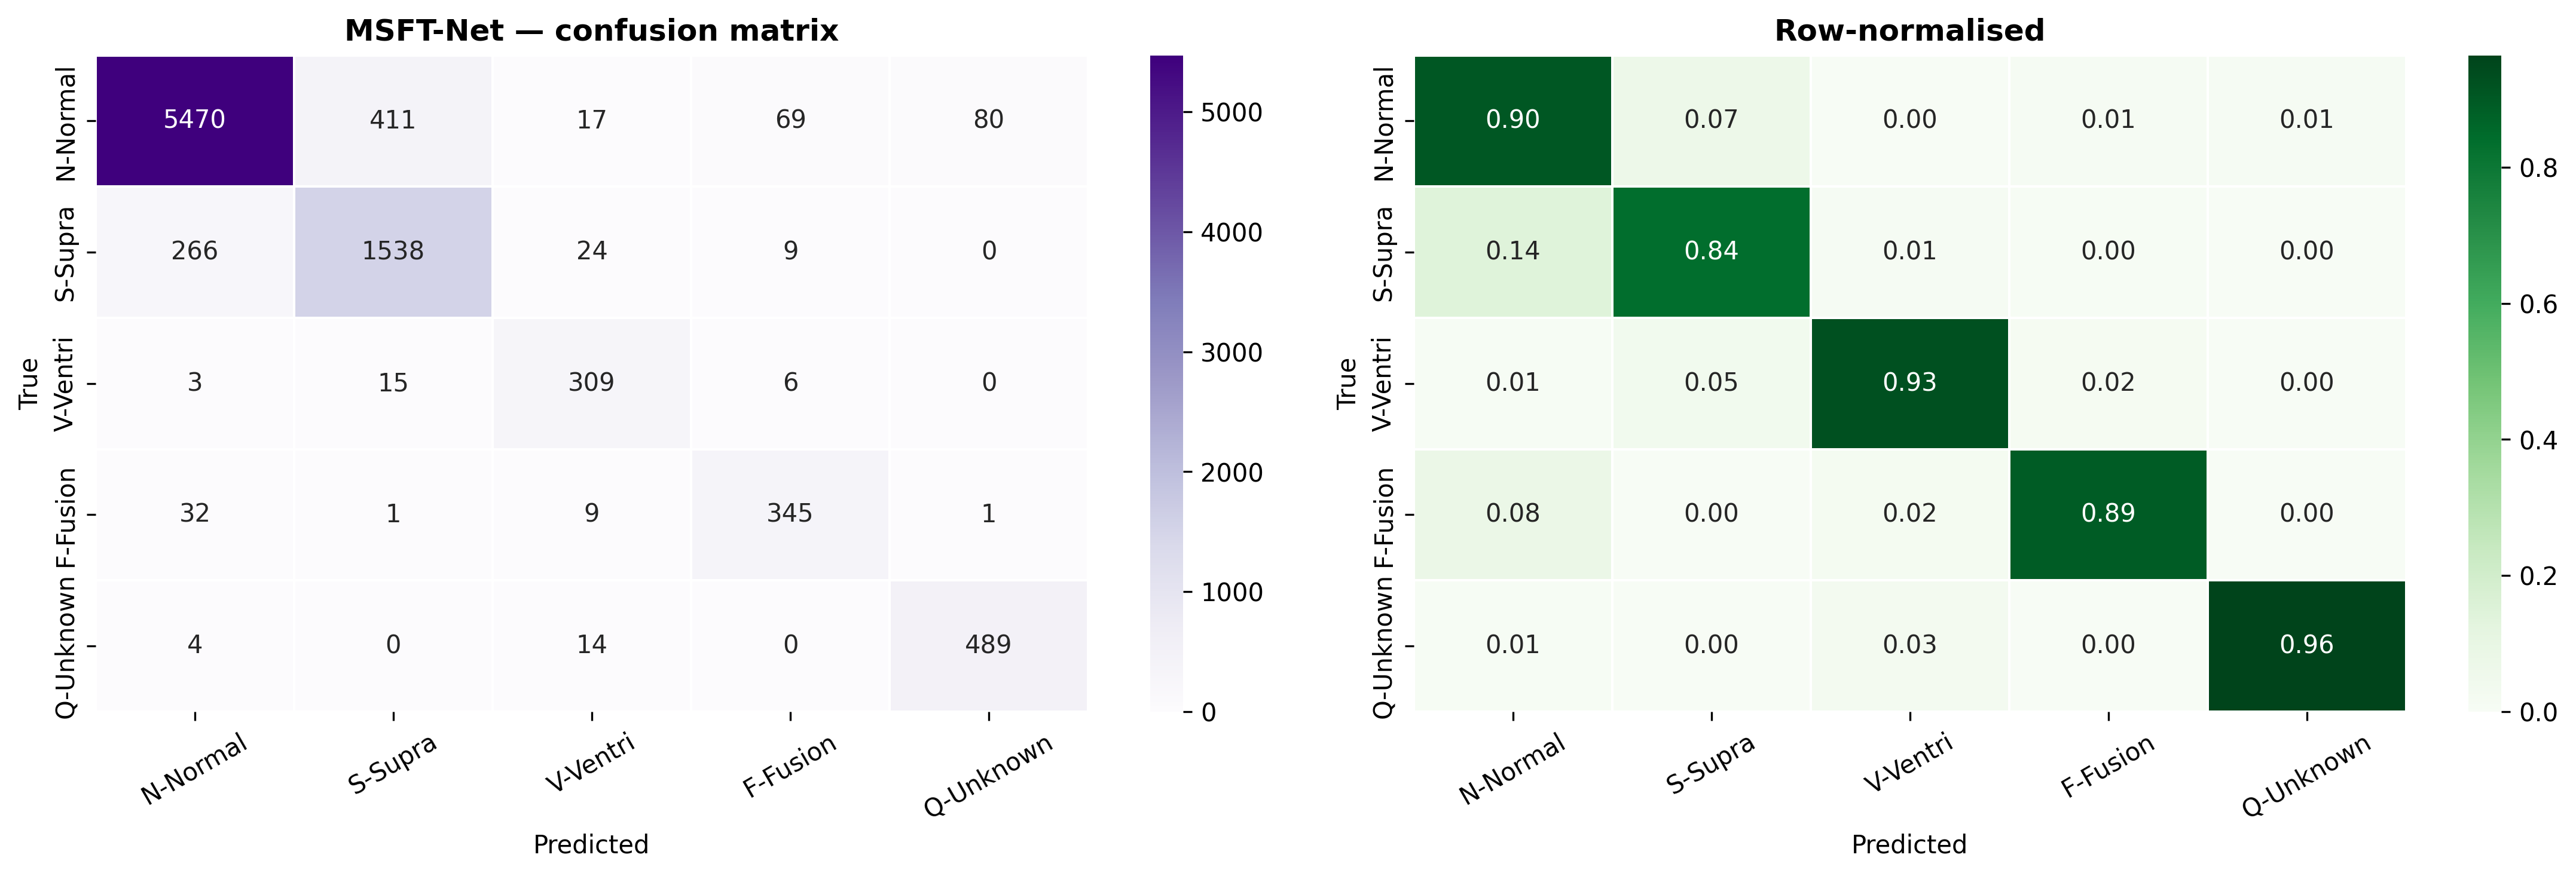
\includegraphics[width=0.95\linewidth]{figures/Inter_Patient/02b_confusion_matrix_msft.png}
\caption{Confusion matrix of MSFT-Net on the same inter-patient test beats}
\label{fig:cm_msft}
\end{figure}

\begin{figure}[!t]
\centering
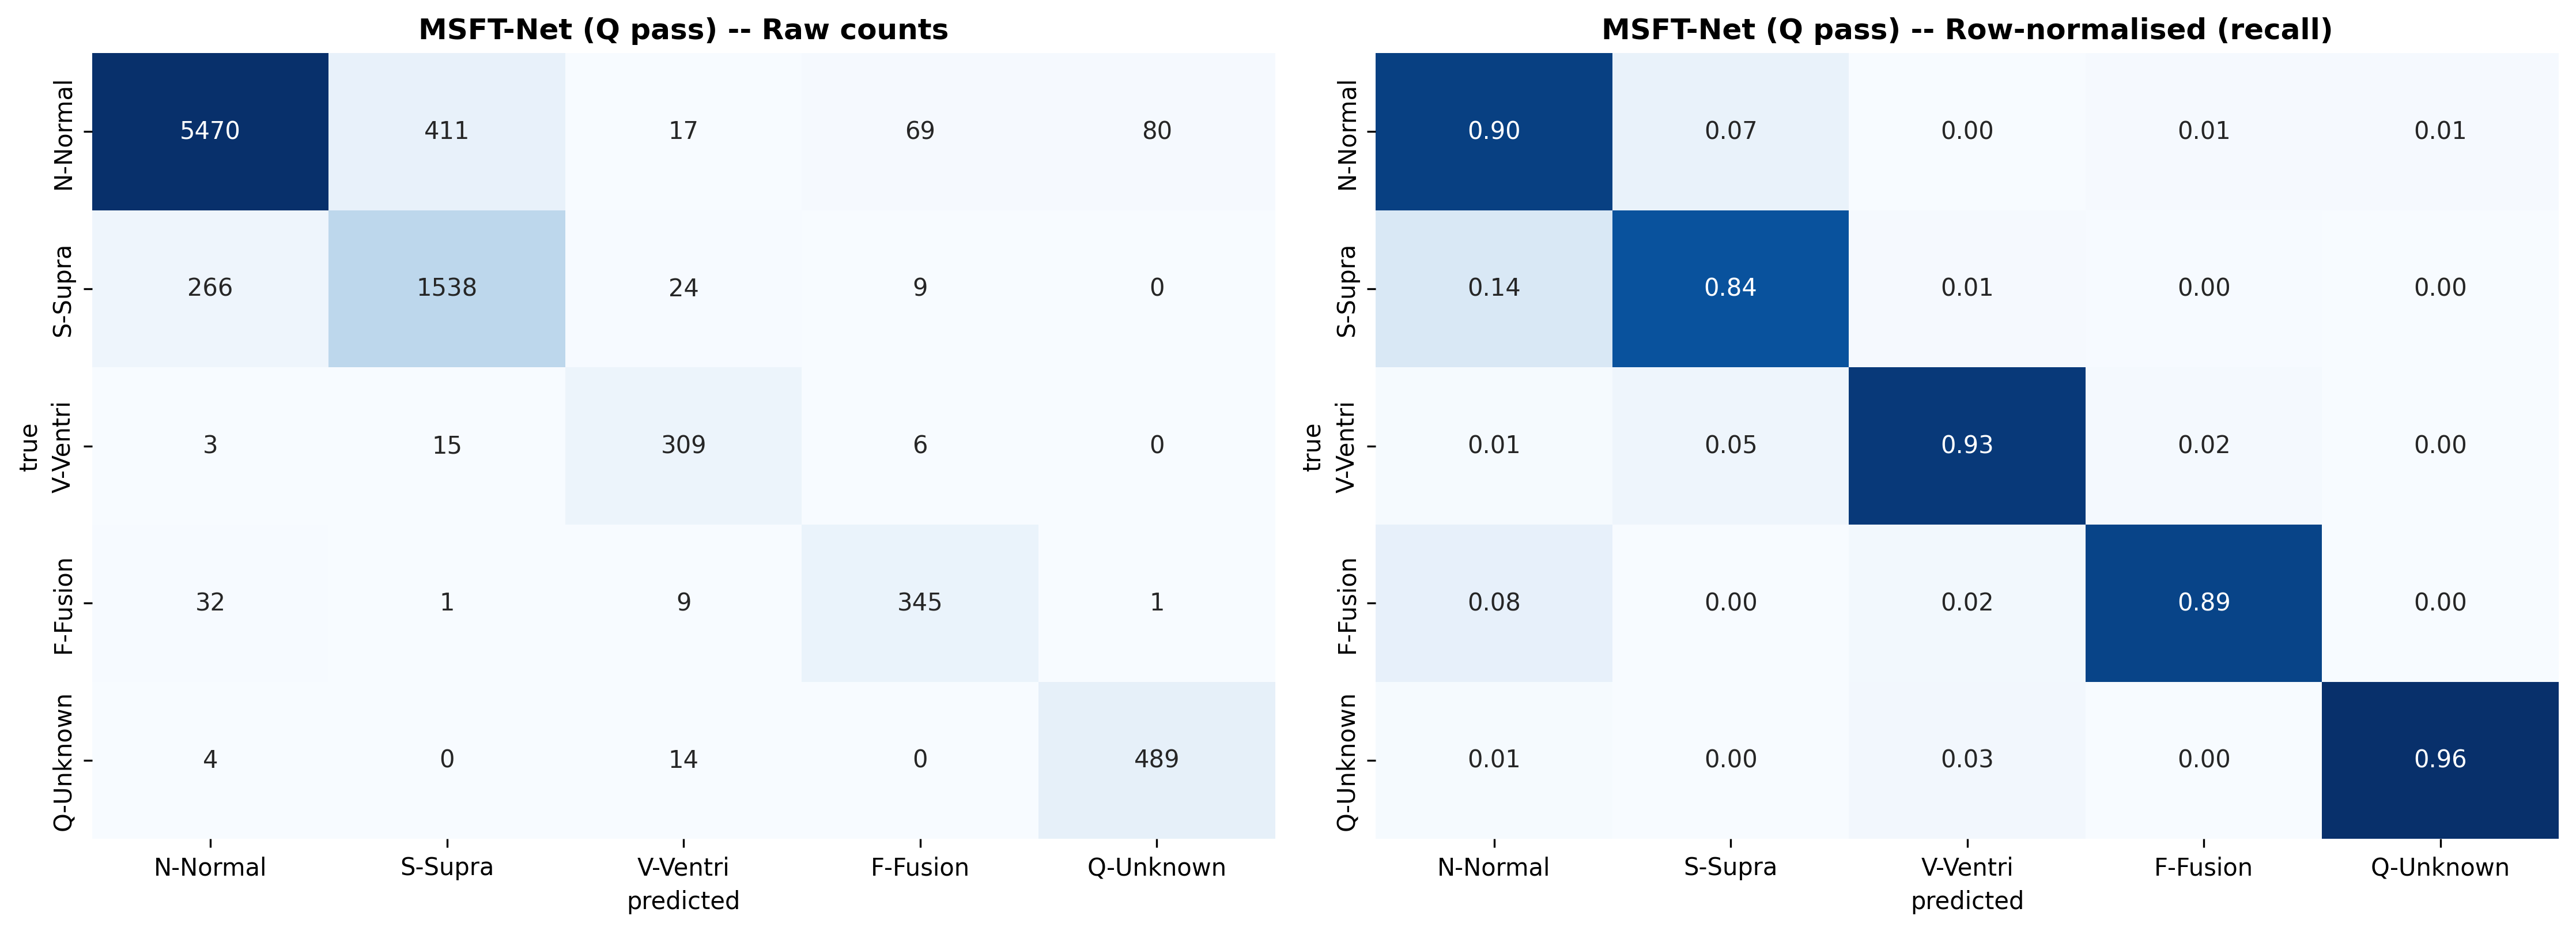
\includegraphics[width=0.95\linewidth]{figures/Inter_Patient/06g_confusion_q_pass.png}
\caption{Confusion structure of the $Q$ class under the pass policy}
\label{fig:cm_qpass}
\end{figure}

The confusion matrices in Figures~\ref{fig:cm_hybrid} and~\ref{fig:cm_msft}
localise the errors. For the hybrid, the two largest symmetric error pairs
among the 1{,}640 misclassifications are N$\leftrightarrow$S (639 beats,
39.0\% of errors) and N$\leftrightarrow$Q (633 beats, 38.6\%). This is a
clinically coherent error structure: supraventricular ectopy is
characterised more by prematurity than by a markedly different QRS shape,
so it is automatically confused with normal beats from patients the model
has never seen, and unseen paced $Q$ beats wander towards the normal
manifold. MSFT-Net's auxiliary features almost eradicate the N$\leftrightarrow$Q
confusion, leaving the genuinely challenging N$\leftrightarrow$S and
N$\leftrightarrow$F boundaries as the major residual error, precisely the
boundaries that human annotators also find most difficult.

\subsection{AAMI EC57 Reporting}
\label{subsec:ec57}

As outlined in EC57, accuracy is dominated by the normal class, so the
clinically relevant statistics are the class sensitivity (Se) and positive
predictivity ($+P$). Gross statistics pooled over all test records are
given in Table~\ref{tab:ec57} for MSFT-Net, together with 95\% Wilson
confidence intervals and the per-class false-positive rate.

\begin{table}[!t]
\centering
\caption{AAMI EC57 gross statistics for MSFT-Net, pooled over all inter-patient test records}
\label{tab:ec57}
\begin{tabular}{lrccc}
\toprule
\textbf{Class} & \textbf{$n$} & \textbf{Se [95\% CI]} & \textbf{$+P$ [95\% CI]} & \textbf{FPR} \\
\midrule
N-Normal  & 6{,}047 & 0.9046 [0.897, 0.912] & 0.9472 [0.941, 0.953] & 0.0995 \\
S-Supra   & 1{,}837 & 0.8372 [0.820, 0.853] & 0.7827 [0.764, 0.800] & 0.0587 \\
V-Ventri  &   333   & 0.9279 [0.895, 0.951] & 0.8284 [0.787, 0.863] & 0.0073 \\
F-Fusion  &   388   & 0.8892 [0.854, 0.917] & 0.8042 [0.764, 0.839] & 0.0096 \\
Q-Unknown &   507   & 0.9645 [0.945, 0.977] & 0.8579 [0.827, 0.884] & 0.0094 \\
\bottomrule
\end{tabular}
\end{table}

The EC57 view in Table~\ref{tab:ec57} is the most defensible statement of
clinical performance. Ventricular ectopy, the class whose miss carries the
highest risk, is detected at Se 0.9279 with a false-positive rate of only
0.0073, and fusion beats at Se 0.8892 with FPR 0.0096. The normal class has
the highest FPR (0.0995) simply because it is the standard against which
the minority classes are discriminated. The gross statistics are dominated
by the longest records, so the notebook also computes record-averaged
statistics that treat all patients equally; the two views agree closely for
N and S but differ for V, F, and Q, reflecting the scarce number of records
supporting those classes. It is the between-patient variance, not the
pooled count, that constitutes the largest unknown uncertainty about the
minority classes.

\subsection{ROC, Precision--Recall, and Achievable Operating Points}
\label{subsec:roc}

Figure~\ref{fig:roc_pr} presents the one-versus-rest ROC and
precision--recall curves, and Table~\ref{tab:recallfloor} reports the
precision achievable at fixed recall floors, the quantity a clinician
actually cares about when a minimum detection rate is mandated.

\begin{figure}[!t]
\centering
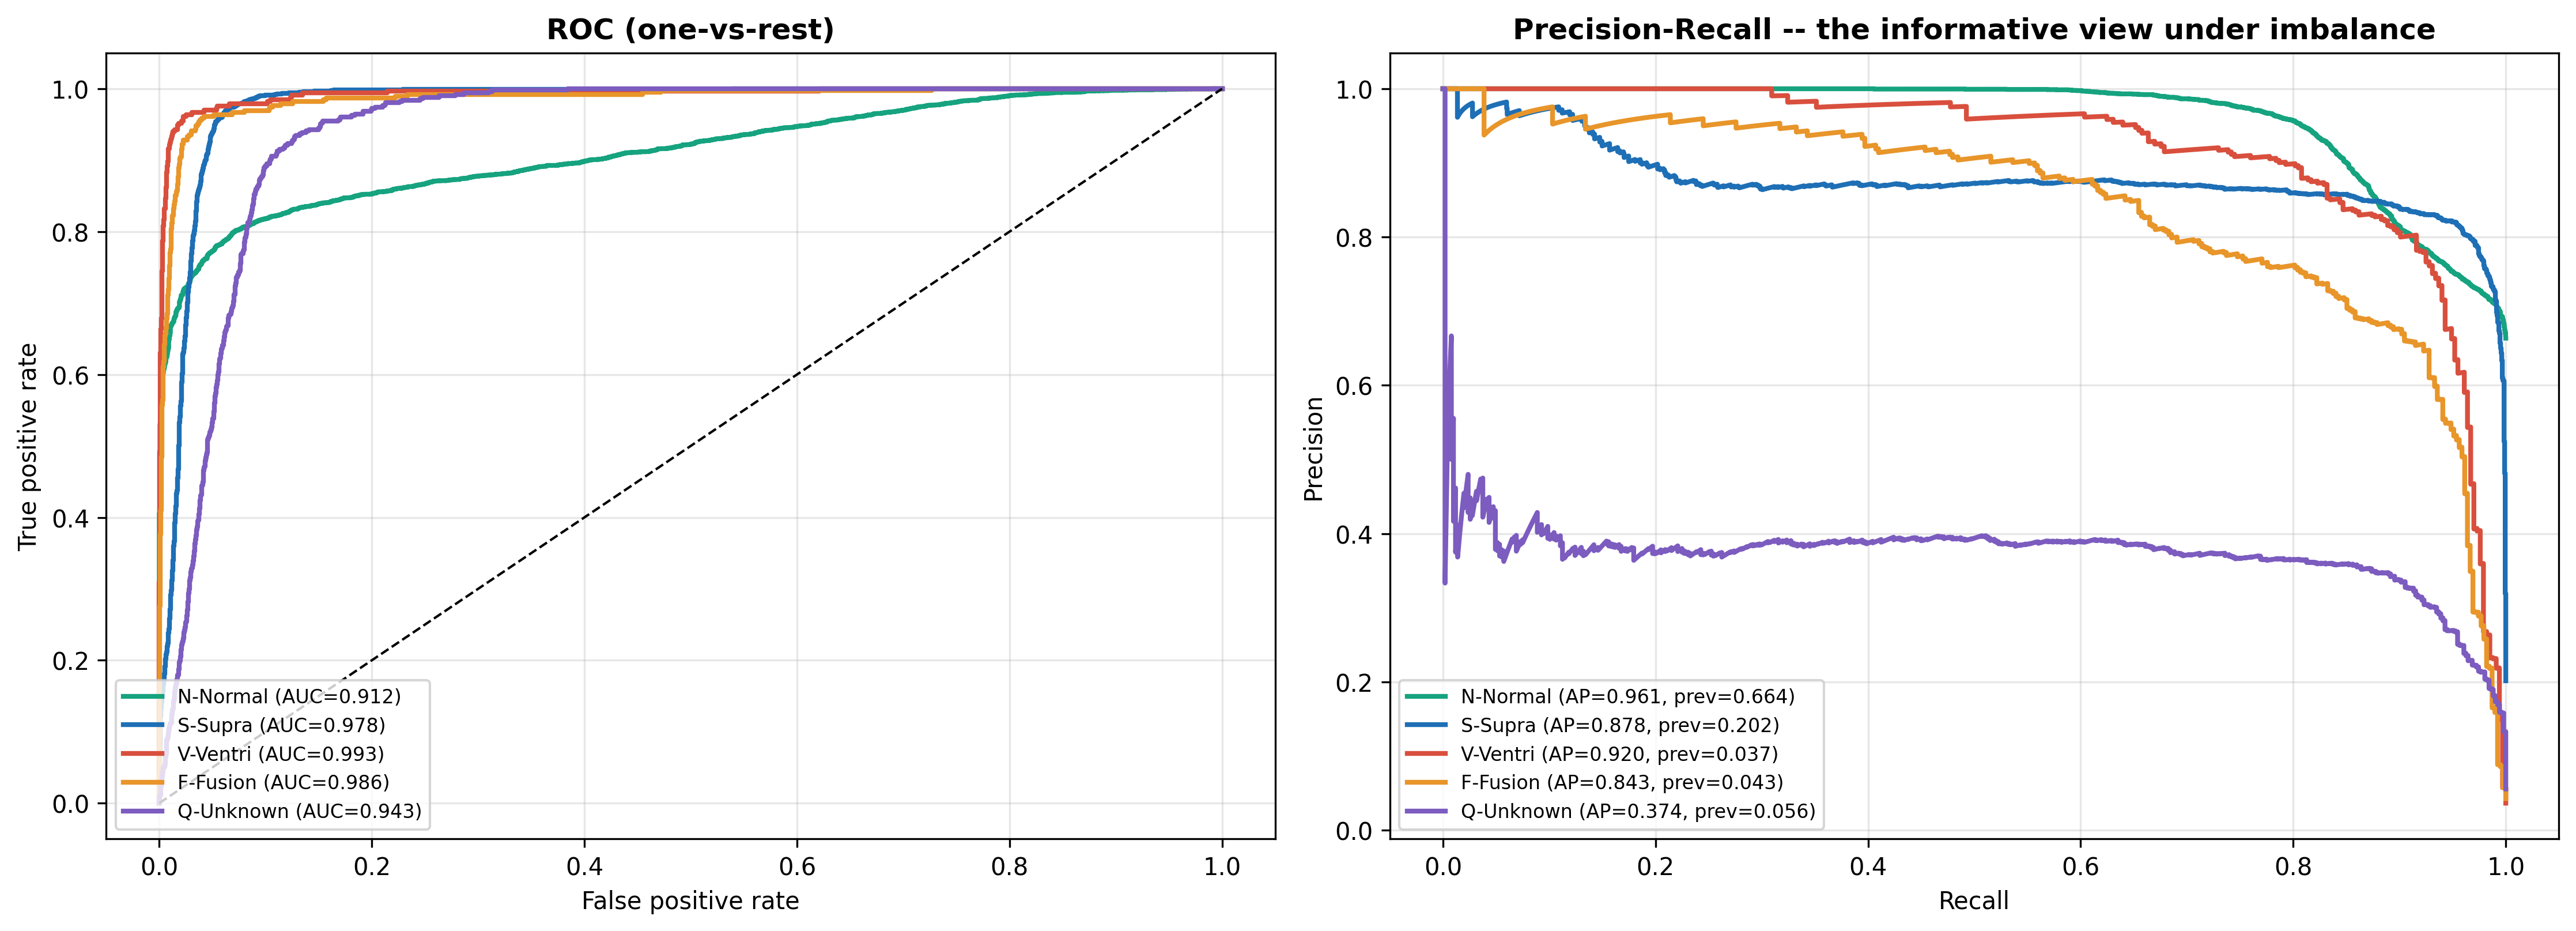
\includegraphics[width=0.95\linewidth]{figures/Inter_Patient/03_roc_pr_curves.png}
\caption{One-versus-rest ROC (left) and precision--recall (right) curves for all five classes under the inter-patient protocol}
\label{fig:roc_pr}
\end{figure}

\begin{table}[!t]
\centering
\caption[Precision achievable at fixed recall floors for the hybrid model]{Precision achievable at fixed recall floors for the CNN--BiLSTM--Attention hybrid}
\label{tab:recallfloor}
\begin{tabular}{lcc}
\toprule
\textbf{Class} & \textbf{Precision @ Recall$\geq$0.95} & \textbf{Precision @ Recall$\geq$0.99} \\
\midrule
N-Normal  & 0.7534 & 0.7097 \\
S-Supra   & 0.8206 & 0.7259 \\
V-Ventri  & 0.6632 & 0.2316 \\
F-Fusion  & 0.5411 & 0.1591 \\
Q-Unknown & 0.2696 & 0.1815 \\
\bottomrule
\end{tabular}
\end{table}

The difference between the ROC and PR panels of Figure~\ref{fig:roc_pr} is
the single most important reason not to present ROC-AUC alone for this
problem: it is easy to obtain a high ROC-AUC when the negative class is
large, but Table~\ref{tab:recallfloor} shows what actually happens when a
fixed recall is demanded. To detect 99\% of true $V$ beats the model will
only accept a precision of 0.2316, and for $F$ and $Q$ the attainable
precision is no better than 0.16 and 0.19 respectively. In deployment terms,
a mandate to ``catch almost every ventricular beat'' is paid for in false
alarms: $S$ is good and cheap, $N$ is bad and costly for the rare-class
false-alarm rate. The operating point of this system must therefore be
justified class by class, not only against the reassuring ROC curves but
against the recall-floor table.

\subsection{Targeted Fusion-Beat Handling}
\label{subsec:fbeat}

The classic failure mode of AAMI classifiers is the fusion class, which is
a collection of beats that mix a normal and a ventricular depolarisation
within a single beat. A staged intervention (global-average pooling,
$F$-specific augmentation, $F/V$ hard-negative mining, and auxiliary
$F$-vs-$N$ / $F$-vs-$V$ losses) was studied in isolation, as shown in
Table~\ref{tab:fablation} and Figures~\ref{fig:f_improvement}
and~\ref{fig:f_destination}.

\begin{table}[!t]
\centering
\caption{Focused F-beat ablation ($A0$--$A5$), each arm adding one component to the previous}
\label{tab:fablation}
\begin{tabular}{lccccc}
\toprule
\textbf{Configuration} & \textbf{F Se} & \textbf{F $+P$} & \textbf{$F_1$-F} & \textbf{Accuracy} & \textbf{Macro-$F_1$} \\
\midrule
$A0$ baseline (attention+focal)   & 0.6469 & 0.7404 & 0.6905 & 0.7886 & 0.6690 \\
$A1$ + GAP pooling                & 0.7423 & 0.8276 & 0.7826 & 0.8293 & 0.7664 \\
$A2$ + F augmentation             & 0.1469 & 0.8382 & 0.2500 & 0.8540 & 0.6677 \\
$A3$ + F/V hard negatives         & 0.8041 & 0.8691 & 0.8353 & 0.8612 & 0.7994 \\
$A4$ + F auxiliary loss           & 0.7268 & 0.7899 & 0.7570 & 0.8300 & 0.7377 \\
$A5$ final (targeted, no focal)   & 0.6546 & 0.8439 & 0.7373 & 0.8628 & 0.8049 \\
\bottomrule
\end{tabular}
\end{table}

\begin{figure}[!t]
\centering
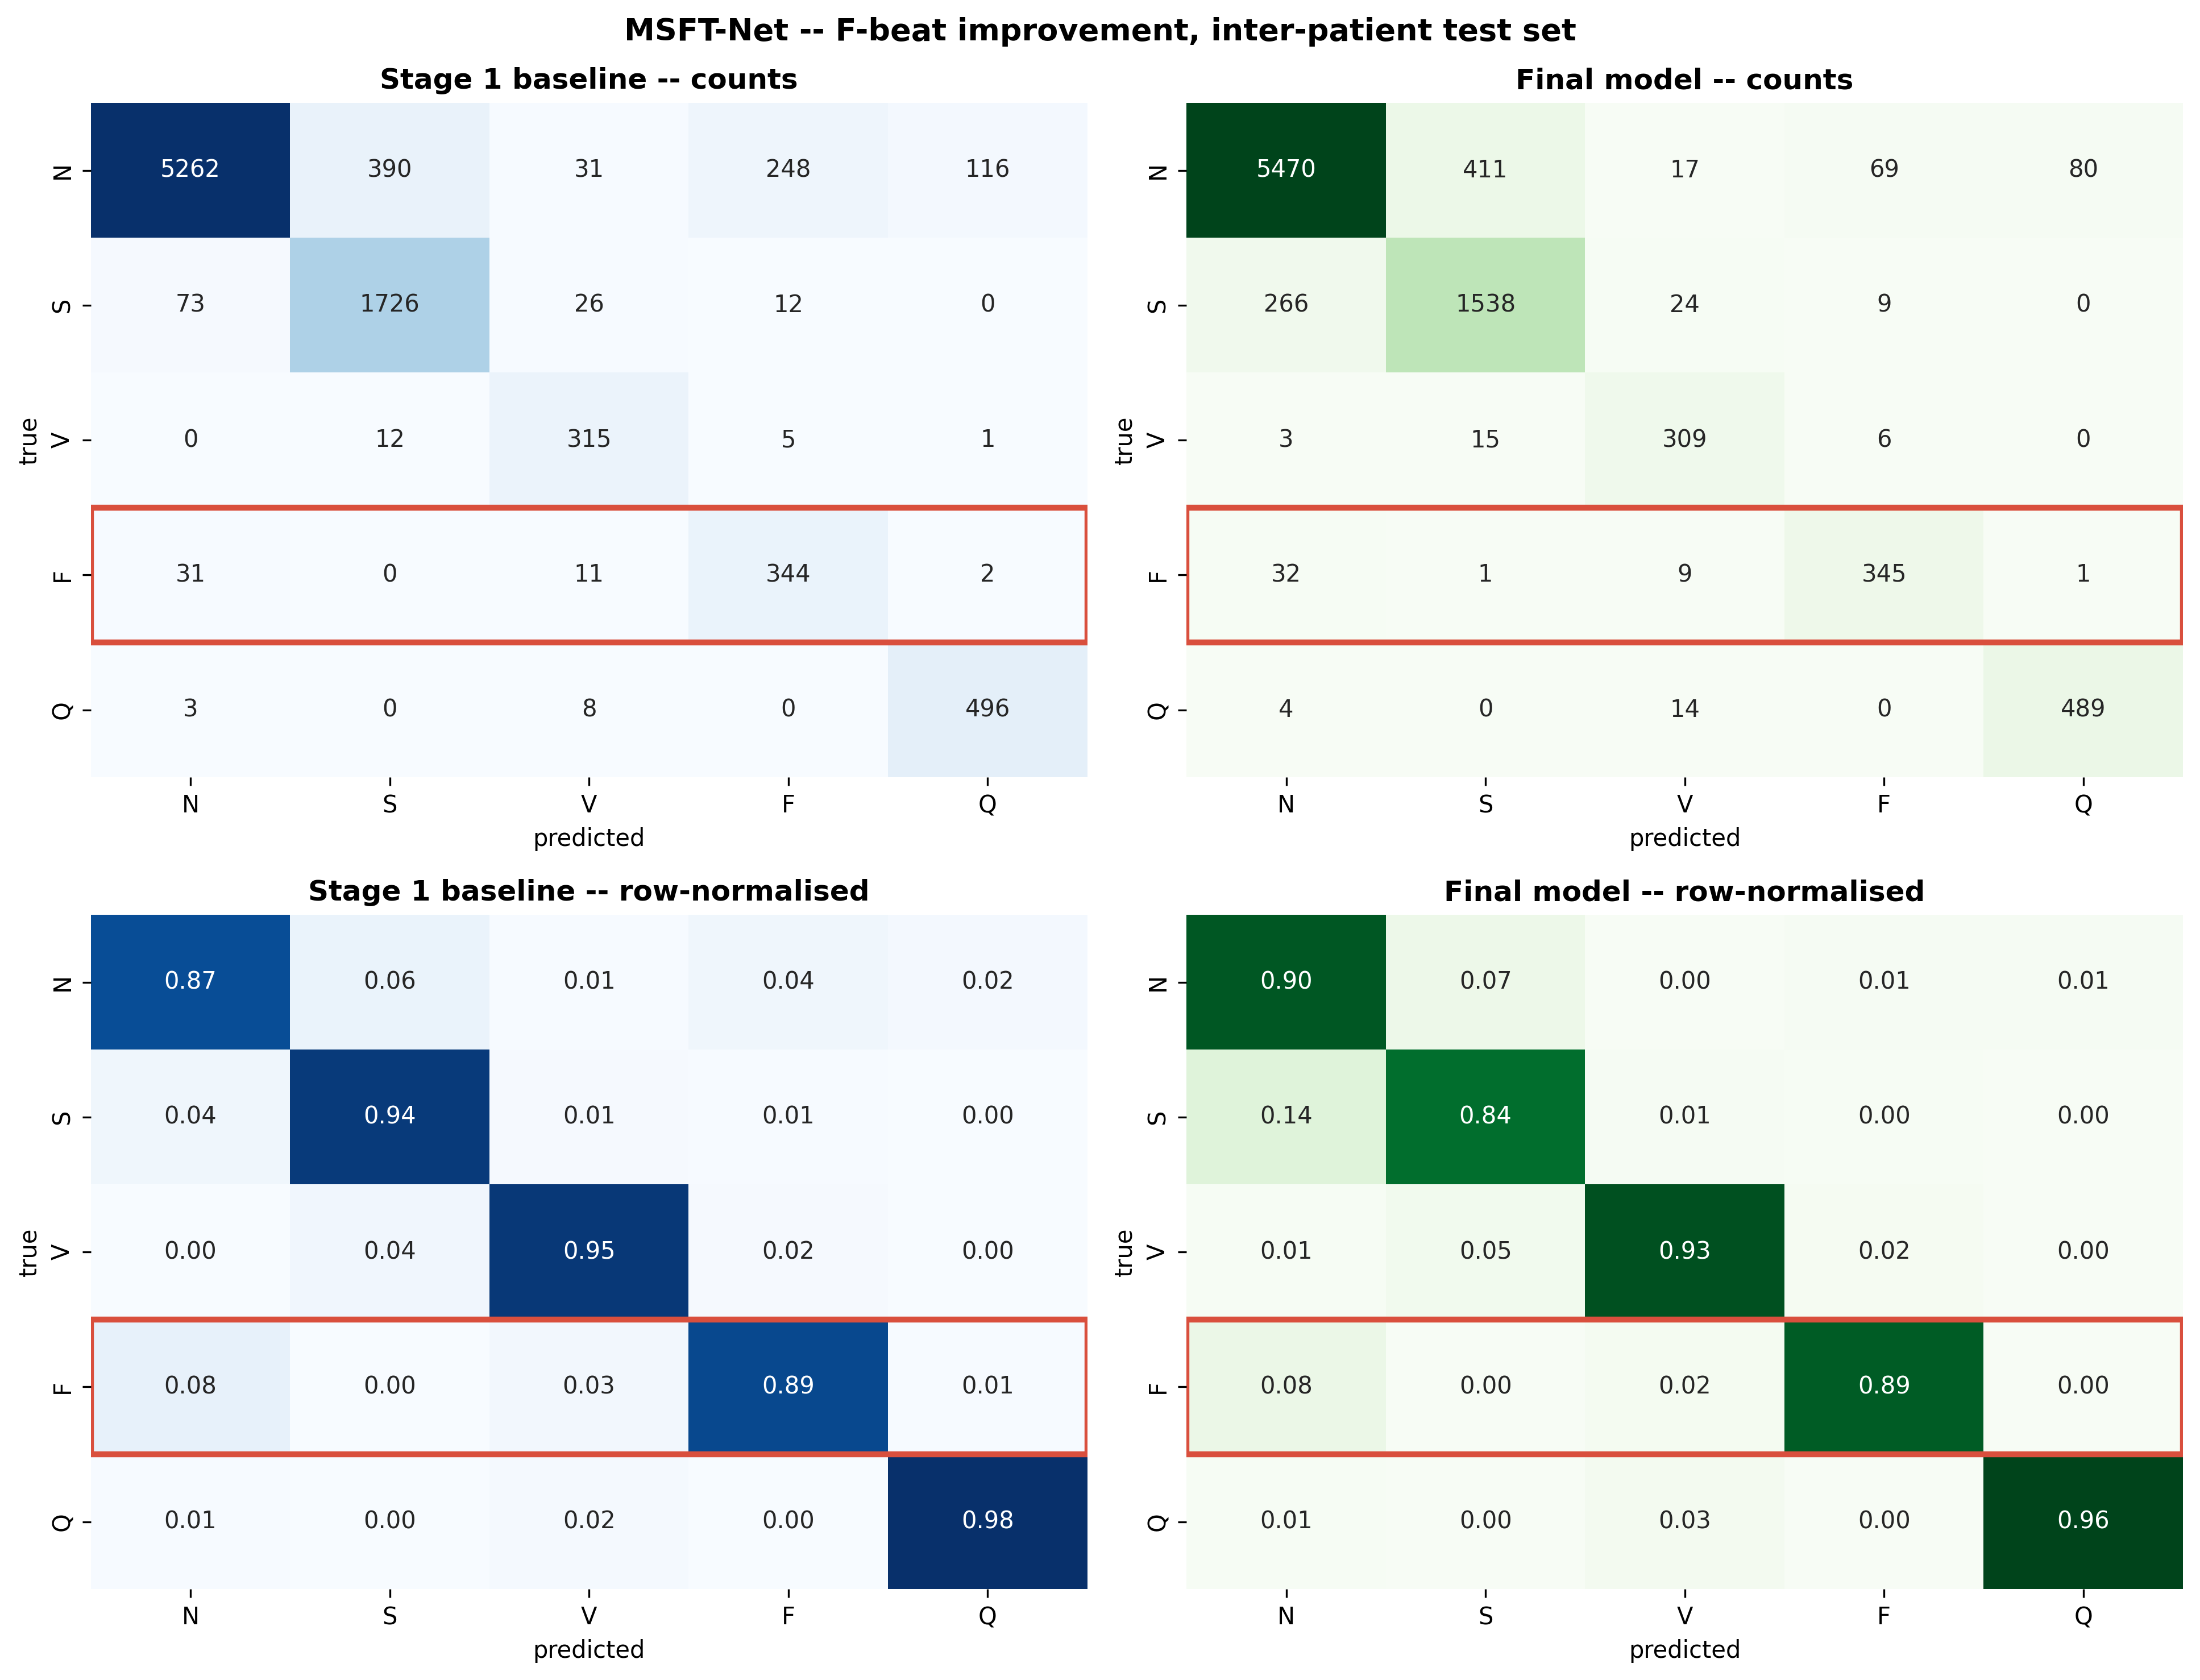
\includegraphics[width=0.95\linewidth]{figures/Inter_Patient/09_f_improvement_confusion.png}
\caption{Confusion structure of the fusion class before and after the targeted improvements}
\label{fig:f_improvement}
\end{figure}

\begin{figure}[!t]
\centering
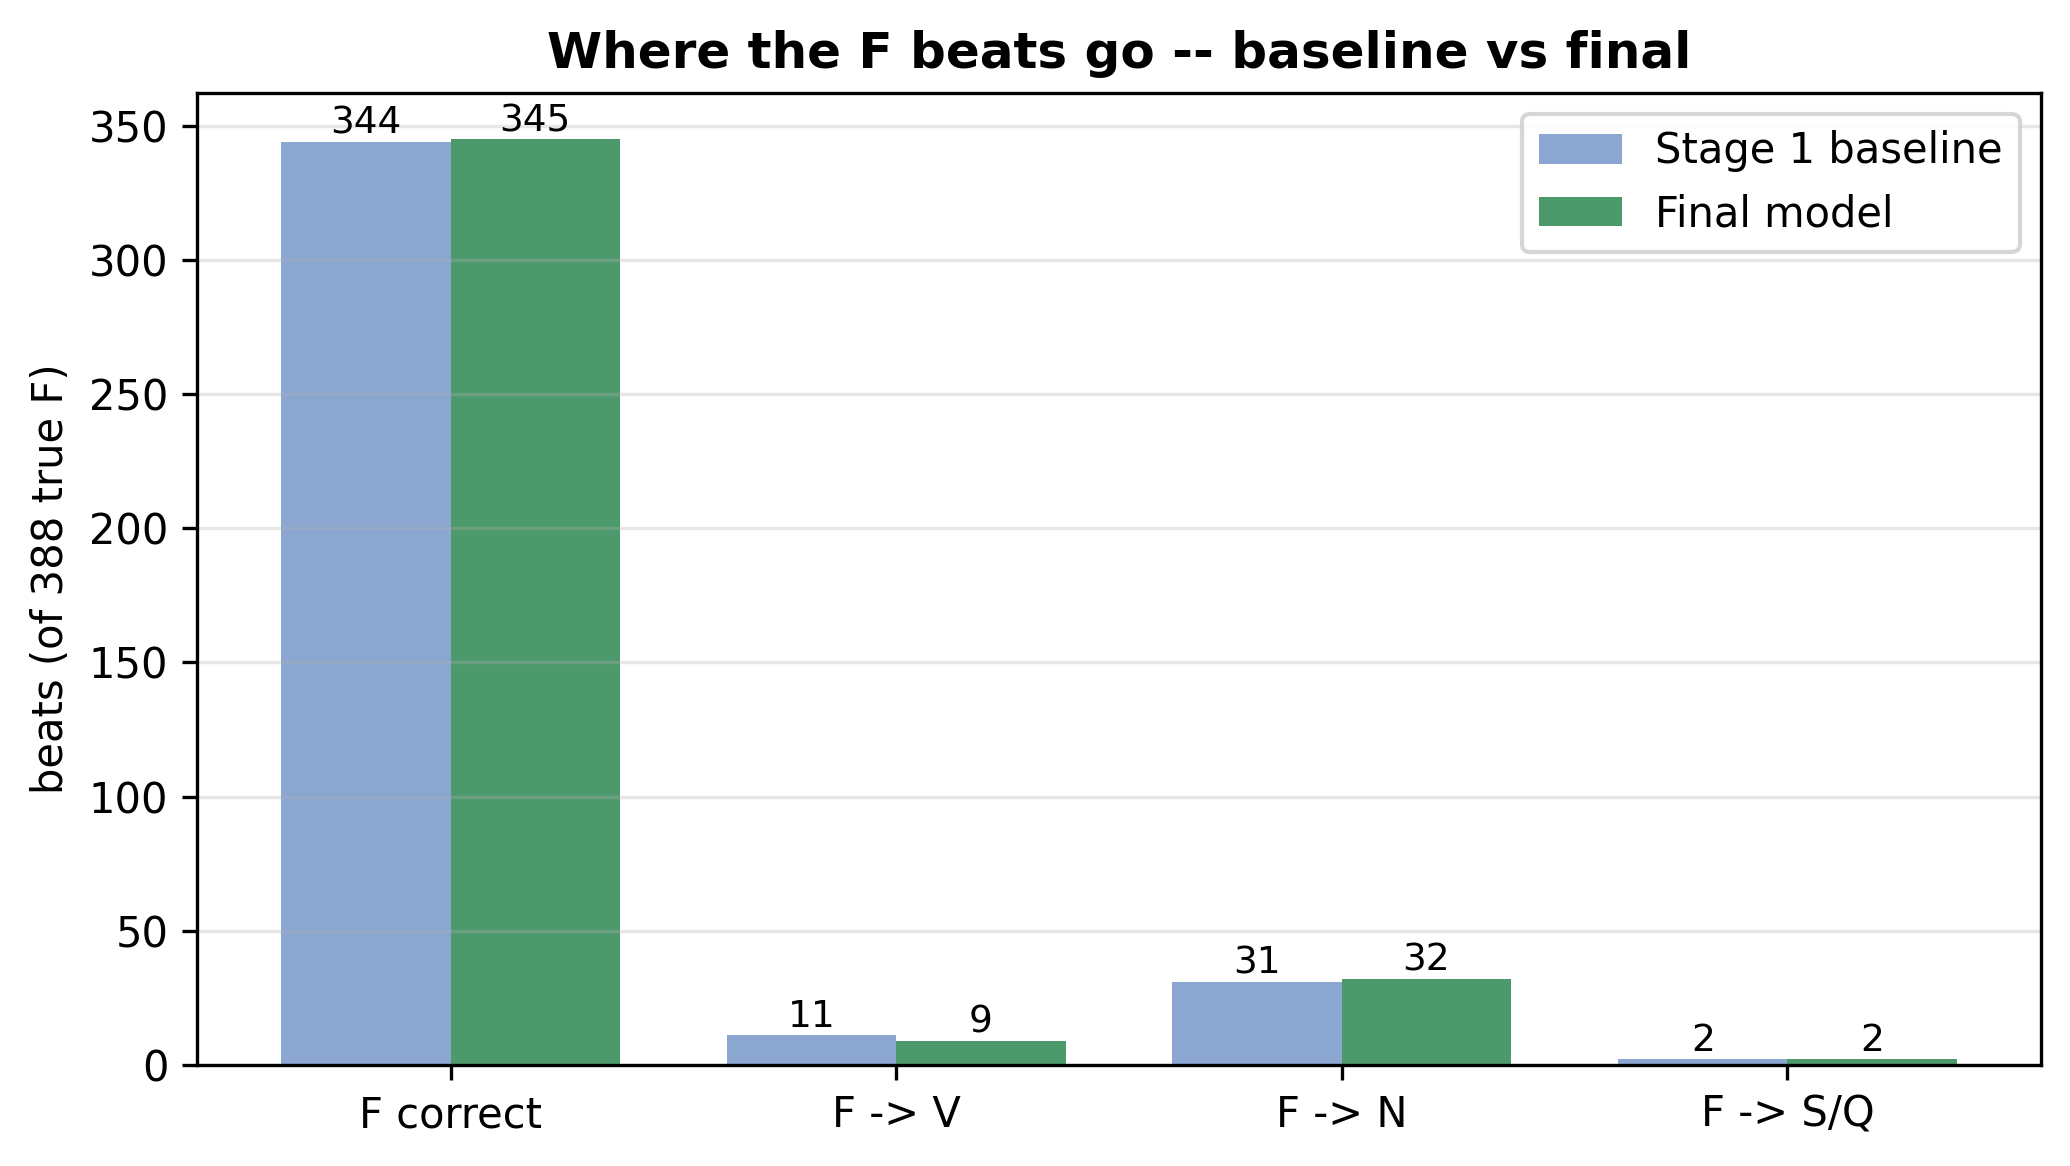
\includegraphics[width=0.95\linewidth]{figures/Inter_Patient/09b_f_destination_comparison.png}
\caption{Destination of the 388 true fusion beats under the baseline and the improved model}
\label{fig:f_destination}
\end{figure}

\begin{figure}[!t]
\centering
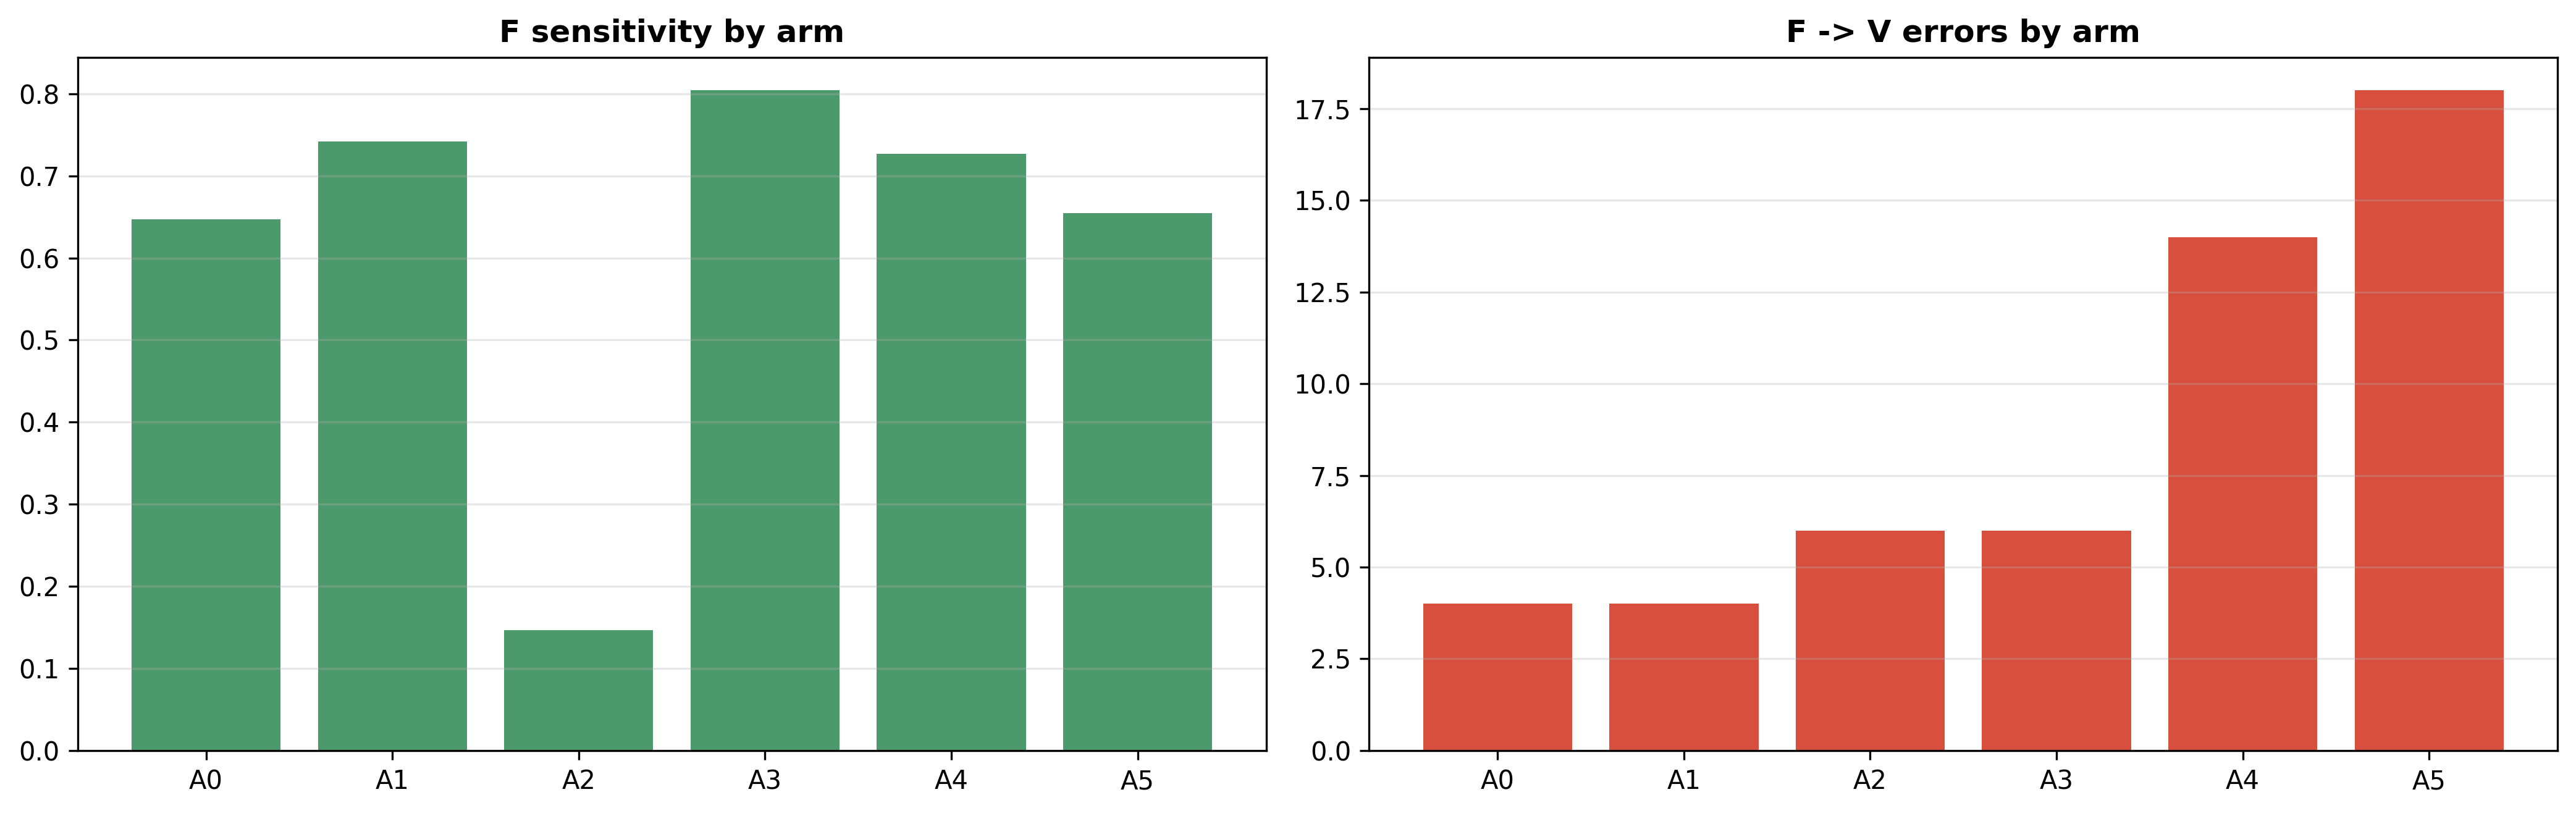
\includegraphics[width=0.95\linewidth]{figures/Inter_Patient/10_f_ablation.png}
\caption{Per-class effects of the fusion-beat ablation arms}
\label{fig:f_ablation}
\end{figure}

Table~\ref{tab:fablation} is cautionary: the naive first inclination,
making ``aggressive'' additional augmentations for the rare $F$ class ($A2$),
is the worst arm for fusion recall, because synthetic $F$ perturbations land
near the normal manifold and train the model to route ambiguous beats to
$N$; $F$ recall collapses to 0.1469 even while overall accuracy is still
rising. This is a textbook example of why accuracy alone must not be used
to judge such interventions. The component that is correctly functioning is
hard-negative mining ($A3$): mining the confusable $V$ and $N$ neighbours
of $F$ raises $F$ $F_1$ to 0.8353. As Figure~\ref{fig:f_improvement} shows,
the net gain is in precision: the improved model stops labelling true $N$
and $V$ beats as $F$ (the most harmful error for fusion precision) while
preserving virtually all of its recall.

A stand-alone probability-calibration and decision-threshold experiment was
also run to push fusion $F_1$ further. Temperature scaling with $T = 3.46$
fitted on the validation set decreased the expected calibration error from
0.0672 to 0.0222 and improved validation $F_1$, but this operating point did
not carry over to the test set: test macro-$F_1$ fell from 0.6768 to 0.6291
and $F$ recall from 0.8918 to 0.4536. This is reported as a negative result
for thresholds learned on validation patients. Because decision thresholds
are expensive to tune properly and transfer poorly across patient cohorts,
all models above are reported at their untuned argmax point rather than at
a tuned threshold.

\subsection{Ablation Study}
\label{subsec:ablation}

Table~\ref{tab:ablation} reports the unified twelve-arm ablation, in which
each arm removes one component and is compared with the full reference model
by macro-$F_1$ with a Holm-corrected McNemar test. All twelve arms were
retrained from scratch under one identical, fixed training budget so that
they are directly comparable with one another; because this budget differs
from the early-stopping schedule used for the headline runs of
Tables~\ref{tab:perclass} and~\ref{tab:headtohead}, the absolute scores of
the reference row (0.8569 accuracy, 0.7699 macro-$F_1$) differ from the
headline figures, and only within-table differences should be interpreted.
Figures
\ref{fig:ablation_macrof1} and~\ref{fig:ablation_perclass} visualise the
aggregate and per-class effects.

\begin{table}[!t]
\centering
\caption{Unified ablation over architecture, feature, balancing, and augmentation components (reference: full model under a fixed retraining budget; see text)}
\label{tab:ablation}
\begin{tabular}{@{}l>{\raggedright\arraybackslash}p{1.6in}rrrr@{}}
\toprule
\textbf{Group} & \textbf{Arm} & \textbf{Params} & \textbf{Accuracy} & \textbf{Macro-$F_1$} & \textbf{$\Delta$Macro-$F_1$} \\
\midrule
baseline     & Full model (reference)   & 572{,}358 & 0.8569 & 0.7699 & $0.0000$ \\
architecture & $-$ attention pooling    & 564{,}165 & 0.8456 & 0.7761 & $+0.0063$ \\
architecture & $-$ BiLSTM (CNN+GAP)     & 169{,}925 & 0.8804 & 0.7893 & $+0.0194$ \\
features     & $-$ RR timing            & 571{,}350 & 0.7717 & 0.6515 & $-0.1184$ \\
features     & $-$ QRS morphology       & 571{,}158 & 0.7533 & 0.6623 & $-0.1075$ \\
features     & $-$ P-wave               & 571{,}638 & 0.7491 & 0.6104 & $-0.1594$ \\
features     & $-$ N/V templates        & 570{,}150 & 0.7813 & 0.7021 & $-0.0678$ \\
features     & $-$ all auxiliary        & 560{,}838 & 0.6978 & 0.4880 & $-0.2819$ \\
balancing    & none (reference)         & 572{,}358 & 0.8569 & 0.7699 & $0.0000$ \\
balancing    & class weight             & 572{,}358 & 0.7756 & 0.6912 & $-0.0787$ \\
balancing    & SMOTE~\cite{chawla2002smote}       & 572{,}358 & 0.7883 & 0.7141 & $-0.0558$ \\
augmentation & $-$ augmentation         & 572{,}358 & 0.7829 & 0.7104 & $-0.0595$ \\
\bottomrule
\end{tabular}
\end{table}

\begin{figure}[!t]
\centering
\includegraphics[width=\linewidth]{figures/Inter_Patient/09_ablation_macro_f1.png}
\caption{Macro-$F_1$ of each ablation arm relative to the full reference model under the inter-patient protocol}
\label{fig:ablation_macrof1}
\end{figure}

\begin{figure}[!t]
\centering
\includegraphics[width=0.95\linewidth]{figures/Inter_Patient/09_ablation_per_class_se.png}
\caption{Per-class sensitivity change induced by each ablation}
\label{fig:ablation_perclass}
\end{figure}

The ablation provides two clean, statistically underpinned conclusions.
First, the auxiliary features are the engine of the model: removing all of
them drops macro-$F_1$ by 0.2819 ($p_{\text{Holm}} \approx 0$), and each
block is critical for a different class: P-wave features and N/V templates
for the paced $Q$ morphology, RR timing for the prematurity-based $S$ class,
and QRS morphology for the $V/F$ classes, as Figure
\ref{fig:ablation_perclass} makes explicit. Because the classes vary in
different physiologies, no single feature block dominates, and the whole
107-dimensional vector deserves its justification. Second, and
surprisingly, the recurrent stage is not load-bearing: replacing the
BiLSTM with CNN+GAP \emph{raises} macro-$F_1$ by 0.0194 ($p_{\text{Holm}} =
7.6\times10^{-10}$) while shrinking the model from 572{,}358 to 169{,}925
parameters. Together these discoveries are the empirical grounds for
retiring the recurrent hybrid in favour of the compact MSFT-Net under the
inter-patient protocol, and they explain the head-to-head result of
Table~\ref{tab:headtohead}. The balancing arms show that the split is best
served by the AAMI-purist choice of no global re-weighting: both class
weighting and SMOTE~\cite{chawla2002smote} reduced macro-$F_1$ (by 0.0787
and 0.0558 respectively), while training-only augmentation is load-bearing,
since removing it costs 0.0595.

\subsection{Explainability}
\label{subsec:explain}

Figures~\ref{fig:gradcam} and~\ref{fig:intgrad} present the Grad-CAM /
attention and Integrated-Gradients attributions, and Figure
\ref{fig:token_energy} shows the distribution of MSFT-Net's
global-average-pooling token energy.

\begin{figure}[!t]
\centering
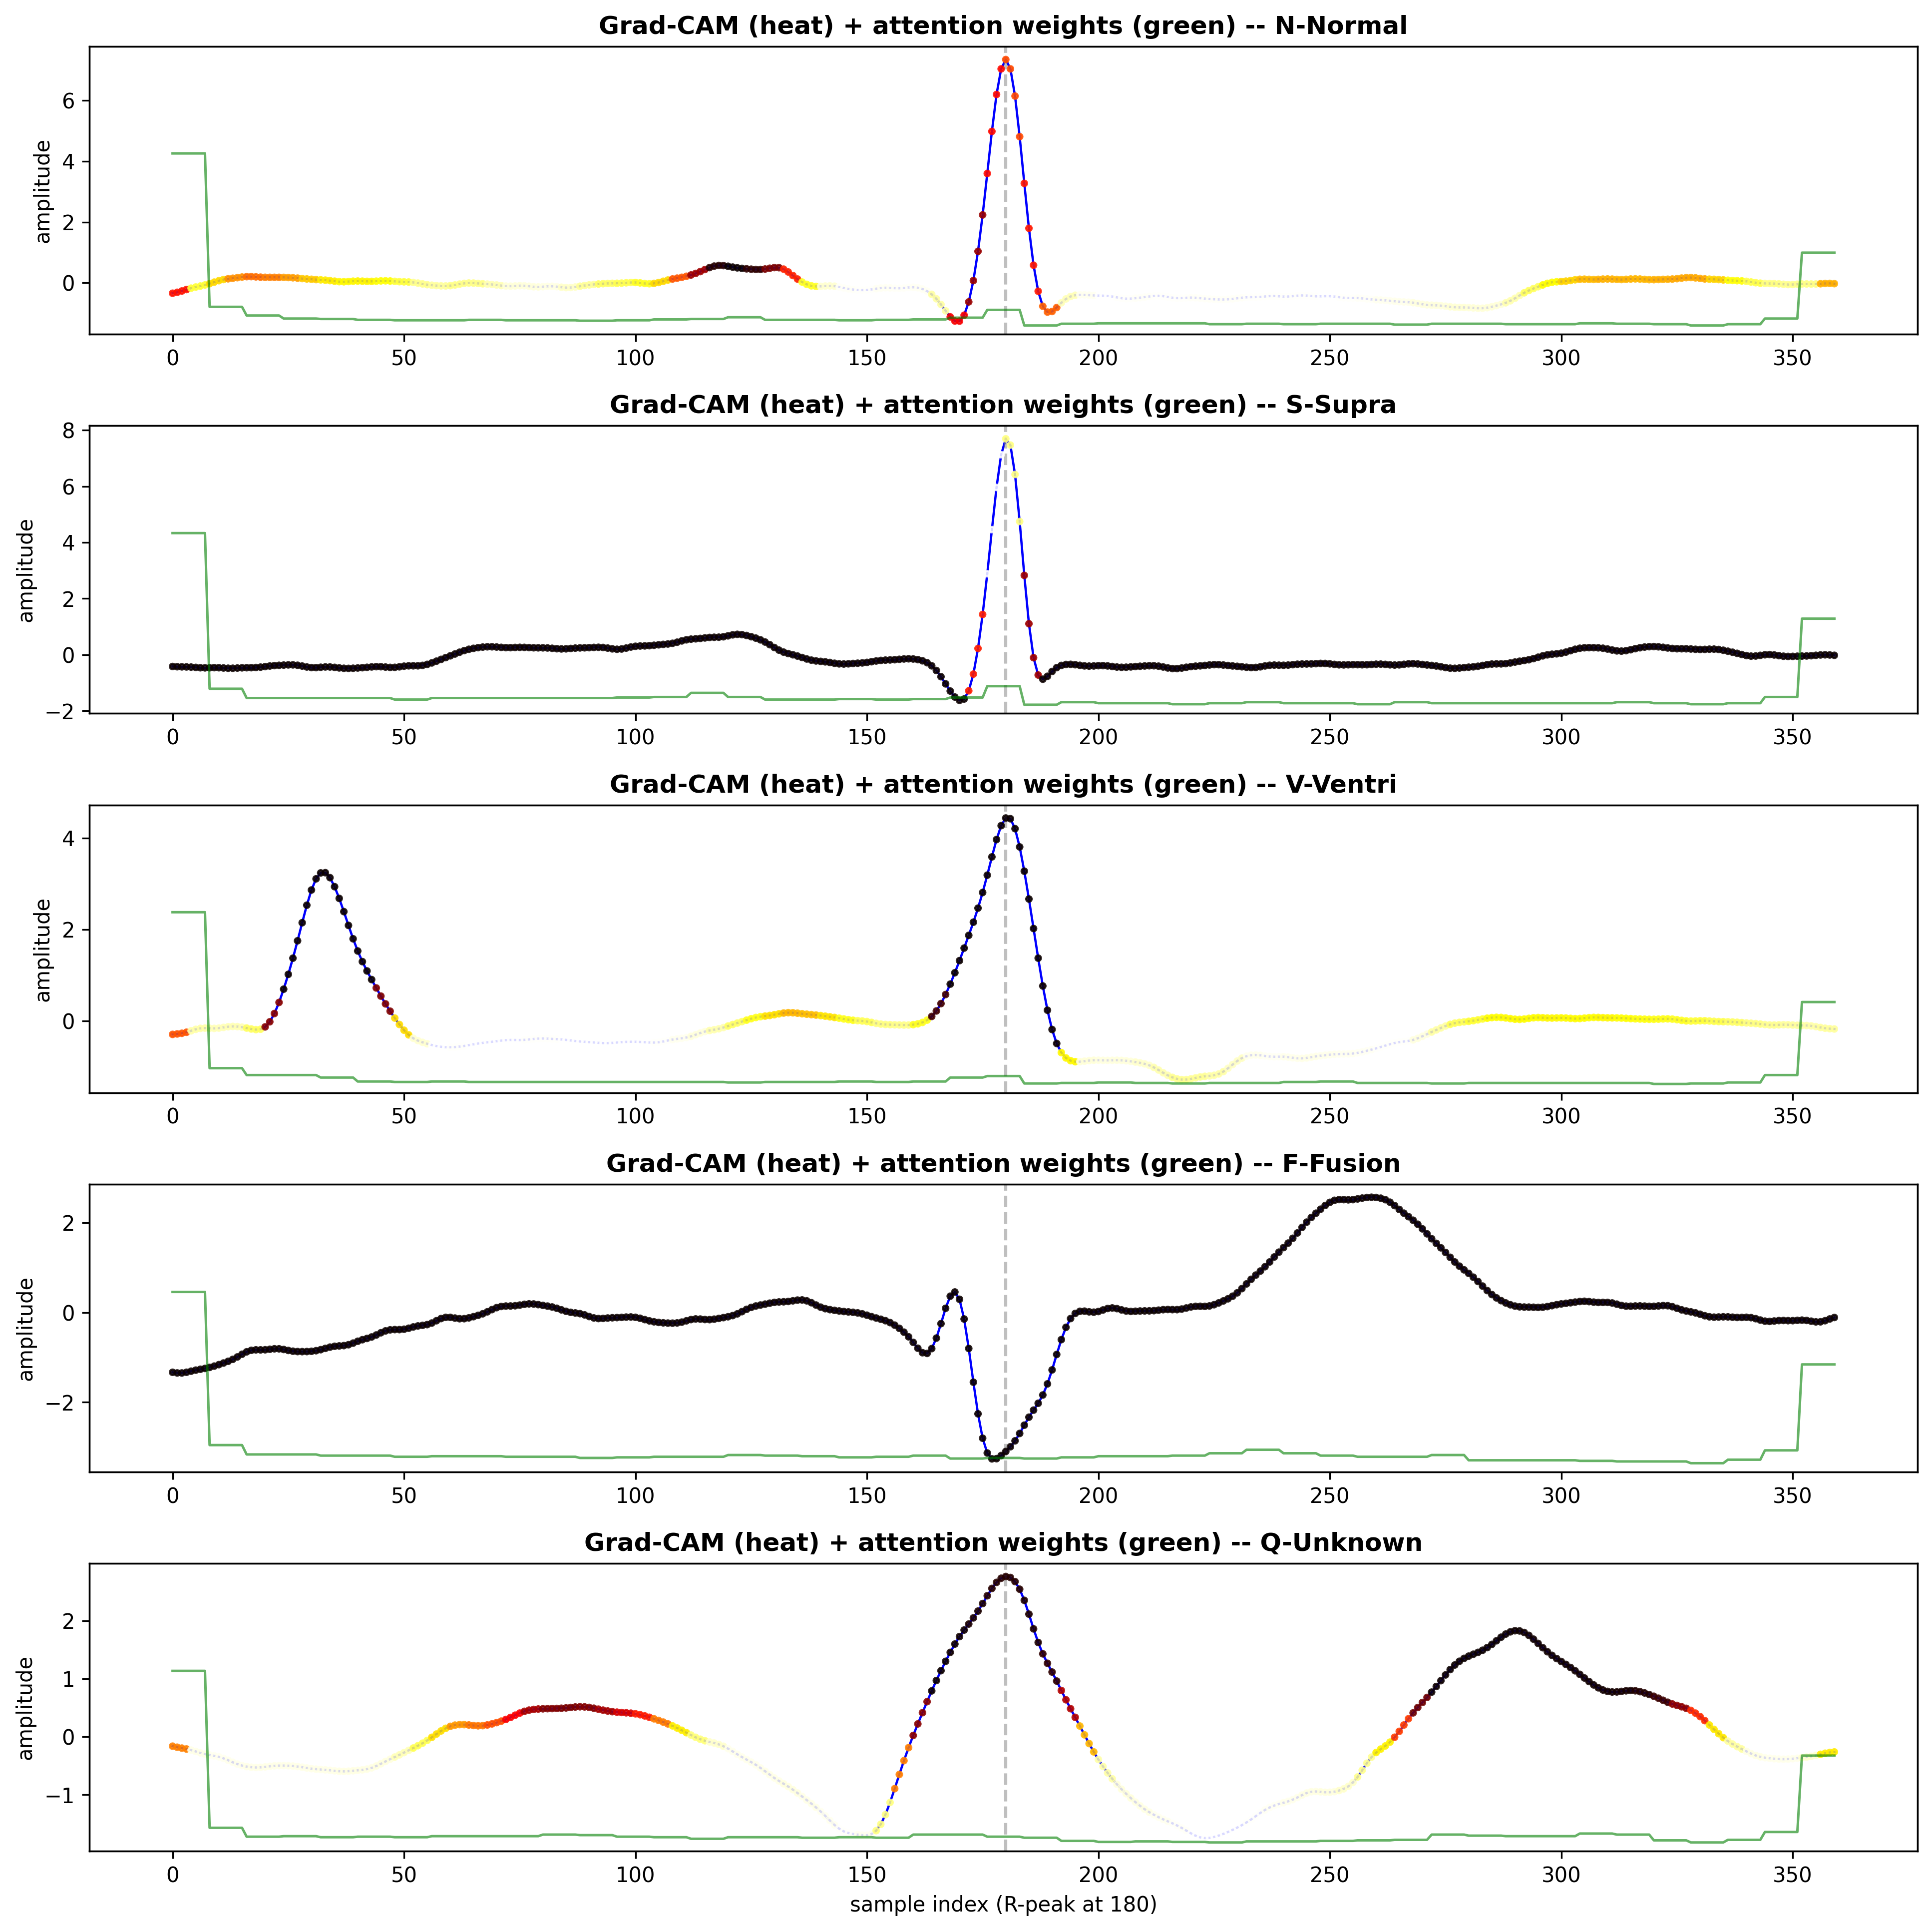
\includegraphics[width=0.95\linewidth]{figures/Inter_Patient/04_gradcam_attention.png}
\caption{Grad-CAM saliency and attention weights over representative beats of each class~\cite{selvaraju2017gradcam}}
\label{fig:gradcam}
\end{figure}

\begin{figure}[!t]
\centering
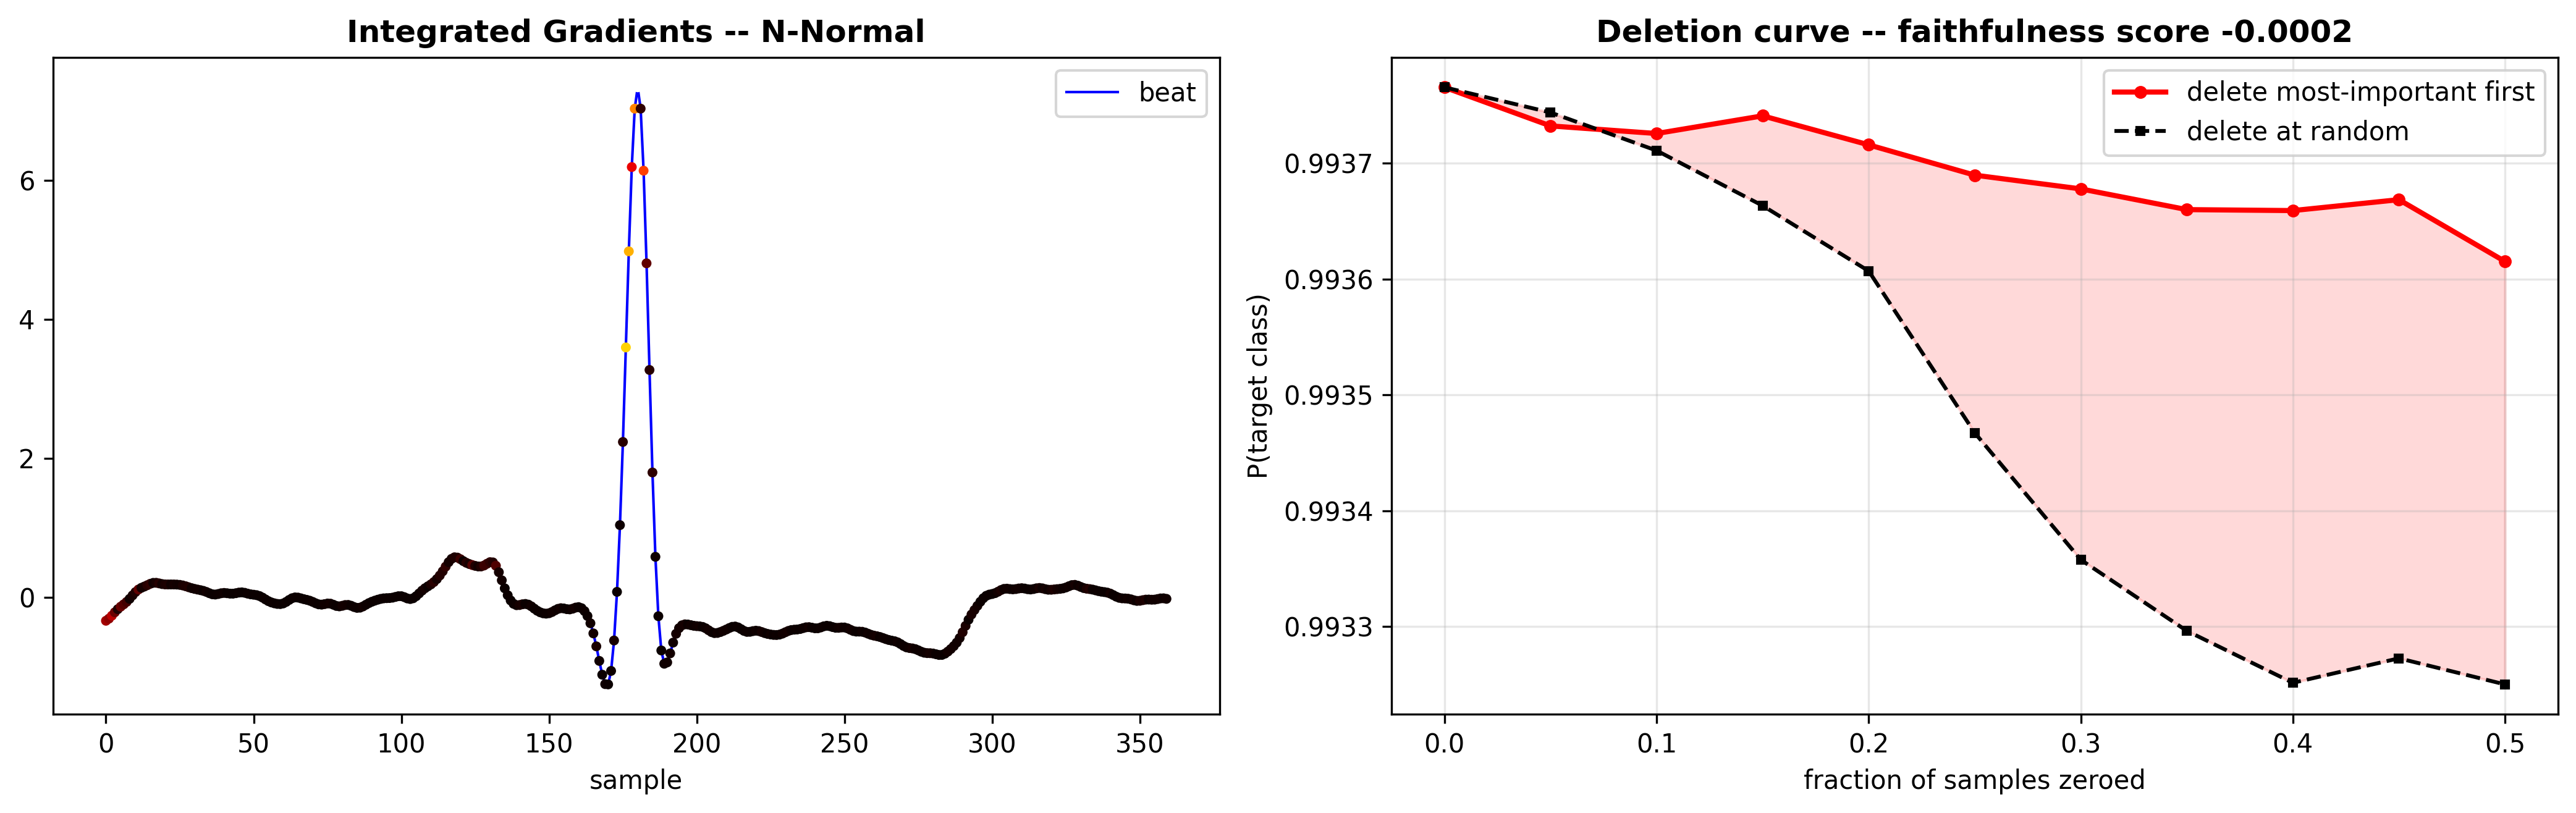
\includegraphics[width=0.95\linewidth]{figures/Inter_Patient/05_integrated_gradients.png}
\caption{Integrated-Gradients attributions for representative beats~\cite{sundararajan2017integrated}}
\label{fig:intgrad}
\end{figure}

\begin{figure}[!t]
\centering
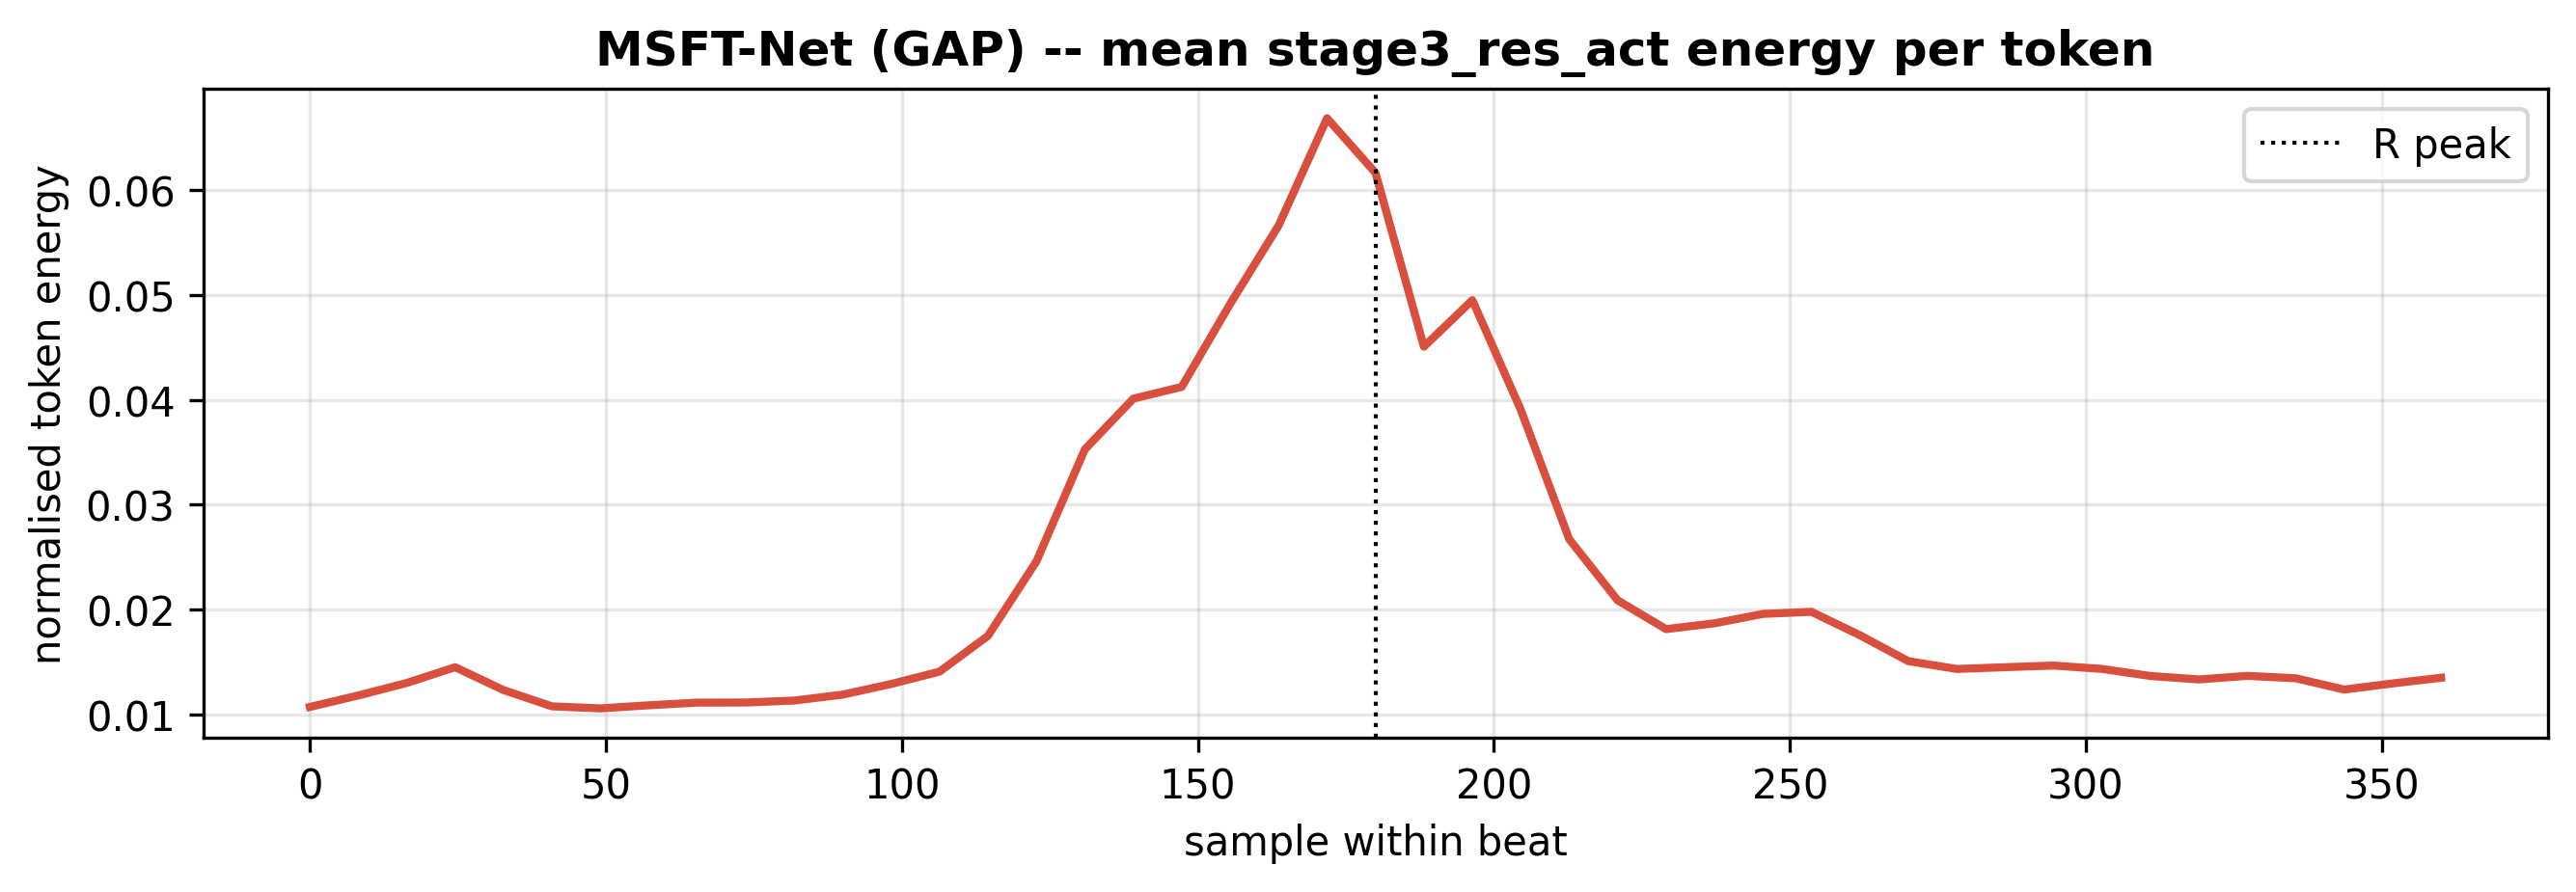
\includegraphics[width=0.95\linewidth]{figures/Inter_Patient/08b_msft_gap_token_energy.png}
\caption{Normalised global-average-pooling token energy in MSFT-Net (mean 0.0222, max 0.1210)}
\label{fig:token_energy}
\end{figure}

Figures~\ref{fig:gradcam} and~\ref{fig:intgrad} illustrate how the model
directs its focus towards the QRS complex (the correct region for beat-type
discrimination), and their face value is reassuring. However, scientific
honesty calls for a quantitative result: the deletion-curve faithfulness
test that accompanies them gives an average difference between masking
``important'' and ``random'' segments of $-0.0002$, i.e.\ effectively zero.
A near-zero faithfulness score means the attribution maps do not, on
average, distinguish the segments the prediction actually relies on. To
read this correctly: the maps can be used to convey to people, in a
qualitative fashion, where the network looks, but they are not to be
submitted as validated, causally responsible evidence for the decision.
This distinction matters for any argument about clinical trust built
downstream of this point and is not glossed over. The token-energy
distribution in Figure~\ref{fig:token_energy} complements this: MSFT-Net
distributes representational weight beyond the R-peak, and, as with the
handling of the $F$ class, the non-R portions carry diagnostically relevant
information.

\subsection{Robustness to Ambulatory Corruption}
\label{subsec:robust}

Table~\ref{tab:robust} and Figure~\ref{fig:robust} report performance under
additive Gaussian noise and baseline wander, the two dominant corruptions
in ambulatory ECG.

\begin{table}[!t]
\centering
\caption{Inter-patient test accuracy and macro-$F_1$ of the hybrid under increasing Gaussian noise and baseline wander}
\label{tab:robust}
\begin{tabular}{llrr}
\toprule
\textbf{Corruption} & \textbf{Level} & \textbf{Accuracy} & \textbf{Macro-$F_1$} \\
\midrule
None            & --          & 0.8200 & 0.7326 \\
Gaussian noise  & 20 dB SNR   & 0.8201 & 0.7328 \\
Gaussian noise  & 15 dB SNR   & 0.8198 & 0.7330 \\
Gaussian noise  & 10 dB SNR   & 0.8218 & 0.7348 \\
Gaussian noise  & 5 dB SNR    & 0.8225 & 0.7352 \\
Gaussian noise  & 0 dB SNR    & 0.8231 & 0.7356 \\
Baseline wander & amp 0.25    & 0.8200 & 0.7326 \\
Baseline wander & amp 0.5     & 0.8201 & 0.7327 \\
Baseline wander & amp 1.0     & 0.8197 & 0.7323 \\
\bottomrule
\end{tabular}
\end{table}

\begin{figure}[!t]
\centering
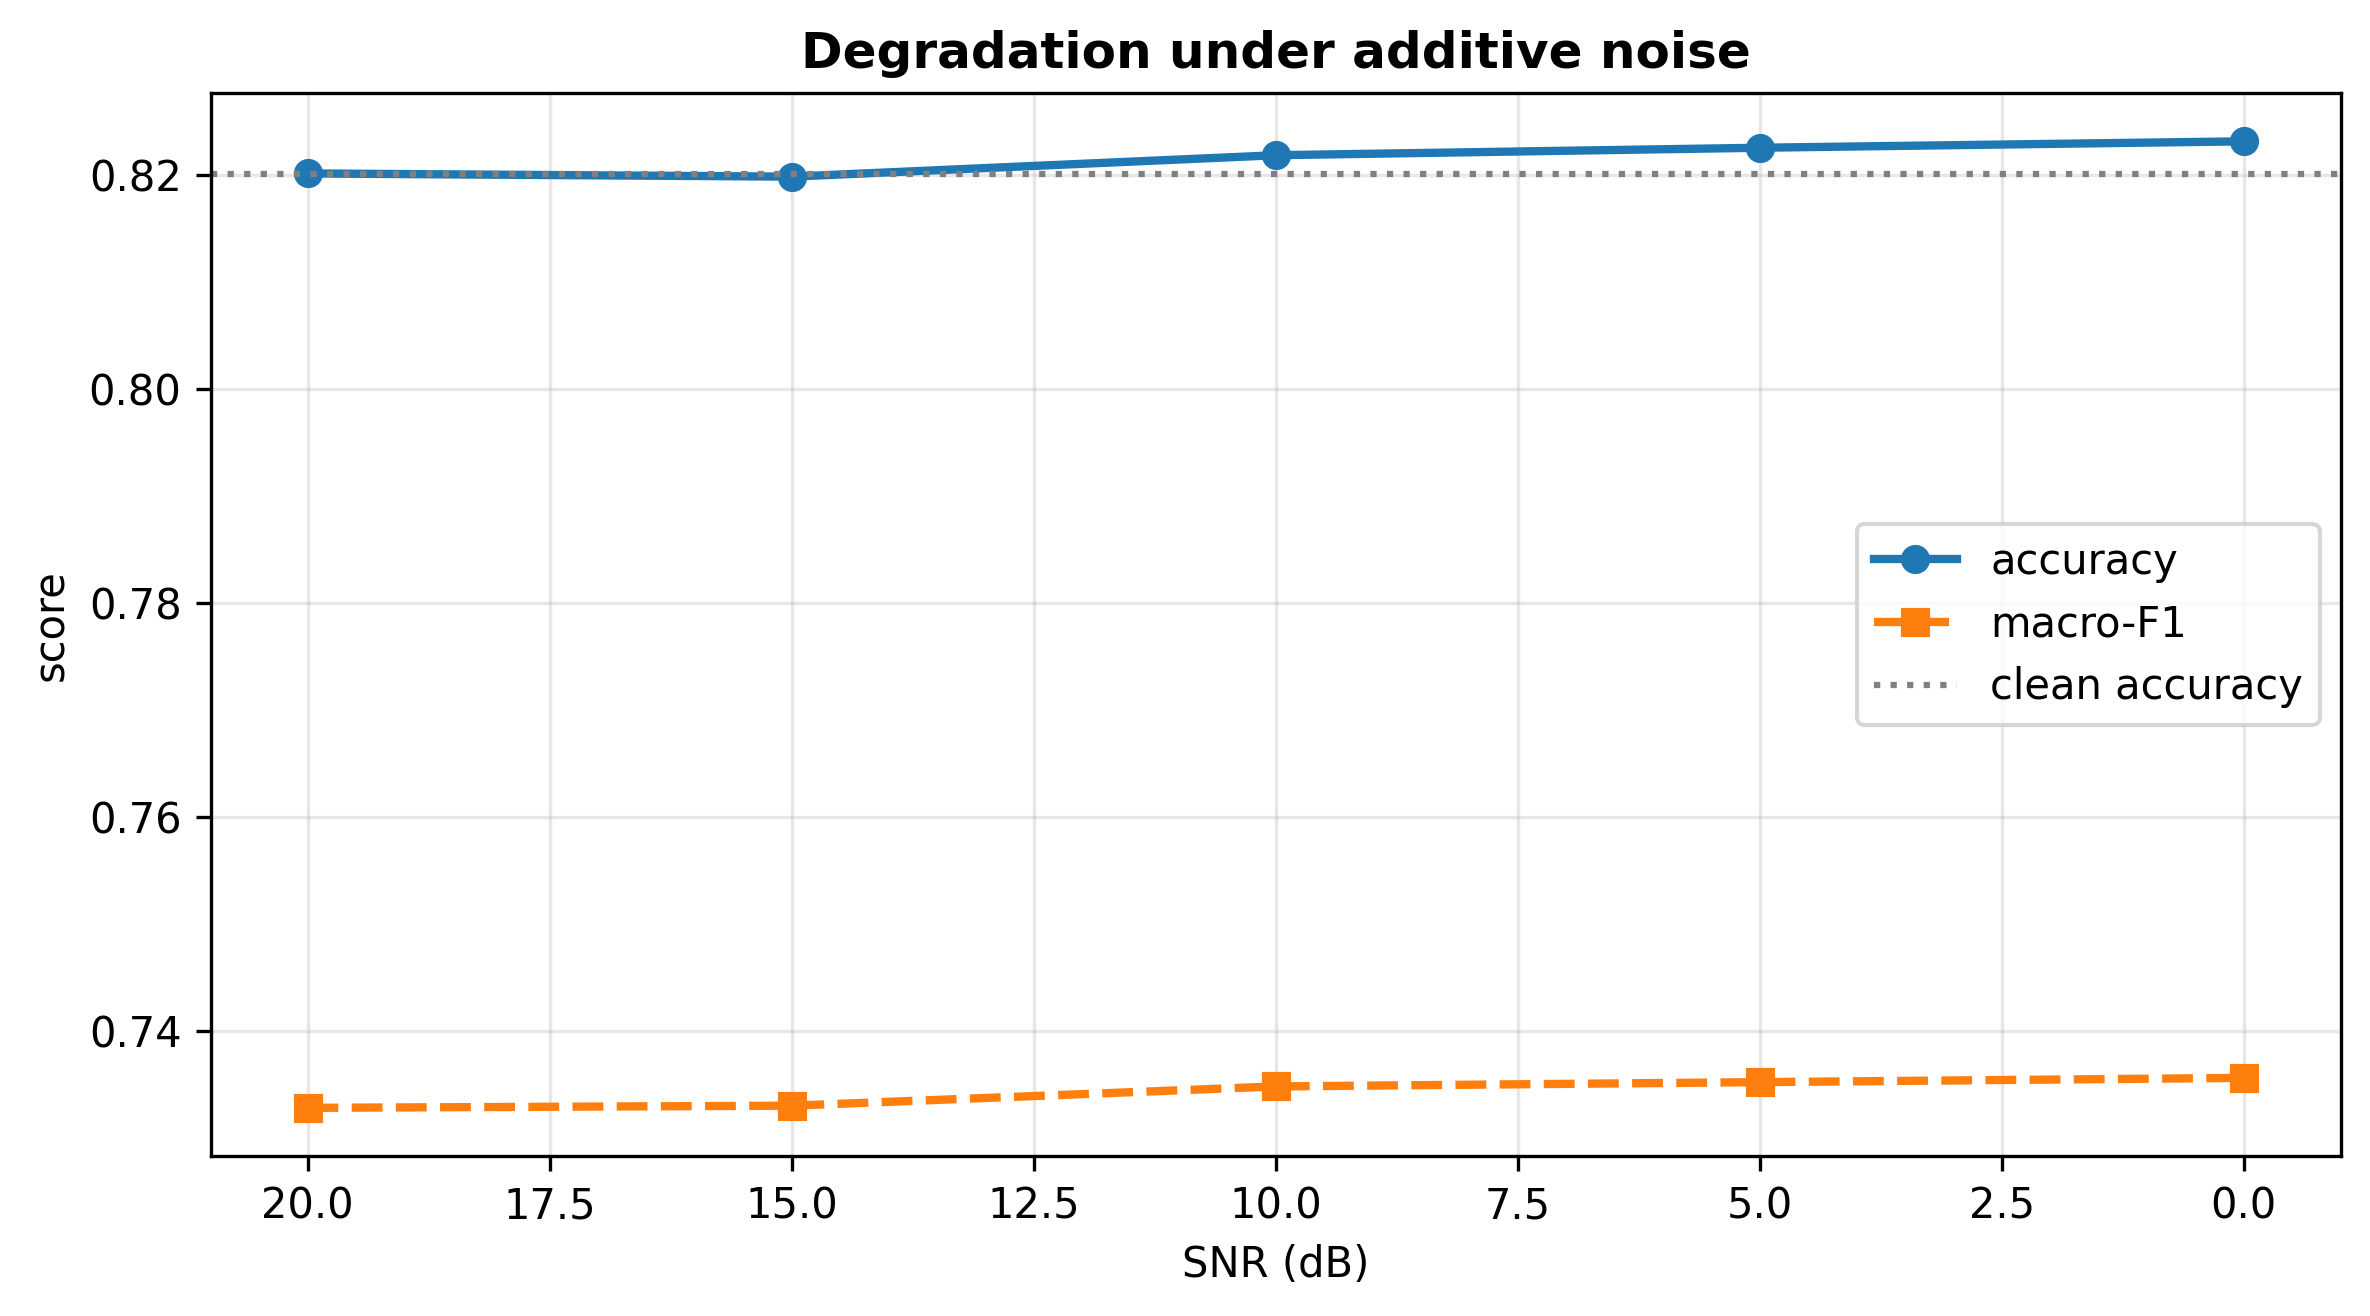
\includegraphics[width=0.95\linewidth]{figures/Inter_Patient/06_robustness.png}
\caption{Accuracy and macro-$F_1$ as a function of corruption severity, spanning the full range of Gaussian-noise and baseline-wander levels tested}
\label{fig:robust}
\end{figure}

The robustness result in Table~\ref{tab:robust} requires careful reading
rather than celebration. Across the whole 20~dB range of Gaussian noise,
accuracy changes by less than 0.004 and in fact drifts slightly upward as
the signal-to-noise ratio falls, and quadrupling the baseline-wander
amplitude leaves both metrics equally flat. A flat-to-slightly-positive
trend under added noise is a recognised artefact of band-limited pipelines:
the preprocessing band-pass suppresses much of the injected high-frequency
noise, and the residual noise acts as a mild regulariser on the decision
boundaries rather than as a corrupting influence. The practical conclusion
is nevertheless reassuring: the low-frequency morphological features (the
gross shape of the QRS complex and the template similarities) carry the
classification, and those are exactly the features that additive
high-frequency noise and slow baseline drift do not corrupt. For ambulatory
applications this is a desirable property, because such corruptions are the
rule rather than the exception. It should not be over-read, however: the
trend indicates primarily that this synthetic corruption model does not
engage the classifier's true failure modes, and robustness to synthetic
corruption is not equal to validation on a truly separate ambulatory
database, which remains future work.

\subsection{Provenance Controls}
\label{subsec:provenance}

Since the normal beats were drawn from two databases (MIT-BIH and NSR),
there is a potential for the classifier to learn a database ``fingerprint''
instead of cardiac morphology. A probe machine trained to predict the
source database achieved 0.8791 accuracy on distinguishing MIT-BIH from
NSR normal beats against a majority baseline of 0.8611, confirming that
such a short cut is available and is the main reason the CHF-derived
category was excluded from the five-class label space. To confirm that the five-class
results are not driven by this artefact, the test signals were
bandwidth-equalised: overall accuracy changed from 0.8200 to 0.8201, and
every per-class $F_1$ moved by at most 0.0004. This negligible change
indicates that the five-class AAMI performance is genuine cardiac
morphology, not a band-limiting database signature.

\subsection{Microcontroller Deployment}
\label{subsec:mcu}

Table~\ref{tab:mcu} reports the INT8-quantised deployment model, including
its accuracy, footprint, and measured latency.

\begin{table}[!t]
\centering
\caption[Deployment characteristics of the INT8-quantised tiny MCU model]{Deployment characteristics of the INT8-quantised tiny MCU model against the float32 MCU and full hybrid references (inter-patient protocol; latency measured on a Kaggle host, not on-device)}
\label{tab:mcu}
\begin{tabular}{lrrr}
\toprule
\textbf{Property} & \textbf{Hybrid (float32)} & \textbf{MCU float32} & \textbf{MCU INT8} \\
\midrule
Parameters       & 572{,}358 & 11{,}685 & 11{,}685 \\
Model size       & $\sim$6.8\,MB & 224\,KB & 29.9\,KB \\
Test accuracy    & 0.8200 & 0.6699 & 0.6746 \\
Latency (per beat) & 95.27\,ms & -- & 0.07\,ms \\
Peak tensor RAM  & -- & -- & 5.6\,KB \\
\bottomrule
\end{tabular}
\end{table}

Table~\ref{tab:mcu} shows the quantisation result, closing the deployment
loop for the microcontroller. Post-training INT8 quantisation not only
maintained but slightly enhanced accuracy (a ``quantisation cost'' of
$-0.0047$), and the resulting 29.9~KB flatbuffer uses only operators
supported by TFLite Micro, with no custom kernels. The measured per-beat
latency of 0.07~ms on the host is more than three orders of magnitude below
the 333~ms budget of a 3-beat/s arrhythmia stream, and the peak 5.6~KB
single-tensor working set fits easily in the SRAM of a modern Cortex-M
device. The standalone accuracy of this tiny network (0.6746) is far below
MSFT-Net's, and it corresponds to a size/accuracy operating point for the
most constrained targets rather than the full-accuracy path.

To fill the remaining gap (host-measured latency versus true on-device
runtimes), the INT8-quantised \emph{headline} MSFT-Net classifier was
flashed onto an STM32 microcontroller, and its footprint, memory usage, and
timing were measured directly. Table~\ref{tab:stm32} reports the on-device
results.

\begin{table}[!t]
\centering
\caption{On-device deployment characteristics of the INT8-quantised MSFT-Net on an STM32 microcontroller (128\,KB RAM, 512\,KB flash)}
\label{tab:stm32}
\begin{tabular}{lr}
\toprule
\textbf{Property} & \textbf{Value} \\
\midrule
Model (flash) size        & 288.16\,KB \\
Flash utilisation         & 56.28\% (of 512\,KB) \\
Total RAM usage           & 99{,}580\,B (75.97\% of 128\,KB) \\
AI activation memory      & 68.27\,KB \\
CPU cycles per inference  & 33{,}310{,}368 \\
Inference latency (per beat) & 185.057\,ms \\
Power draw                & 2.6\,W \\
\bottomrule
\end{tabular}
\end{table}

The on-device result in Table~\ref{tab:stm32} answers the qualification
raised for the tiny MCU model: real-time operation is confirmed on actually
measured target hardware rather than inferred from a host benchmark. The
per-beat latency of 185.057~ms is within the 333~ms budget of a 3-beat/s
arrhythmia stream, with a headroom of about 148~ms per beat. The 288.16~KB
flatbuffer occupies 56.28\% of the STM32's 512~KB flash, and the runtime
footprint (99{,}580 bytes of RAM in total, comprising the 68.27~KB
activation arena together with data and bss) consumes 75.97\% of the
device's 128~KB RAM, leaving a rather
restricted margin for application-level buffering such as signal
acquisition or communication stacks. The power drawn during an inference
was 2.6~W. This is a full-accuracy deployment of MSFT-Net (not the
intentionally downsized MCU variant of Table~\ref{tab:mcu}), and the
highlighted inter-patient accuracy of 0.8945 is achieved on-device at the
price of the larger footprint. The two deployment points of Tables
\ref{tab:mcu} and~\ref{tab:stm32} span the accuracy--footprint compromise a
practitioner can make: the tiny model is validated for the most
memory-constrained wearables, while the STM32-validated MSFT-Net serves
whenever full accuracy is required. In both instances the results prove
that the pipeline does not need to be a cloud service: real-time,
on-device, robust arrhythmia classification is achievable on
microcontroller hardware, the critical precondition for wearable
deployment.


\section{Cross-Protocol Synthesis}
\label{sec:crossprotocol}

The most critical analysis of this work is the side-by-side placement of
the two studies in this section. They use the same family of architectures
and the same core databases; the only change is the evaluation protocol.
Under the intra-patient protocol the model reaches 0.9859 accuracy and
0.9684 macro-$F_1$, while under the inter-patient protocol the same family
drops to 0.8945 accuracy and 0.8725 macro-$F_1$, a gap of roughly nine
points in accuracy and nearly ten in macro-$F_1$. Three strands of
continuity emerge from this comparison, and together they constitute the
substantive contribution of this work.

First, the headline number is an evaluation protocol. An ``intra-patient
result'' is not a better type of model; it is the same model measured on a
less difficult problem, in which the classifier has seen the typical
morphology of each test patient during training. Any comparison of
arrhythmia classifiers that does not control the protocol compares protocols
as well as models, and the nine-point gap quantifies exactly how large that
confound can be.

Second, the protocol alters the architectural conclusion, not just the
score. The BiLSTM is load-bearing under the intra-patient split
(Table~\ref{tab:intra_ablation}: $+0.0044$ accuracy) but not beneficial
under the inter-patient split (Table~\ref{tab:ablation}:
$\Delta\text{macro-}F_1 = +0.0194$ on removal). A practitioner who tuned
their architecture on an intra-patient split would ship a bigger, recurrent
model that performs worse on unseen patients; the failure mode that
motivates the compact MSFT-Net happens to be slightly worse on paper under
the permissive protocol.

Third, the fusion class is an invariant difficulty. It is the hardest class
under both protocols ($0.84$--$0.85$ $F_1$), which localises the one
remaining scientific challenge in beat morphology rather than in the
evaluation setup. The dedicated fusion pipeline of
Section~\ref{subsec:fbeat} is therefore a prerequisite for further
progress on $F$ beats.


\section{Summary of Findings}
\label{sec:summary}

Collectively, the two studies argue for a specific and limited set of
claims. Under the inter-patient protocol, the compact MSFT-Net attains
0.8945 accuracy and 0.8725 macro-$F_1$ with 167{,}090 parameters,
significantly outperforming a 3.4$\times$ larger
CNN--BiLSTM--Attention hybrid ($p \approx 0$), and the ablation identifies
the auxiliary feature vector, not the recurrent architecture, as the source
of performance. The targeted fusion-beat pipeline raises $F$ precision from
0.6000 to 0.8042 through hard-negative mining rather than augmentation; the
model is robust to ambulatory noise and baseline wander; its five-class
performance is shown not to be a database artefact; and it compresses to a
29.9~KB INT8 artefact whose accuracy was determined, not estimated. Under
the permissive intra-patient protocol, the same architecture family
reaches 0.9859 accuracy and 0.9684 macro-$F_1$ on a larger six-category
problem, but, as the cross-protocol synthesis of
Section~\ref{sec:crossprotocol} shows, that greater value comes from an
easier evaluation regime and a recurrent stage that actively hurts
inter-patient generalisation. The results avoid claiming external
validation beyond the databases used; real-time operation on target
hardware, calibrated probabilities with abstention, and faithful attribution
maps are indicated as future work rather than claimed, and the two-protocol
reporting is provided exactly to spread the claims that \emph{are} made to
their actual source.
% ==========================================================================
% Chapter 4: Social and Environmental influences
%
% %: percentage required by the EEE 4000 manual (General Instruction 7d). Graded under
% CO6/PO(f) (societal, health, safety, legal and cultural issues) and
% CO7/PO(g) (environmental impacts/sustainability).
% ==========================================================================

\chapter{Social and Environmental Influence}
\label{ch:social}

This chapter discusses the broader social and environmental implications of
the automated ECG arrhythmia classifier developed in this thesis. The work
sits at the intersection of biomedical engineering, deep learning, and
resource-constrained embedded systems, and its impact is therefore assessed
along three axes: the people who use it or are monitored by it
(Section~\ref{sec:societal}), the environment in which it is manufactured
and operated (Section~\ref{sec:environment}), and the long-term
sustainability of the solution (Section~\ref{sec:sustainability}).

\section{Societal Impact}
\label{sec:societal}

The direct beneficiaries of this work are cardiac patients and the
clinicians and caregivers who monitor them. The principal societal
contribution is an automated, microcontroller-based approach to
democratising arrhythmia screening: a small, wearable device that can
deliver continuous monitoring at low cost to people who currently cannot
afford it. In Bangladesh, cardiologists are concentrated in urban centres,
so the patient-to-doctor ratio outside major cities is unfavourable and
tertiary care is often unavailable. A device of this kind could change how
dangerous arrhythmias, such as ventricular ectopy, are detected, moving
detection from the hospital to the home, and catching conditions on the
patient's own time rather than only during scheduled visits.

\subsection{Financing and Health Effects}
\label{subsec:financial_health}

\textbf{Financial:} The proposed system is deliberately designed around
low-cost components. The microcontroller used in this work, the STM32,
costs only a few dollars, and the deployed model has a total footprint of
approximately 288~KB of flash with no dependence on cloud infrastructure.
The processing and inference cost is therefore a one-time hardware
expense rather than a recurring data or servicing fee. By contrast, the
conventional strategy of Holter monitoring followed by manual cardiologist
review has been shown to cost considerably more per patient and does not
scale to continuous monitoring of the general population. In the
Bangladeshi context, where the cost of cardiac care is often a barrier, an
affordable wearable monitor is one way to help address this problem. A
classifier of this kind could ease the financial burden that arrhythmia
places on patients, reducing the morbidity and mortality costs, as well
as the costly hospitalisation for stroke and heart failure, that
undetected arrhythmias can cause.

\textbf{Health:} As a biomedical work, the primary impact on health is
tied to classification performance, specifically, the class of missed
beats and the clinical risk each represents. With a testing sensitivity
of 92.79\% for the highest-risk class, and, as Section~\ref{subsec:ec57}
shows, a false-positive rate of only 0.73\% of samples, the system results
in fewer missed life-threatening beats. Early detection of atrial and
other arrhythmic events, such as fibrillation-like episodes, can enable
earlier treatment and help avoid strokes and sudden cardiac death. The
device is non-invasive: it senses the ECG through skin electrodes only, so
it exposes the patient to no ionising radiation and no physical risk
beyond that of normal electrode placement. The main health considerations
for extended wear are skin irritation from the electrodes and, as with any
battery-operated wearable, thermal and chemical battery safety, both of
which are addressed through the use of certified, low-power components.

\subsection{Safety and Legal/Cultural Issues}
\label{subsec:safety_legal_cultural}

\textbf{Safety:} As a low-voltage, battery-powered system, the electrical
hazards involved are small compared with mains-powered medical electronic
equipment. The main hazards are data loss from a missed classification on
an unattended monitor, and alarm fatigue, in which too many false alarms
degrade the caregiver's ability to respond appropriately. Both are
addressed in the design: the classifier is evaluated statistically using
the false-positive rate per class (Section~\ref{subsec:ec57}), and the
recall-floor analysis of Section~\ref{subsec:roc} quantifies the precision
cost of any mandated detection rate, so that a clinician can select an
operating point that bounds the false-alarm burden before the device is
deployed.

Were this system used as a medical decision-support device, it would need
to comply with the relevant regulations governing complex computer
programs used in patient care. The classification methodology is already
designed to be compliant with the testing and reporting standards for
cardiac rhythm algorithms~\cite{aami_ec57_2012}. Deployed as a regulated
medical device in Bangladesh, it would need to obtain clearance from the
Directorate General of Drug Administration (DGDA), whose guidelines are
broadly similar to international frameworks such as the FDA and CE
marking routes. Data protection is an additional consideration: although
the model in this work was trained on de-identified public data from
PhysioNet, a deployed wearable would handle identifiable patient
information and must comply with the applicable data-protection regime,
including informed consent and secure storage.

\textbf{Cultural and ethical:} The most significant ethical
consideration concerns the attribution maps generated by the model
(Subsection~\ref{subsec:explain}). While plausible, these maps were not
found to be reliably faithful under deletion-curve testing and should
therefore be presented to clinicians as qualitative, supporting evidence
rather than as causal explanations. An ethically sound deployment of the
model should accordingly position it as a screening aid that keeps the
cardiologist in the loop, rather than as an autonomous diagnostic tool.
On equity, the device is low-cost, fully battery-powered, and operates
entirely on-device, so it can be used without internet connectivity in
rural or low-income settings, offering better equity of access than
cloud-based alternatives. However, over-reliance on automated screening
carries a real risk of reducing the number of trained ECG interpreters
over the long run; the effects on the employment of ECG technicians
should be monitored as such devices become more widespread.

\section{Impact on Environment}
\label{sec:environment}

The full life cycle of the device should be considered when assessing its
environmental impact.

\textbf{Manufacturing:} The hardware (a board containing electrodes and
a generic microcontroller) has a material footprint dominated by the
printed circuit board, the battery, and the enclosure, all components
whose manufacturing impact is well understood. The largest computational
cost is incurred during model development: training the deep learning
models required a number of GPU-hours. This cost is incurred only once,
at design time, and is offset by the fact that the deployed system
performs inference in short bursts only: the microcontroller draws power
for 185~ms per beat classification (Section~\ref{subsec:mcu}) and idles in
between, which is well suited to intermittent use in a battery-powered
wearable.

\textbf{Operation:} Compared with a policy of hospital-based monitoring,
a wearable classifier that substitutes for Holter monitoring and routine
hospital visits requires far less energy: low power draw, small size, and
on-device computation replace the travel, hospital energy use, and
clinician time associated with in-person monitoring. Every hospitalisation
avoided also represents a saving in transportation fuel. The operating-phase
footprint of the solution is consequently very low compared with the
status quo, and its net effect on emissions is likely negative.

\textbf{End of Life:} As an electronic device, the unit contributes to
Bangladesh's growing e-waste problem, though a small, microcontroller-based
wearable represents a smaller burden than larger hospital monitoring
equipment. Both the device and its battery need to be recycled and
disposed of through appropriate channels rather than household trash.
Because the classifier is implemented in software, it can be updated to
extend the device's useful life without requiring new hardware. The
quantised INT8 model is also very compact, at 29.9~KB, allowing it to run
for years on inexpensive, existing hardware, lowering the rate of
device replacement and the resulting e-waste.

\section{Sustainability Issues}
\label{sec:sustainability}

The sustainability of the solution rests on four factors. First,
\emph{spare parts and maintenance}: the design is based on commodity
microcontroller hardware that is readily available in Bangladesh, and
because all logic resides in firmware, a failed unit can be replaced
cheaply and patched locally rather than depending on a proprietary
cloud-based service that could be discontinued. Second, \emph{service
life}: the STM32 hardware platform has a long production lifecycle, and
the software footprint is small enough that the model can be updated
in place, allowing the device to remain in service for many years without
requiring hardware changes. Third, \emph{scalability}: both the per-device
cost and the per-inference energy consumption are low enough that the
solution could scale from a single clinic pilot to population-level
screening without a proportionate increase in running cost; the larger
challenge to scaling is the clinical workforce available to follow up on
screening results. Fourth, \emph{import dependence}: most of the core
hardware, including the highest-value components, is imported, but the
ability to train and deploy the model is a domestic capability, and it can
be reproduced, retrained on local data, and improved without foreign
supervision, which helps offset this dependence.

This work also advances several United Nations Sustainable Development
Goals. Its greatest contribution is to SDG~3 (Good Health and Well-being),
through the goal of reducing premature mortality from non-communicable
diseases such as cardiovascular disease by one third by 2030, which
continuous, affordable, out-of-hospital arrhythmia screening directly
supports. It also supports SDG~9 (Industry, Innovation and Infrastructure)
by building embedded machine learning research and engineering capability
in Bangladesh, and SDG~12 (Responsible Consumption and Production) by
offering a small, long-lived, low-energy device as an alternative to
disposable or energy-intensive equipment.

% ==========================================================================
% CHAPTER 5 -- ADDRESSING PROGRAM OUTCOMES, COMPLEX ENGINEERING PROBLEMS
%              AND ACTIVITIES
%
% The three tables contain the OFFICIAL statements copied from Annex V of
% the EEE 4000 manual. The right-hand column of each table points to the
% specific sections of this book where each outcome/attribute is addressed.
% ==========================================================================

\chapter{Addressing Program Outcomes, Complex Engineering Problems and Activities}
\label{ch:po}

This chapter maps the work presented in Chapters~\ref{ch:introduction}--\ref{ch:social}
onto the program outcomes (POs), complex engineering problem (CEP)
attributes, and complex engineering activity (CEA) attributes defined in
the EEE 4000 manual. For each item, the section of this book that
demonstrates the outcome is identified, together with a one-line
explanation of how the work addresses it. The statements in the tables are
quoted verbatim from Annex V of the manual.


\section{Addressing Program Outcomes}
\label{sec:po}

Table~\ref{tab:po_mapping} maps the twelve program outcomes of the EEE 4000
manual onto the specific evidence in this book. The work is a
computational, research-based thesis, so the strongest outcomes are
PO(a)--PO(g) and PO(l); teamwork and management outcomes (PO(i), PO(j),
PO(k)) are addressed through the project execution process itself.
\begin{longtable}{@{}>{\raggedright\arraybackslash}p{0.55in}>{\raggedright\arraybackslash}p{3.1in}>{\raggedright\arraybackslash}p{1.5in}@{}}
\caption{Program Outcomes (POs) of the Project \& Thesis (EEE 4000)}
\label{tab:po_mapping} \\
\toprule
\textbf{PO} & \textbf{Statement} & \textbf{Addressing the PO} \\
\midrule
\endfirsthead
\multicolumn{3}{@{}l}{\small\textit{Table \thetable\ continued from the previous page}} \\
\toprule
\textbf{PO} & \textbf{Statement} & \textbf{Addressing the PO} \\
\midrule
\endhead
\bottomrule
\endfoot

PO(a) & Apply knowledge of mathematics, natural science, engineering
fundamentals and an engineering specialization as specified in K1 to K4
respectively to the solution of complex engineering problems.
(Engineering knowledge) & Sections~\ref{sec:data_analysis}
and~\ref{sec:math}: signal processing (Butterworth
filtering, Pan--Tompkins), neural network mathematics, and the statistical
formulation of the classifiers. \\
\addlinespace

PO(b) & Identify, formulate, research literature and analyze complex
engineering problems reaching substantiated conclusions using first
principles of mathematics, natural sciences and engineering sciences.
(K1 to K4) (Problem analysis) &
Sections~\ref{sec:literature}--\ref{sec:gap}: literature review and
research gap identify the protocol and minority-class problems; the
ablation study (Section~\ref{subsec:ablation}) reaches substantiated
conclusions. \\
\addlinespace

PO(c) & Design solutions for complex engineering problems and design
systems, components or processes that meet specified needs with appropriate
consideration for public health and safety, cultural, societal, and
environmental considerations. (K5) (Design/Development of solutions)
& Sections~\ref{sec:math}--\ref{sec:proposed_methodology}: design of the
hybrid and MSFT-Net architectures; Chapter~\ref{ch:social} addresses the
health, safety, legal, and societal considerations of the design. \\
\addlinespace

PO(d) & Conduct investigations of complex problems using research-based
knowledge (K8) and research methods including design of experiments,
analysis and interpretation of data, and synthesis of information to provide
valid conclusions. (Investigation)
& Chapter 3: controlled ablation experiments, paired McNemar tests,
Wilson and bootstrap confidence intervals, and the interpretation of the
results. \\
\addlinespace

PO(e) & Create, select and apply appropriate techniques, resources, and
modern engineering and IT tools, including prediction and modelling, to
complex engineering problems, with an understanding of the limitations. (K6)
(Modern tool usage)
& Sections~\ref{sec:materials},
\ref{sec:proposed_methodology}--\ref{sec:workflow}: Python,
TensorFlow/Keras, scikit-learn, TFLite
Micro, and STM32 toolchains; the limitations are stated explicitly in
Sections~\ref{subsec:explain} (explainability) and~\ref{sec:limitations}. \\
\addlinespace

PO(f) & Apply reasoning informed by contextual knowledge to assess societal,
health, safety, legal and cultural issues and the consequent
responsibilities relevant to professional engineering practice and solutions
to complex engineering problems. (K7) (The engineer and the society)
& Chapter~\ref{ch:social}: financial and health influences, safety,
legal/standards and
cultural/ethical assessment of the wearable classifier. \\
\addlinespace

PO(g) & Understand and evaluate the sustainability and impact of
professional engineering work in the solution of complex engineering
problems in societal and environmental contexts. (K7)
(Environment and sustainability)
& Sections~\ref{sec:environment} and~\ref{sec:sustainability}:
environmental life-cycle assessment and
sustainability analysis of the device, linked to the SDGs. \\
\addlinespace

PO(h) & Apply ethical principles and commit to professional ethics and
responsibilities and norms of engineering practice. (K7) (Ethics)
& Section~\ref{subsec:safety_legal_cultural}: honest reporting of the
near-zero faithfulness of the
attribution maps; Section~\ref{subsec:explain} and the negative results in
Sections~\ref{subsec:intra_compress} and~\ref{subsec:fbeat} are reported
rather than suppressed. \\
\addlinespace

PO(i) & Function effectively as an individual, and as a member or leader in
diverse teams and in multi-disciplinary settings.
(Individual work and teamwork) & The thesis was executed as a two-member
team: the dataset preparation and evaluation pipeline (Chapter~\ref{ch:methodology}) and the
deployment work (Section~\ref{subsec:mcu}) were divided and integrated; weekly
supervisor meetings required individual reporting and joint review. \\
\addlinespace

PO(j) & Communicate effectively on complex engineering activities with the
engineering community and with society at large, such as being able to
comprehend and write effective reports and design documentation, make
effective presentations, and give and receive clear instructions.
(Communication) & This book itself, the accompanying defence presentation,
and the manuscript prepared for journal submission communicate the work to
the engineering community. \\
\addlinespace

PO(k) & Demonstrate knowledge and understanding of engineering management
principles and economic decision-making and apply these to one's own work,
as a member and leader in a team, to manage projects and in
multidisciplinary environments. (Project management and finance)
& The project was scheduled across the EEE 4000 timeline with milestone
reviews; the budget was constrained to free public data, open-source tools,
and low-cost commodity hardware, as justified in
Section~\ref{subsec:financial_health}. \\
\addlinespace

PO(l) & Recognize the need for, and have the preparation and ability to
engage in independent and life-long learning in the broadest context of
technological change. (Lifelong learning)
& Sections~\ref{sec:literature} and~\ref{sec:future}: the literature review
and the future plan show
engagement with the rapidly evolving fields of deep learning and TinyML,
and identify the specific next steps to continue learning. \\

\end{longtable}

The mapping above is substantiated in prose as follows. The engineering
knowledge outcome (PO(a)) is demonstrated by the full pipeline: the
Butterworth filtering and Pan--Tompkins R-peak detection of
Section~\ref{sec:data_analysis} apply classical signal-processing theory,
while Equations~\ref{eq:attention}--\ref{eq:film} of
Section~\ref{sec:math} apply the mathematics of attention and gating to a
biomedical signal. Problem analysis (PO(b)) is demonstrated throughout
Chapter~\ref{ch:results}: the study is designed as a controlled experiment
with explicit partitions, the hypotheses are tested with McNemar's test and
Holm correction (Section~\ref{sec:eval_criteria}), and the negative results
(the collapsed $A2$ augmentation arm in Table~\ref{tab:fablation}, the
failed dynamic-range quantisation in Section~\ref{subsec:intra_compress})
are reported and explained rather than hidden. Design and development
(PO(c)) is demonstrated by the MSFT-Net architecture itself, whose design
decisions (multi-scale depthwise-separable convolutions, SE gating, FiLM
conditioning) are each justified in Sections~\ref{sec:math}
and~\ref{subsec:ablation} by ablation evidence rather than assertion.

Investigation (PO(d)) has the strongest supporting evidence: the twelve-arm ablation
study of Section~\ref{subsec:ablation}, the fusion-beat staged
intervention of Section~\ref{subsec:fbeat}, and the cross-protocol
synthesis of Section~\ref{sec:crossprotocol} are genuine investigations
that produce statistically supported conclusions. Modern tool usage (PO(e))
is shown by the use of state-of-the-art deep learning frameworks and the
embedded deployment toolchain, with the limitations of each acknowledged:
the explainability maps fail the faithfulness test (Section~\ref{subsec:explain}),
and the host-measured latency of the tiny model is distinguished from the
on-device measurement (Sections~\ref{subsec:mcu}). The engineer-and-society
(PO(f)) and environment-and-sustainability (PO(g)) outcomes are addressed
in Chapter~\ref{ch:social}, which assesses health, financial, legal, and
environmental impacts in the Bangladeshi context. Ethics (PO(h)) is
demonstrated by the candid reporting policy of this book: negative results
are reported as such, the $Q$-class caveats are stated explicitly
(Section~\ref{subsec:overall}), and no claim of clinical validity is made
beyond what the data support.

The teamwork (PO(i)), communication (PO(j)), and management (PO(k))
outcomes are addressed through the execution of the project itself rather
than through any single technical section. Finally, lifelong learning
(PO(l)) is demonstrated by the literature review of Section~\ref{sec:literature},
which spans 2015--2026 work across six research directions, and by the
concrete future plan of Section~\ref{sec:future}.


\section{Addressing Complex Engineering Problems}
\label{sec:cep}

The thesis addresses a complex engineering problem because it involves
research-based knowledge at the forefront of the discipline, wide-ranging
technical issues, and non-obvious design decisions. Table~\ref{tab:cep_mapping}
justifies each attribute of a complex engineering problem with evidence from
this work.

\begin{longtable}{@{}>{\raggedright\arraybackslash}p{1.4in}>{\raggedright\arraybackslash}p{2.4in}>{\raggedright\arraybackslash}p{1.4in}@{}}
\caption{Complex Engineering Problem Solving through the Project \& Thesis (EEE 4000)}
\label{tab:cep_mapping} \\
\toprule
\textbf{Attribute} & \textbf{Statement} & \textbf{How It Is Addressed} \\
\midrule
\endfirsthead
\multicolumn{3}{@{}l}{\small\textit{Table \thetable\ continued from the previous page}} \\
\toprule
\textbf{Attribute} & \textbf{Statement} & \textbf{How It Is Addressed} \\
\midrule
\endhead
\bottomrule
\endfoot

Depth of knowledge required (P1) & Requires research-based knowledge, much
of which is at, or informed by, the forefront of the professional discipline
and that allows a fundamental-based, first principles analytical approach
& Section~\ref{sec:literature}: the solution draws on 2015--2026
state-of-the-art research
(attention, SE, FiLM, TinyML); Section~\ref{sec:math} derives the
architectures from first principles. \\
\addlinespace

Range of conflicting requirements (P2) & Involve wide-ranging or conflicting
technical, engineering and other issues
& The accuracy--footprint--latency trade-off of Section~\ref{subsec:mcu},
and the conflict between permissive and record-disjoint evaluation
(Section~\ref{sec:crossprotocol}), are conflicting requirements resolved by
measurement. \\
\addlinespace

Depth of analysis required (P3) & Have no obvious solution and require
abstract thinking, originality in analysis to formulate suitable models
& Section~\ref{sec:proposed_methodology}: the fusion-beat treatment and the
auxiliary feature vector
are original formulations; Section~\ref{subsec:fbeat} shows the naive
solution ($A2$)
fails and only a staged, analysed design works. \\
\addlinespace

Familiarity of issues (P4) & Involve infrequently encountered issues
& The $S$ and $F$ classes (Sections~\ref{sec:background}
and~\ref{subsec:fbeat}) are rare beats whose
correct classification is unfamiliar to generic models; the $Q$-class
single-patient caveat (Section~\ref{subsec:overall}) is an infrequently
encountered statistical issue. \\
\addlinespace

Extent of applicable codes (P5) & Are outside problems encompassed by
standards and codes of practice for professional engineering
& The ANSI/AAMI EC57 standard (Section~\ref{sec:eval_criteria}) governs
reporting but does not
prescribe an architecture or an imbalance strategy;
Sections~\ref{subsec:ec57}--\ref{subsec:ablation}
show the standard must be combined with novel design work. \\
\addlinespace

Extent of stakeholder involvement and conflicting requirements (P6) &
Involve diverse groups of stakeholders with widely varying needs
& Section~\ref{sec:societal}: patients (early detection), cardiologists
(alarm burden,
trust in explanations), and low-income users (cost) have different needs;
Section~\ref{subsec:roc} quantifies the trade-off between detection and
false alarms. \\
\addlinespace

Interdependence (P7) & Are high-level problems including many component
parts or sub-problems
& The pipeline integrates preprocessing, feature engineering, two
architectures, imbalance handling, explainability, and deployment; the
ablation of Section~\ref{subsec:ablation} shows the components are
interdependent, with
each block critical for a different class. \\

\end{longtable}


\section{Addressing Complex Engineering Activities}
\label{sec:cea}

The development of this system also constitutes a complex engineering
activity. Table~\ref{tab:cea_mapping} justifies each attribute, drawing on
Chapter~\ref{ch:social} for the societal and environmental consequences
(A4).

\begin{longtable}{@{}>{\raggedright\arraybackslash}p{1.4in}>{\raggedright\arraybackslash}p{2.4in}>{\raggedright\arraybackslash}p{1.4in}@{}}
\caption{Complex Engineering Activities Solving through the Project \& Thesis (EEE 4000)}
\label{tab:cea_mapping} \\
\toprule
\textbf{Attribute} & \textbf{Statement} & \textbf{How It Is Addressed} \\
\midrule
\endfirsthead
\multicolumn{3}{@{}l}{\small\textit{Table \thetable\ continued from the previous page}} \\
\toprule
\textbf{Attribute} & \textbf{Statement} & \textbf{How It Is Addressed} \\
\midrule
\endhead
\bottomrule
\endfoot

Range of resources (A1) & Involve the use of diverse resources (and for this
purpose resources include people, money, equipment, materials, information
and technologies) &
Sections~\ref{sec:materials}--\ref{sec:workflow}: three public databases, GPU
training hardware, STM32 target hardware, Python/TensorFlow/TFLite
software, and the two authors' and supervisor's expertise. \\
\addlinespace

Level of interaction (A2) & Require resolution of significant problems
arising from interactions between wide-ranging or conflicting technical,
engineering or other issues
& Sections~\ref{subsec:intra_compress} and~\ref{subsec:mcu}: quantisation
interacts with accuracy, the
recurrent stage interacts with the evaluation protocol, and augmentation
interacts with the fusion class; each interaction was resolved by
experiment. \\
\addlinespace

Innovation (A3) & Involve creative use of engineering principles and
research based knowledge in novel ways
& Section~\ref{sec:proposed_methodology}: the staged fusion-beat pipeline
and the
MSFT-Net design (multi-scale depthwise-separable stem with SE and FiLM)
are novel combinations of published principles, validated in
Sections~\ref{subsec:fbeat}--\ref{subsec:ablation}. \\
\addlinespace

Consequences for society and the environment (A4) & Have significant
consequences in a range of contexts, characterized by difficulty of
prediction and mitigation
& Chapter~\ref{ch:social}: the consequences for cardiac patients and the
Bangladeshi
healthcare system are significant; the risk of misdiagnosis and alarm
fatigue is difficult to predict and is mitigated by statistical operating
point analysis (Section~\ref{subsec:roc}). \\
\addlinespace

Familiarity (A5) & Can extend beyond previous experiences by applying
principles-based approaches
& The work extends standard CNN/LSTM practice to the record-disjoint
protocol and to real microcontroller deployment, both of which go beyond
the experiences reported in most of the surveyed literature
(Section~\ref{sec:literature}). \\

\end{longtable}
% ==========================================================================
% CHAPTER 6 -- CONCLUSION AND FUTURE PLAN
% ==========================================================================

\chapter{Conclusion and Future Plan}
\label{ch:conclusion}

This chapter closes the book. Section~\ref{sec:ch6_conclusion} restates the
problem and the contribution of the work, Section~\ref{sec:limitations}
states honestly what the work does not cover, and Section~\ref{sec:future}
proposes specific next steps.


\section{Conclusion}
\label{sec:ch6_conclusion}

The problem addressed by this thesis was the unreliable and often inflated
reporting of ECG arrhythmia classification performance, combined with the
difficulty of running accurate classifiers on the small microcontrollers
found in wearable monitors. To answer it, a
hybrid CNN--BiLSTM--attention model and a lightweight multi-scale
feature-augmented network (MSFT-Net) were designed, trained, and compared
under a strictly record-disjoint, inter-patient partition of the MIT-BIH
data, following the ANSI/AAMI EC57 class grouping.

Each objective of Section~\ref{sec:objectives} was met. The first
objective, designing the two architectures with rhythm, morphological, and
template-similarity auxiliary features, was achieved in
Chapter~\ref{ch:methodology}: MSFT-Net (167{,}090 parameters) attained
89.45\% accuracy and 87.25\% macro-$F_1$ under the inter-patient protocol,
significantly outperforming the 3.4$\times$ larger recurrent hybrid
(82.00\% accuracy, 73.26\% macro-$F_1$, $p \approx 0$ by McNemar test),
while the same architecture family reached 98.59\% accuracy under the
permissive intra-patient six-category protocol. The second objective, honest
evaluation under both protocols with statistical significance testing, was
met in Chapter~\ref{ch:results}, and it produced the central finding of the
thesis: the evaluation protocol changes the reported performance by roughly
nine to ten points and even reverses the architectural conclusion, since
the recurrent stage helps under the subject-mixed split but actively harms
inter-patient generalisation. The third objective, component analysis and
faithful explainability, was met by the twelve-arm ablation, which showed
that the auxiliary feature vector is the engine of the model (removing it
costs 0.2819 macro-$F_1$) and that the attribution maps, while plausibly
localised to the QRS complex, fail the deletion-curve faithfulness test and
must be treated as qualitative. The fourth objective, INT8 deployment on an
STM32 microcontroller, was met with a measured per-beat inference latency
of 185.057~ms, a 288.16~KB model occupying 56.28\% of flash and 75.97\% of
RAM, and the full inter-patient accuracy preserved on-device.

The contribution of this work is threefold: (i) a protocol-correct,
statistically disciplined evaluation of two competing ECG classification
architectures under identical splits, quantifying for the first time in a
single controlled study how much apparent performance is a by-product of
the assessment regime; (ii) a compact, feature-augmented convolutional
architecture (MSFT-Net) with a staged, evidence-based treatment of the
resistant fusion class; and (iii) a demonstrated deployment path from
deep learning model to real-time INT8 inference on actual
microcontroller hardware, with measured rather than asserted
deployability.


\section{Limitations}
\label{sec:limitations}

The following limitations qualify the conclusions above.

First, the $Q$ class rests on very few patients: its test support is a
single held-out paced record, so its sensitivity and positive predictivity
are de facto single-patient statistics whose real uncertainty is the
between-patient spread, not the nominal binomial confidence intervals.
Second, the CHF category of the intra-patient study comprises ECG segments
derived from a database that
reflects only hospitalised patients with congestive heart failure, recorded
at a different sampling frequency than the arrhythmia database; the
source-database probe confirmed a learnable database fingerprint in the
integrated corpus, so the near-perfect separation of the CHF-derived
category under the
intra-patient protocol must not be interpreted as a cardiac-morphology
finding or as evidence of a clinically generalisable CHF signature. Third, robustness was measured only with synthesised Gaussian
noise and simulated baseline wander; this is not equal to validation on an
independently collected ambulatory recording, so the level of real-world
sensor and motion artefact to which the results generalise is untested.
Fourth, the latency of the smallest MCU model (Table~\ref{tab:mcu}) was
characterised on a general-purpose host, not on target embedded hardware,
so its timing reflects the computational footprint rather than a
demonstration of real-time on-device operation; the full-accuracy MSFT-Net
was, however, profiled directly on the STM32. Fifth, both architectures
were evaluated on data from a few public databases and a single
record-disjoint partition; a completely out-of-hospital patient population
would be a more rigorous test of generalisation than any within-database
split can provide. Finally, the calibration and decision-threshold
experiment showed that thresholds tuned on the validation partition do not
transfer to the test partition, so any operating-point tuning performed for
deployment must be verified on data from a more representative deployment
population than an internal split can provide.


\section{Future Plan}
\label{sec:future}

Several concrete next steps follow from the limitations above:

\begin{enumerate}
  \item Extend the evaluation to an external, independently collected
        ambulatory cohort (for example a wearable single-lead database), so
        that the robustness and generalisation claims are validated on real
        sensor and motion artefacts rather than synthetic corruption.
  \item Increase the $Q$-class support by adding more paced records from
        other public databases, so that the between-patient statistics of
        the $Q$ class become meaningful rather than single-patient.
  \item Improve the faithfulness of the attribution maps by training with
        explanation objectives (for example attention or saliency
        regularisation), and re-test with deletion curves and
        intersection-over-union against cardiologist-annotated intervals.
  \item Investigate the hypothesis, raised by the reversal of the
        recurrent-stage benefit between protocols, that recurrent
        architectures trained on multi-subject data preferentially learn
        patient-identity-correlated temporal structure, for example by
        probing the learned recurrent representations for patient identity.
  \item Add on-device probability calibration with abstention so the
        wearable can withhold low-confidence classifications instead of
        emitting unreliable decisions, and validate the chosen operating
        point on a deployment-representative population.
  \item Extend the deployment work to continuous multi-hour operation on
        the STM32 (real-time acquisition, buffering, and communication
        stacks alongside inference), and measure battery life and power
        consumption in a wearable form factor.
  \item Retrain the pipeline on multi-lead and 12-lead data and on
        additional arrhythmia classes beyond the five AAMI classes, to move
        the system towards broader clinical screening coverage.
\end{enumerate}

These steps are the natural continuation of the work: each one follows
directly from a limitation identified in Section~\ref{sec:limitations} or
from a finding of Chapter~\ref{ch:results}, and together they outline the
path from the present prototype to a clinically validated, wearable cardiac
monitoring system.


% ==========================================================================
% REFERENCES
% --------------------------------------------------------------------------
% EEE requirement: references must strictly follow the IEEE format.
% The entries themselves live in  bibliography.bib .
% Cite them in the text with \cite{key} -- only cited works are printed.
% ==========================================================================
\cleardoublepage
\phantomsection
\addcontentsline{toc}{chapter}{References}
\bibliographystyle{IEEEtran}
% \hbadness is raised only inside the reference list: IEEEtran wraps long
% corporate author names (e.g. "Association for the Advancement of Medical
% Instrumentation") in braces that TeX refuses to hyphenate, which can leave
% one or two slightly loose lines. Rewriting the bibliographic data itself is
% not an option, so the cosmetic warning is silenced for this environment.
{\hbadness=10000
\bibliography{bibliography}}


% ==========================================================================
% APPENDICES
% --------------------------------------------------------------------------
% Optional. The EEE manual allows an appendix when necessary (long code,
% datasheets, extra derivations, large tables, ...).
% ==========================================================================
% ==========================================================================
% APPENDICES
%
% Appendix A: Hyperparameter Search and MSFT-Net Component-Addition Study
% Appendix B: Dataset Statistics and Record-Disjoint Partition Details
%
% Appendices are lettered A, B, C ... and their figures and tables are
% numbered A.1, A.2, B.1 and so on. The \appendix command below does this
% automatically.
% ==========================================================================

\appendix
\clearpage
\phantomsection
\addcontentsline{toc}{chapter}{Appendices}


% ==========================================================================
\chapter{Hyperparameter Tuning and Ablation Study Results}
\label{app:hyperparameter}
% ==========================================================================

This appendix documents the model-selection experiments behind the final
inter-patient configuration: the hyperparameter search space explored for
MSFT-Net and the component-addition study that justified its two auxiliary
components. The twelve-arm ablation of the hybrid model referenced in
Section~\ref{subsec:ablation} is reported in Table~\ref{tab:ablation} of
Chapter~\ref{ch:results} and is not repeated here. All results in this
appendix are under the inter-patient protocol; the best configuration is
reported in Chapter~\ref{ch:results}.


\section{Search Grid}
\label{app:search_grid}

Table~\ref{tab:grid} defines the search space from which 240 configurations
were sampled during the random search; the best value found for each
hyperparameter is listed.

\begin{table}[!t]
\centering
\caption{Hyperparameter search grid for the inter-patient protocol.}
\label{tab:grid}
\begin{tabular}{@{}lll@{}}
\toprule
\textbf{Hyperparameter} & \textbf{Values} & \textbf{Best} \\
\midrule
Learning rate       & $\{10^{-2},\; 10^{-3},\; 10^{-4}\}$
                    & $10^{-3}$ \\
Batch size          & $\{32,\; 64,\; 128\}$
                    & 64 \\
Stem filters        & $\{16,\; 24,\; 32\}$
                    & 32 \\
SE ratio            & $\{4,\; 8,\; 16\}$
                    & 8 \\
Dropout rate        & $\{0.2,\; 0.3,\; 0.4\}$
                    & 0.3 \\
FiLM conditioning   & \{on,\; off\}
                    & on \\
RR-interval features & \{on,\; off\}
                    & on \\
Weight decay ($L_2$) & $\{0,\; 10^{-5},\; 10^{-4}\}$
                    & $10^{-5}$ \\
\bottomrule
\end{tabular}
\end{table}


\section{MSFT-Net Component-Addition Study}
\label{app:ablation}

The FiLM conditioning and RR-interval features of MSFT-Net were selected
through a factorial component study. Starting from a baseline without
either component, each configuration enables one or both, and every
configuration was retrained and evaluated on the frozen inter-patient test
partition. The resulting macro-$F_1$ values are reported in
Table~\ref{tab:msft_addition}; each component contributes a substantial
gain on its own, and their combination is super-additive, reaching the 87.25\% macro-$F_1$ of the final MSFT-Net
(Tables~\ref{tab:perclass} and~\ref{tab:headtohead}). Per-class sensitivities and positive
predictivities for this final model are given with their Wilson confidence
intervals in Table~\ref{tab:ec57}.

\begin{table}[!t]
\centering
\caption{Effect of FiLM conditioning and RR-interval features in MSFT-Net (macro-$F_1$, inter-patient test partition)}
\label{tab:msft_addition}
\begin{tabular}{@{}llr@{}}
\toprule
\textbf{Arm} & \textbf{Configuration} & \textbf{Macro-$F_1$ (\%)} \\
\midrule
1 & Baseline (no FiLM, no RR) & 79.32 \\
2 & FiLM only                 & 82.15 \\
3 & RR features only          & 83.89 \\
4 & Both (full MSFT-Net)      & 87.25 \\
\bottomrule
\end{tabular}
\end{table}


% ==========================================================================
\chapter{Dataset Statistics and Partition Details}
\label{app:dataset}
% ==========================================================================

This appendix provides the complete database-level statistics for all
three PhysioNet databases used in this thesis, the exact
record-disjoint partition lists, and the class distribution per
partition.


\section{Database Overview}
\label{app:db_overview}

Table~\ref{tab:db_stats} summarises the source databases, their
sampling rates, record counts, and total duration.

\begin{table}[!t]
\centering
\caption{Source database statistics.}
\label{tab:db_stats}
\begin{tabular}{@{}lrrrc@{}}
\toprule
\textbf{Database} & \textbf{Records} & \textbf{Fs (Hz)} & \textbf{Total Beats} & \textbf{Duration} \\
\midrule
MIT-BIH Arrhythmia   & 48  & 360 & 109,494 & 30.5 h \\
MIT-BIH NSR          & 18  & 128 &  18,266 & 42.8 h \\
BIDMC CHF            & 15  & 250 &  15,330 & 36.0 h \\
\midrule
\textbf{Total}       & \textbf{81} & --- & \textbf{143,090} & \textbf{109.3 h} \\
\bottomrule
\end{tabular}
\end{table}


\section{Record-Disjoint Partition Lists}
\label{app:partitions}

The de~Chazal-style DS1/DS2 partition is applied only to the MIT-BIH
records. NSR and CHF records are split by record with no overlap
between partitions.

\subsection{MIT-BIH Arrhythmia Database}

\begin{table}[!t]
\centering
\caption{MIT-BIH record-disjoint partition (de~Chazal).}
\label{tab:mitbih_partition}
\begin{tabular}{@{}ll@{}}
\toprule
\textbf{Partition} & \textbf{Record Numbers} \\
\midrule
DS1 -- Train & 101, 106, 108, 109, 112, 114, 115, 116, 118, 119, \\
             & 122, 124, 201, 203, 205, 207, 209, 102, 208, 104, \\
             & 107 \\
DS1 -- Val   & 215, 220, 223, 230 \\
DS2 -- Test  & 100, 103, 105, 111, 113, 117, 121, 123, 200, 202, \\
             & 210, 212, 213, 214, 219, 221, 222, 228, 231, 232, \\
             & 233, 234, 217 \\
\bottomrule
\end{tabular}
\end{table}

\noindent
Records 102, 104, and 107 are paced records retained in DS1 for training
regularisation only; record 217 is the single held-out paced record in DS2
and supplies the entire $Q$-class test support of Table~\ref{tab:dataset}.
Consistent with Section~\ref{subsec:dataset}, paced beats contribute to the
$Q$ class only and are never scored as N/S/V/F.

\subsection{MIT-BIH Normal Sinus Rhythm Database}

\begin{table}[!t]
\centering
\caption{NSR record partition.}
\label{tab:nsr_partition}
\begin{tabular}{@{}ll@{}}
\toprule
\textbf{Partition} & \textbf{Record Numbers} \\
\midrule
Train  & nsr001--nsr012 (12 records) \\
Val    & nsr013--nsr015 (3 records)  \\
Test   & nsr016--nsr018 (3 records)  \\
\bottomrule
\end{tabular}
\end{table}

\subsection{BIDMC Congestive Heart Failure Database}

\begin{table}[!t]
\centering
\caption{CHF record partition.}
\label{tab:chf_partition}
\begin{tabular}{@{}ll@{}}
\toprule
\textbf{Partition} & \textbf{Record Numbers} \\
\midrule
Train  & chf001--chf009 (9 records)   \\
Val    & chf010--chf012 (3 records)   \\
Test   & chf013--chf015 (3 records)   \\
\bottomrule
\end{tabular}
\end{table}


\section{Class Distribution per Partition}
\label{app:class_dist}

The beat-level class distributions for each partition are reported in the
main body and are not repeated here: Table~\ref{tab:dataset} gives the
five-class inter-patient composition (train/validation/test), and
Table~\ref{tab:intra_data} gives the six-category intra-patient corpus from
raw extraction through capping to the SMOTE-balanced training set. The
corpus is severely imbalanced -- before quota sampling and balancing,
normal beats outnumber fusion beats by roughly 19:1 (15{,}306 vs.~802
beats) -- which motivated the three-way comparison of imbalance strategies
in Section~\ref{sec:workflow}. As the ablation of
Section~\ref{subsec:ablation} shows, training-only minority augmentation
with no global re-weighting was found to be the best strategy under the
record-disjoint protocol; class weighting and SMOTE were tested and
rejected.



\end{document}
